%==============================================================================
\FloatBarrier
\section{Noise correlations}
%------------------------------------------------------------------------------

\subsection{Background}

The firing rate of neurons in the sensory system will vary trial-to-trial, even if the stimulus presented is the same.
The manner in which these responses fluctuate together is known as the noise correlation between neurons.
If there are positive noise correlations, the changes in neural activity across a population will increase and decrease together.
Long-standing theoretical work has indicated such correlations will hamper the ability of upstream neurons to accurately decode the stimulus% [cite]
, which is in keeping with experimental results demonstrating attention reduces noise correlations \citep{Cohen2009}.
This fits with intuition --- if stimulus A is encoded with one firing rate across a population and stimulus B with a slightly higher rate, a systematic increase or decrease in the population firing rates can easily cause A and B to be confused with one another.

However, recent theoretical results indicate that for a more realistic non-homogeneous population of neurons, neural correlations do not limit the population-wide information as the number of neurons increases \citep{Oram1998,Averbeck2006,Ecker2011}.

Other studies have indicated that noise correlations are beneficial to population encoding, provided that the structure of the correlations means the correlations are orthogonal to the direction in which stimuli are encoded.
% cite pouget, latham, franke2016

A recent paper by \citet{Gu2011} on neurons recoded from the macaque dorsal \ac{MSTd} before and after training in a head direction discrimination task, found that although pairwise noise correlations between neurons are reduced with training, this does not yield an increase in performance in a decoder.
We will see if these findings hold here as well.

\subsection{Methods}
\label{sec:dec-meth-noise}

The noise correlation was investigated by considering how strongly correlated the spike counts during test stimulus presentation.
% (this could have been done using the data from the sample presentation, which would probably have been a better idea).

To evaluate the strength of noise correlations, the Pearson $r$ correlation coefficient was used.
For two random variables $X$ and $Y$, this is given by
$$r_{X,Y} = \frac{\operatorname{cov}(X,Y)}{\sigma_X \, \sigma_Y}$$
and provides a version of the covariance between the $X$ and $Y$ which is normalised again their standard deviations.
This means $-1 \le r \le 1$ indicates how well $X$ and $Y$ fit a straight line relationship of either positive or negative slope, regardless of the gradient of the line, which could be changed by rescaling either $X$ or $Y$.
If $r=\pm1$, there is a perfect linear relationship between $X$ and $Y$, whilst if $r=0$ then $X$ and $Y$ are completely independent.

For each individual session, the Pearson $r$ correlation coefficient was computed between the spike counts during test stimulus presentation between pairs of channels, across all the trials in the session.
$r$ was computed for each pair and each condition, and the mean was taken across all of these.

As noted previously, on some trials movements of the subject produced a recording artifact across multiple channels which was incorrectly registered as genuine spikes by the spike detection algorithm.
When comparing the spike counts for a pair of channels, to trials with erroneously high detected spike rates for both channels, as shown in Fig.~\ref{fig:noise_scatter}.

\begin{figure}[htbp]
\centering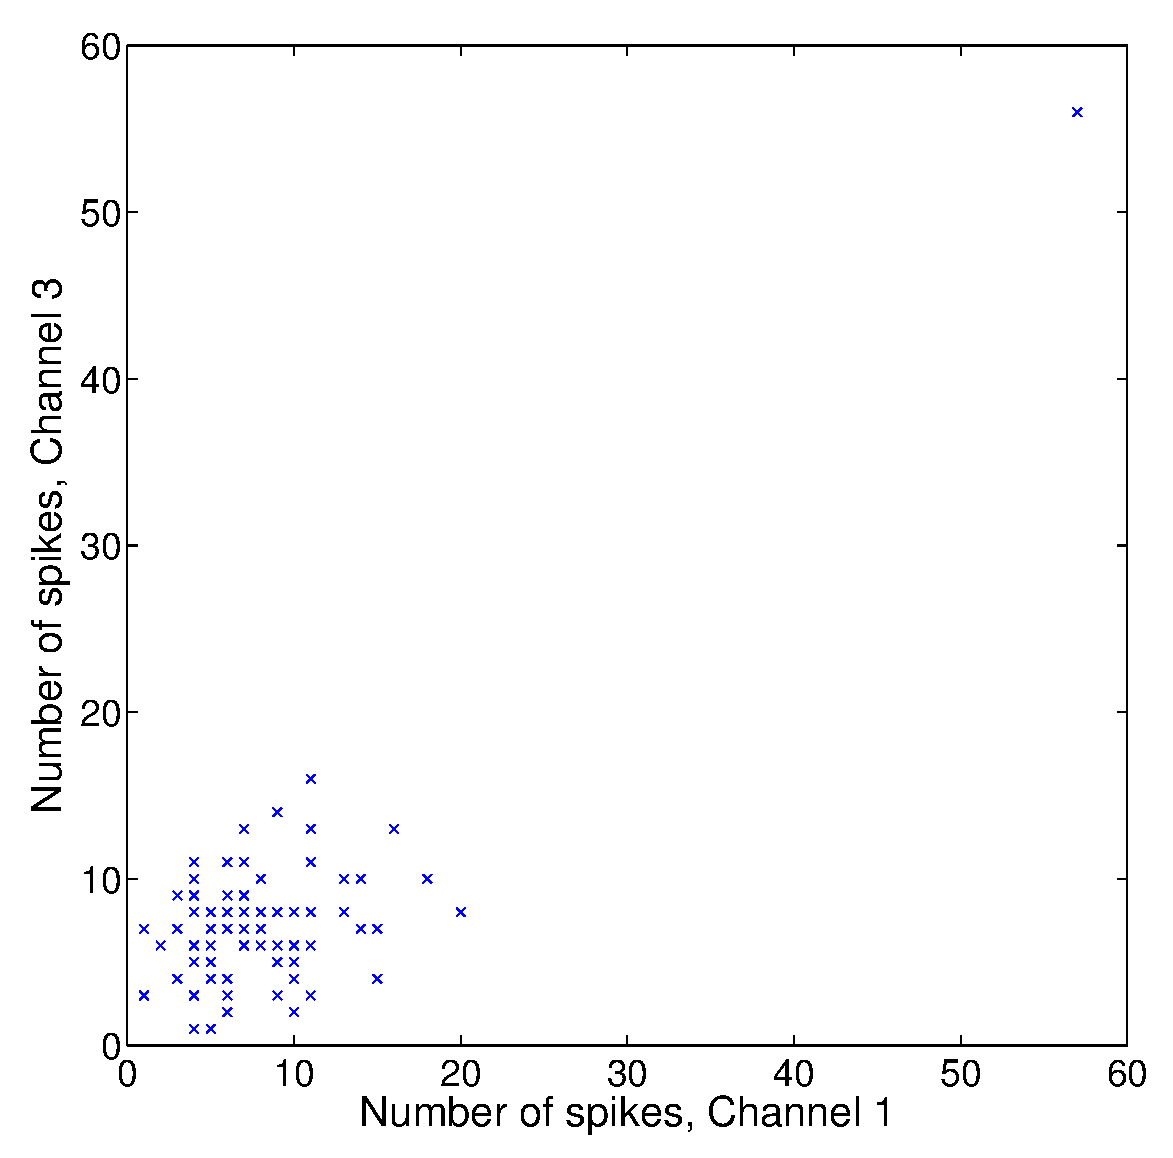
\includegraphics[width=0.4\linewidth]{%
figs/decoding/rcoef_scatter_jv4_icond5_ch1vch3.eps}
\caption{Spikes count during around \SI{500}{ms} of presentation of the \SI{27}{\percent} contrast stimulus, for two channels plotted against each other.
There is clearly a weak correlation between the two data-series, but one trial is an outlier with a large number of measured spikes for both channels due to a correlated source of noise in the raw signal.
The outlier will cause the correlation to be measured anomalously high.}
\label{fig:noise_scatter}
\end{figure}

To counter this problem, all trials where at least a quarter of the channels had a number of spikes more than 2.5 standard deviations above their mean spike count were removed.
This should be effective at fixing the problem because the motion-triggered artifact occurs always effects multiple channels simultaneously with the same artifact.


\subsection{Results}

For both \ac{V1} and \ac{V4}, the average noise correlation between pairs of channels seem to remain stable for \ac{M1} and decrease by a small margin for \ac{M2} (see Fig.~\ref{fig:noise_r_all}).
The increase in noise correlation for \ac{M1} \ac{V1} for the last two sessions (session numbers 358 and 359) is due to a decline in data quality and an increase in noise from artificial sources.
There is a large amount of variance in the noise correlations for different pairs, so the decline in mean correlation for \ac{M2} does not seem very large considering the amount of variance.


% % \begin{figure}[htb]
% %     \begin{subfigure}[b]{0.5\linewidth}
% %         \centering
% %         \caption{}
% %         \label{fig:noise_r_v1_all}
% % %         \includegraphics[width=\linewidth]{%
% % % ./rcoef_2013-04-09/rcoef_sess_meanpc_2013-04-09/png/rcoef_sess_meanpc_v1_both.png}
% % %        \includegraphics[width=\linewidth]{figs/decoding/rcoef_sess_meanpc_v1_both}
% %         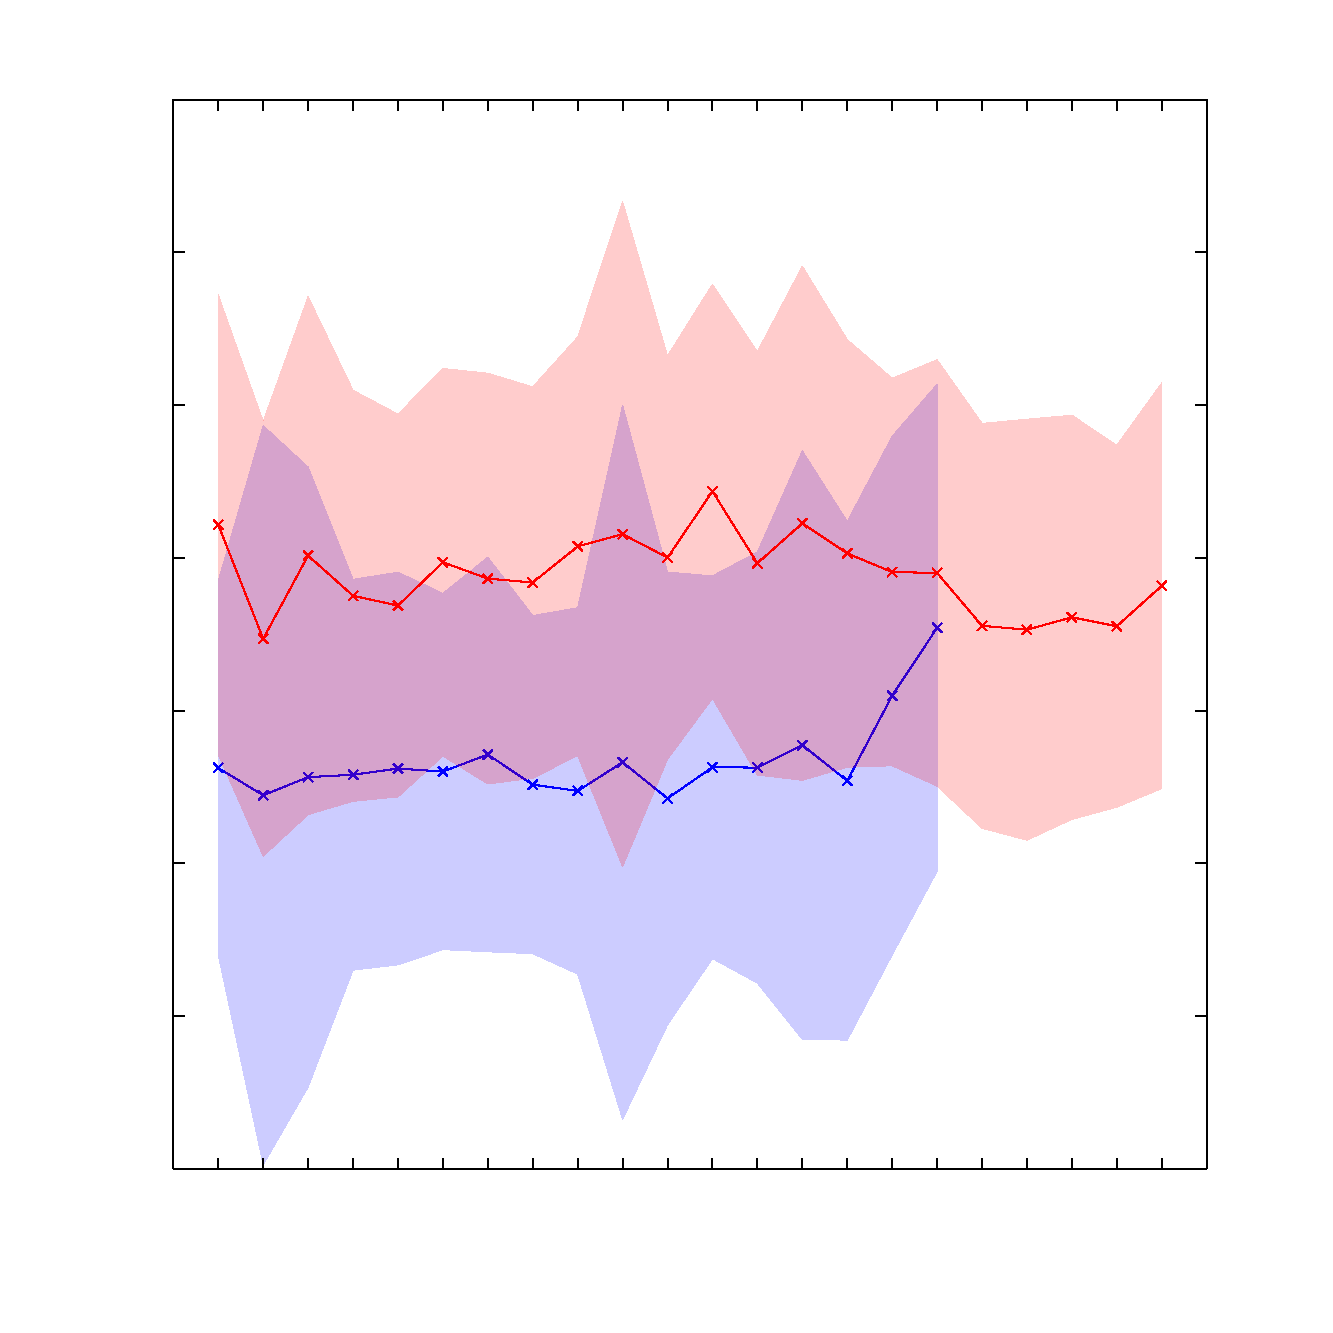
\includegraphics[width=\linewidth]{figs/decoding/rcoef_sess_meanpc_v1_both.pdf}
% %     \end{subfigure}
% %     ~~
% %     \begin{subfigure}[b]{0.5\linewidth}
% %         \centering
% %         \caption{}
% %         \label{fig:noise_r_v4_all}
% % %         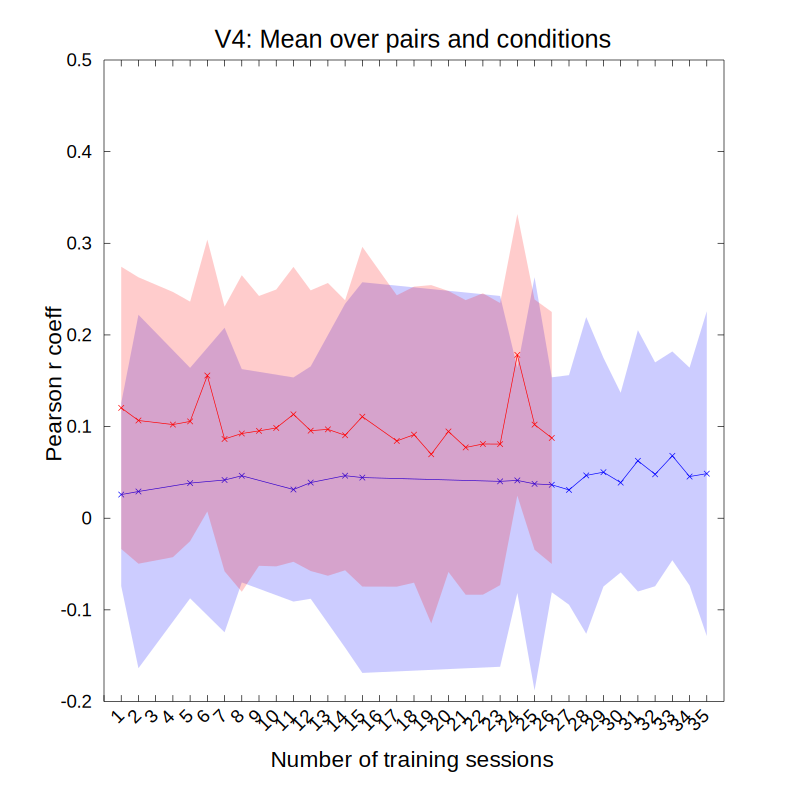
\includegraphics[width=\linewidth]{%
% % % ./rcoef_2013-04-09/rcoef_sess_meanpc_2013-04-09/png/rcoef_sess_meanpc_v4_both.png}
% %         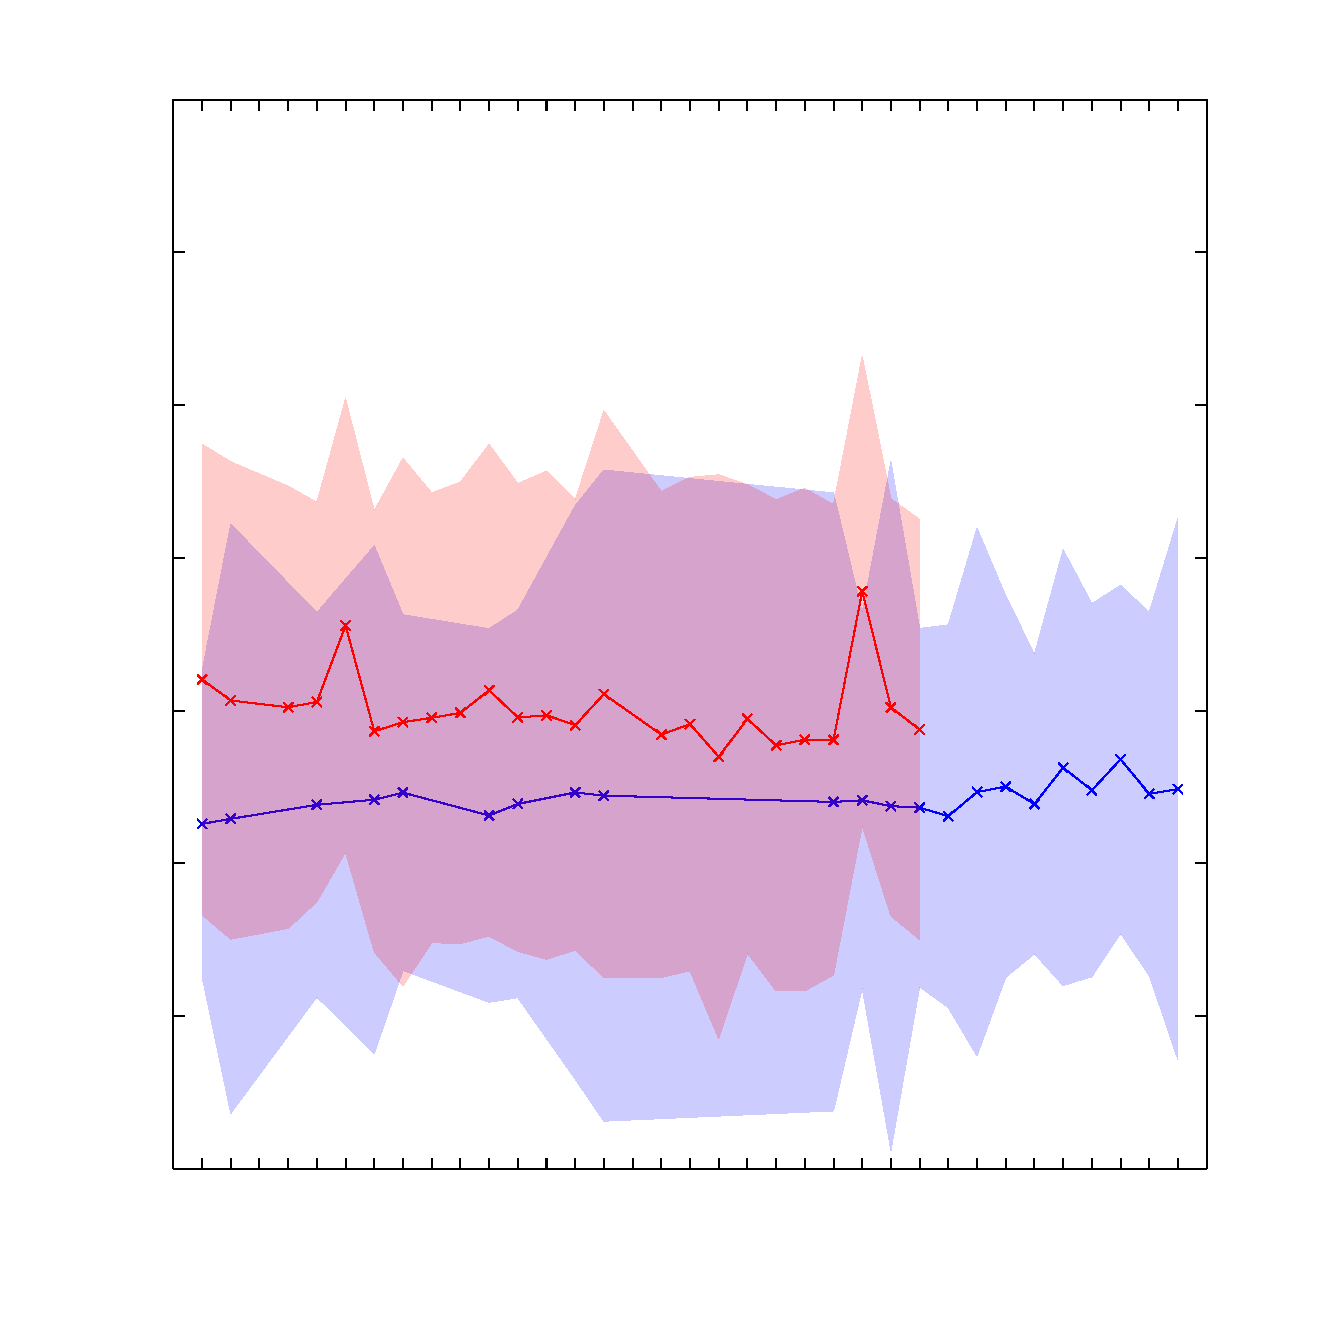
\includegraphics[width=\linewidth]{figs/decoding/rcoef_sess_meanpc_v4_both.pdf}
% %     \end{subfigure}
% %     \caption{Change in noise correlations with learning.
% % \protect\subref{fig:noise_r_v1_all}:~\ac{V1}.
% % \protect\subref{fig:noise_r_v4_all}:~\ac{V4}.
% % Blue:~\ac{M1}.
% % Red:~\ac{M2}.
% % On the x-axis, the number of sessions since the animal began training in the part of the visual field retinotopic to the recording site is shown.
% % Line: pearson r coefficient, averaged across the possible pairings between channels for each of the 14 trial conditions.
% % Shaded region indicates one standard deviation from mean.
% % }
% %     \label{fig:noise_r_all}
% % \end{figure}
% \marginnote{In Fig.~\ref{fig:noise_r_all} and \ref{fig:noise_r_hist}, the text is too small due to saving the figure with transparencies in PNG format; if I could get the SVG to load correctly, the text would be sized correctly.}

Fig.~\ref{fig:noise_r_hist} is intended to reproduce Figure 2C from \citet{Gu2011}, with the distribution of $r$ shown across pairs for one pre-training and one post-training session.
These sessions were chosen from a restricted set of sessions which did not have problems with artificially high correlations from the motion artifact, and selected from this set such that they were as close to the start and end of the training period as possible.
However, this selection was made before the set of trials was redacted as mentioned in \S\ref{sec:dec-meth-noise}, so the sessions selected could possibly be made further apart.

The data presented in Fig.~\ref{fig:noise_r_hist} shows that the distribution of noise correlation pairs does not move significantly for \ac{M1} \ac{V1}, which is contrasted by a clear decrease for \ac{M2} \ac{V1}.
It should be noted though that the distribution for \ac{M2} \ac{V1} begins higher than \ac{M1} and decreases to a similar value as \ac{M1} \ac{V1}.
For \ac{V4}, there is an increase in mean noise correlation for \ac{M1} and a decrease for \ac{M2}, though as \ac{M2} begins higher than \ac{M1} the two do tend toward to one another.

Cherry-picking is a significant problem here, as there is sizable day-to-day variation in the noise correlation across the pairs.
Choosing a session where there is more noise correlation than neighbouring sessions at the beginning of training and less at the end of training will give the impression that there is a more significant decrease in noise correlations.
More effort should be made to counter inadvertently cherry-picking in the session selection, as Fig.~\ref{fig:noise_r_j1_pmc} indicates this may be one reason for such a sizable decrease in noise correlation for \ac{M2} \ac{V1}.

\begin{figure}[htbp]
    \begin{subfigure}[b]{0.5\linewidth}
        \centering
        \caption{}
        \label{fig:noise_r_b1_hist}
%         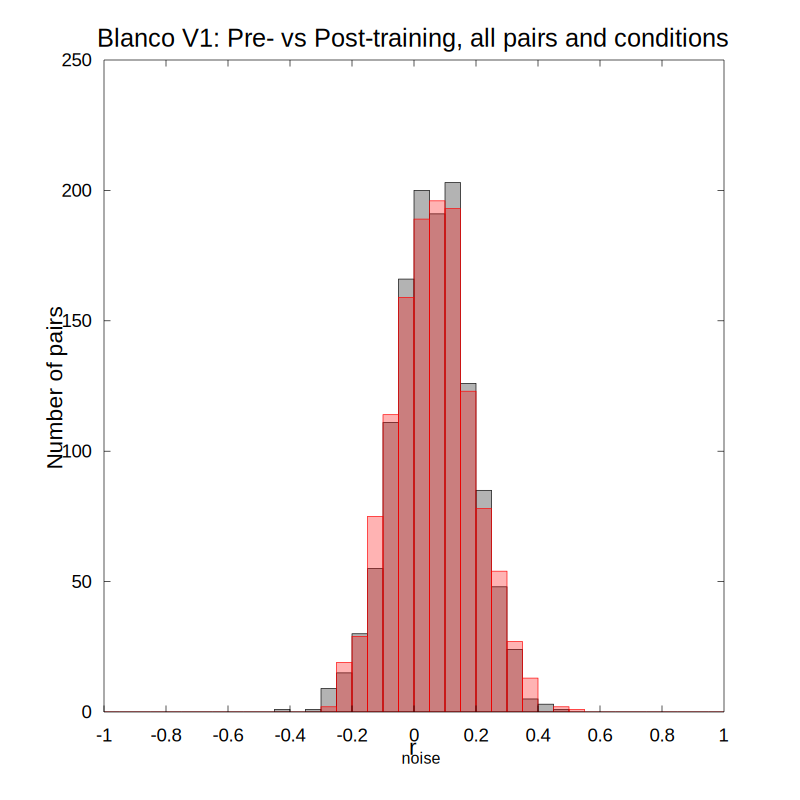
\includegraphics[width=\linewidth]{%
% ./rcoef_2013-03-25/rcoef_sess_histallover_2013-03-25/png/rcoef_sess_histallover_v1_blanco.png}
        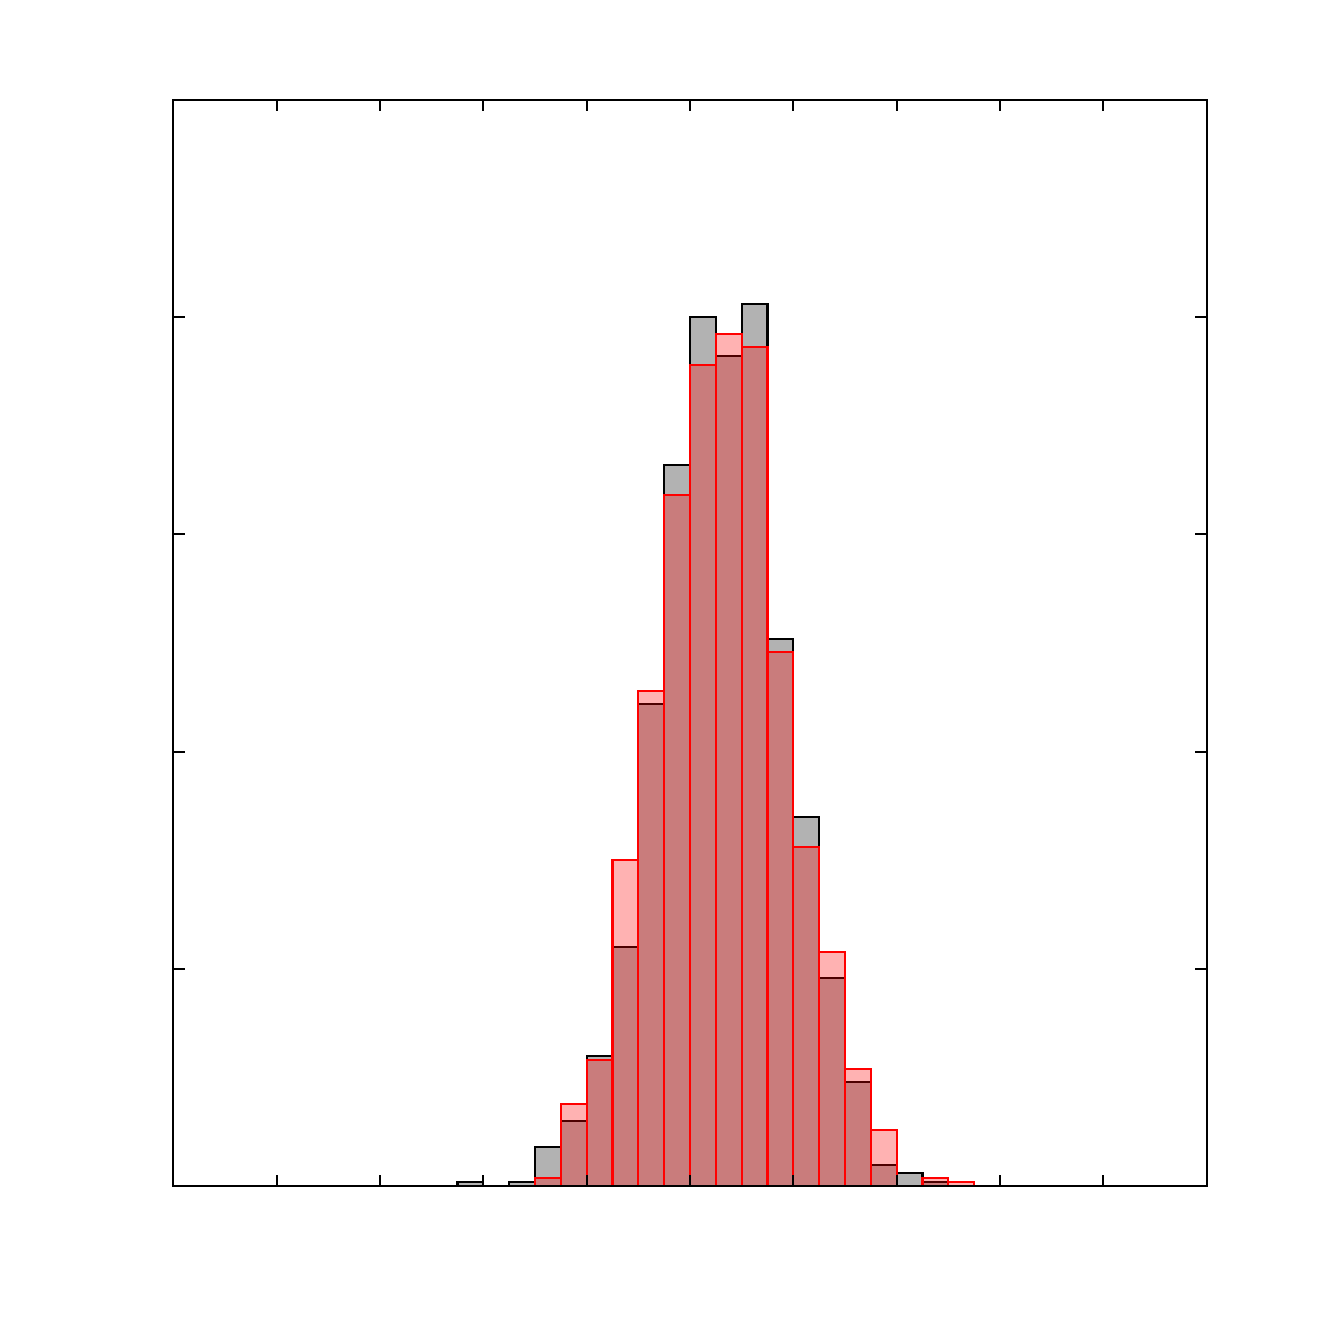
\includegraphics[width=\linewidth]{figs/decoding/rcoef_sess_histallover_v1_blanco.pdf}
    \end{subfigure}
    ~~
    \begin{subfigure}[b]{0.5\linewidth}
        \centering
        \caption{}
        \label{fig:noise_r_j1_hist}
%         \includegraphics[width=\linewidth]{%
% ./rcoef_2013-03-25/rcoef_sess_histallover_2013-03-25/png/rcoef_sess_histallover_v1_jack.png}
        \includegraphics[width=\linewidth]{figs/decoding/rcoef_sess_histallover_v1_jack.pdf}
    \end{subfigure}
    \\
    \begin{subfigure}[b]{0.5\linewidth}
        \centering
        \caption{}
        \label{fig:noise_r_b4_hist}
%         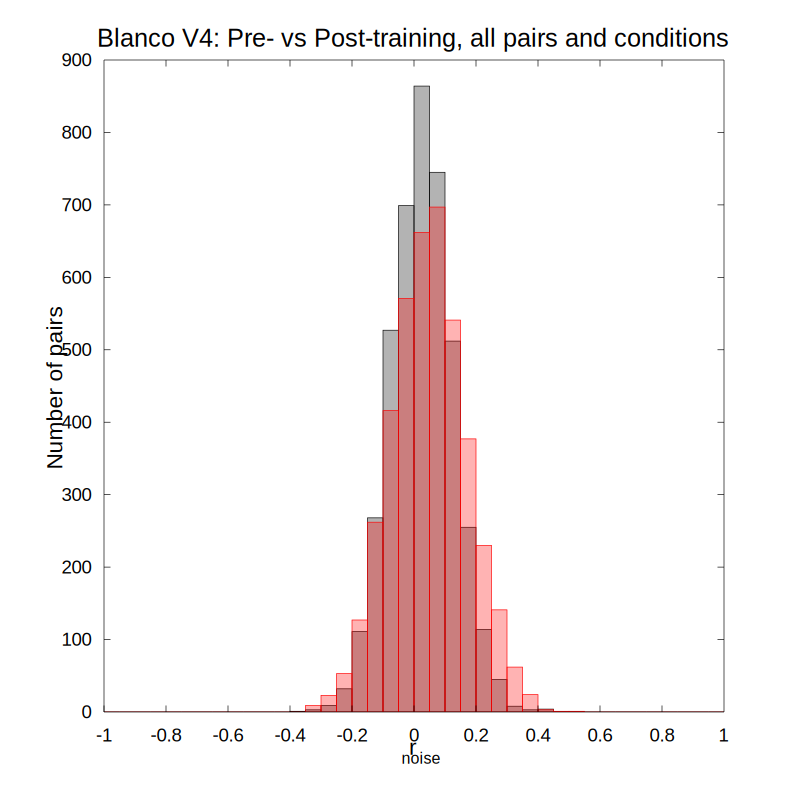
\includegraphics[width=\linewidth]{%
% ./rcoef_2013-03-25/rcoef_sess_histallover_2013-03-25/png/rcoef_sess_histallover_v4_blanco.png}
        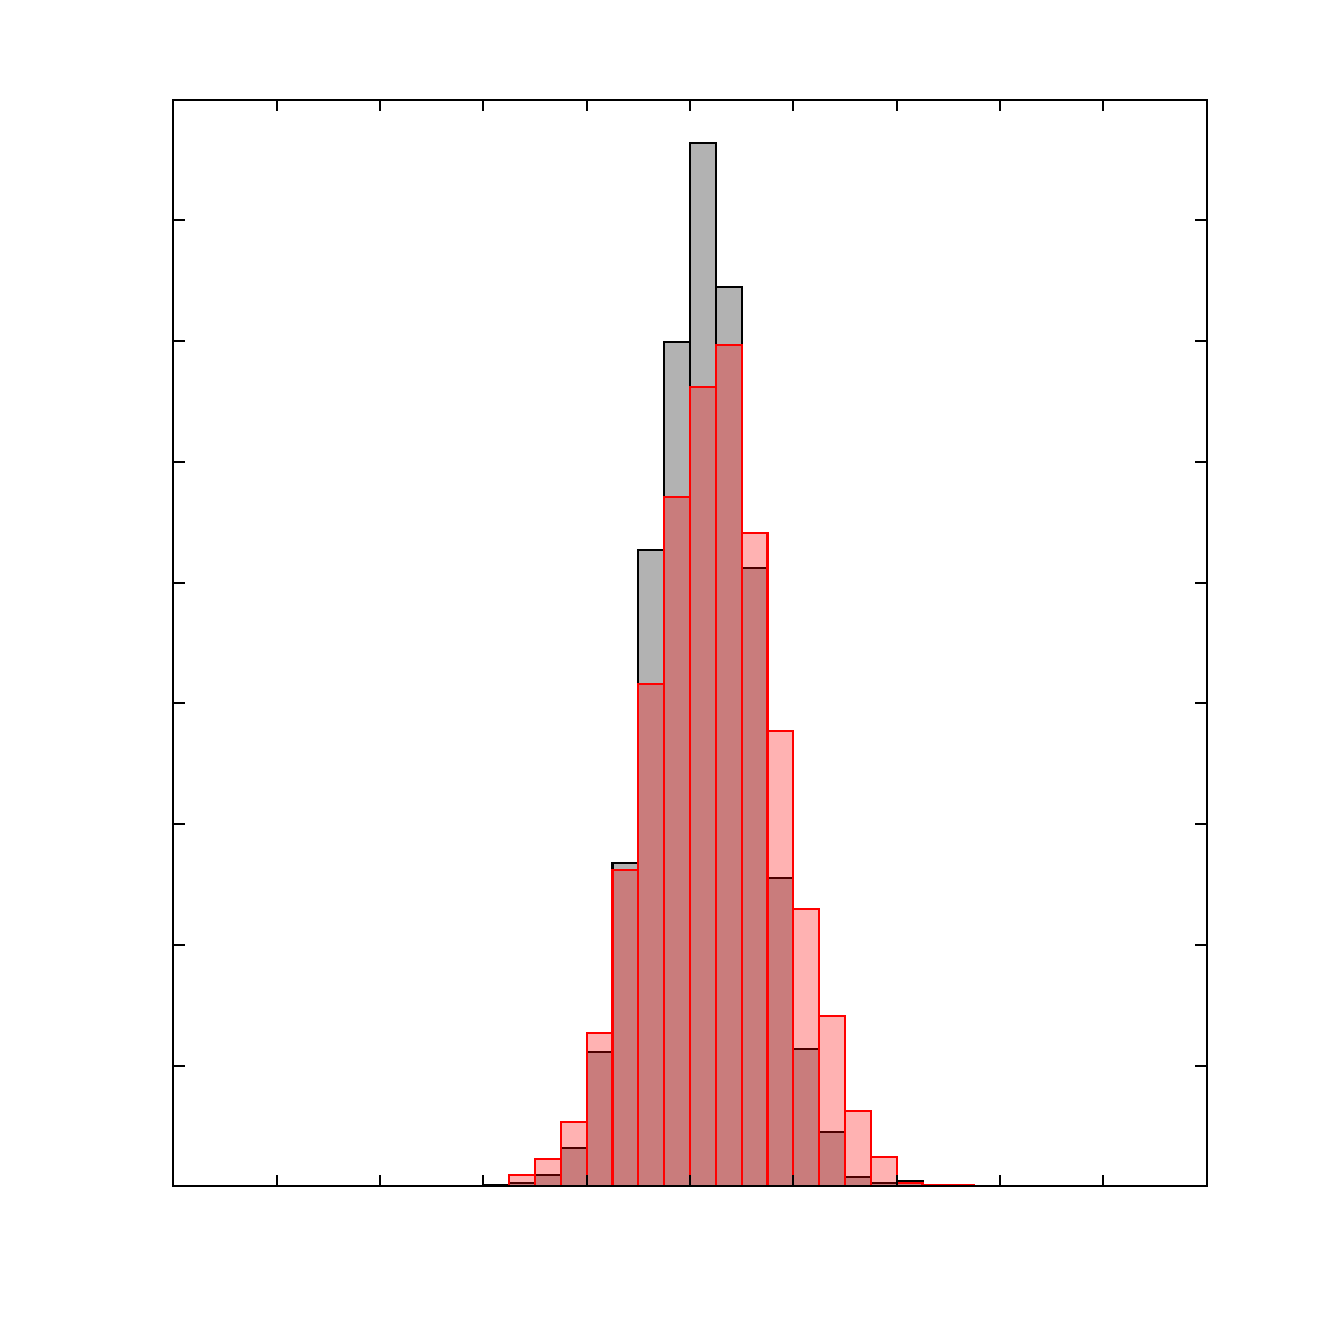
\includegraphics[width=\linewidth]{figs/decoding/rcoef_sess_histallover_v4_blanco.pdf}
    \end{subfigure}
    ~~
    \begin{subfigure}[b]{0.5\linewidth}
        \centering
        \caption{}
        \label{fig:noise_r_j4_hist}
%         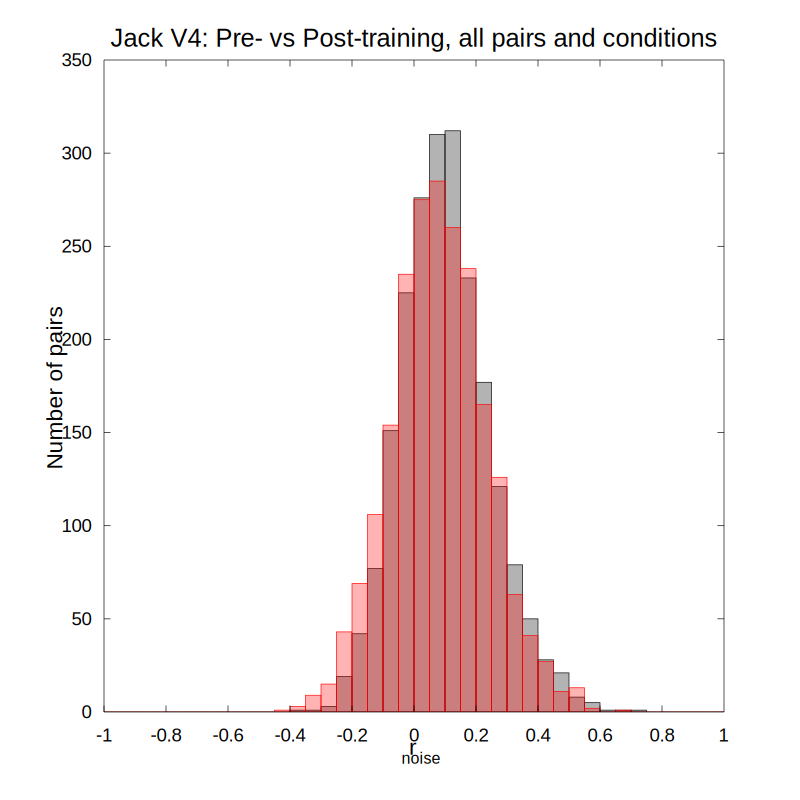
\includegraphics[width=\linewidth]{%
% ./rcoef_2013-03-25/rcoef_sess_histallover_2013-03-25/png/rcoef_sess_histallover_v4_jack.png}
        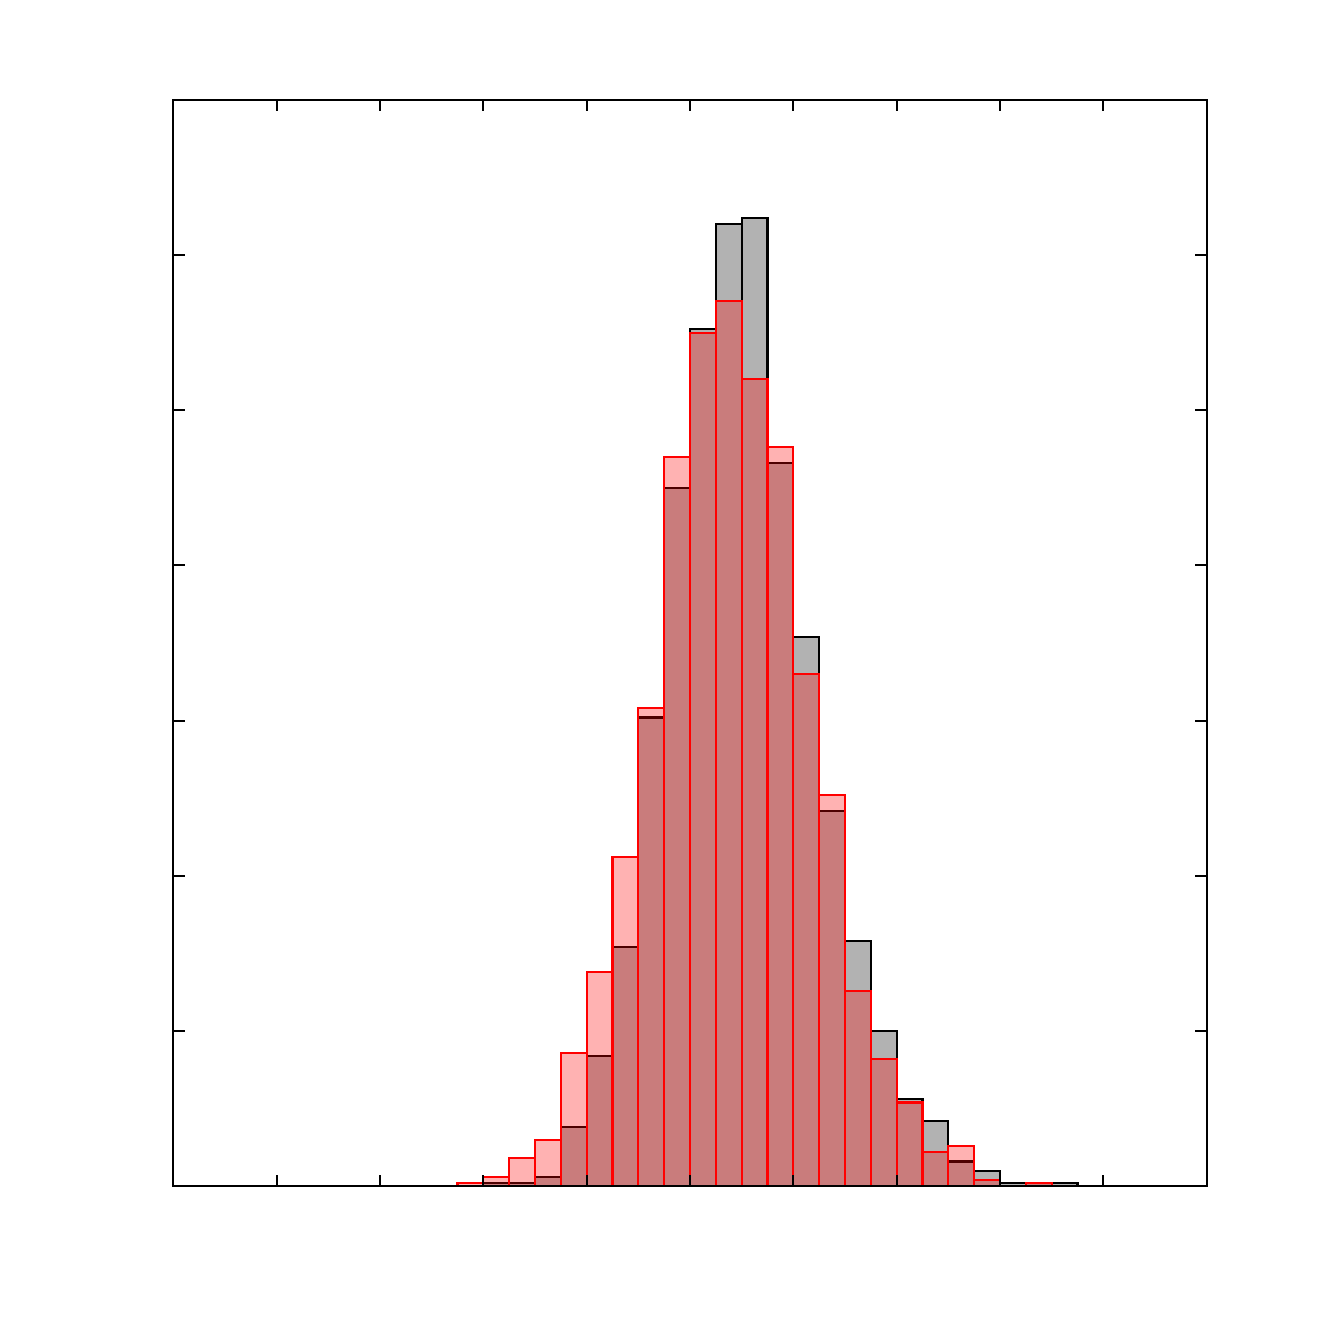
\includegraphics[width=\linewidth]{figs/decoding/rcoef_sess_histallover_v4_jack.pdf}
    \end{subfigure}
    \caption{Distribution of the noise correlations for the pairings across all conditions.
Two sessions, one at the beginning of training (black) and one at the end of training (red) are shown for comparitive purposes.
\protect\subref{fig:noise_r_b1_hist}: \ac{M1} \ac{V1}; sessions 343 and 354.
\protect\subref{fig:noise_r_j1_hist}: \ac{M2} \ac{V1}; sessions 51 and 71.
\protect\subref{fig:noise_r_b4_hist}: \ac{M1} \ac{V4}; sessions 307 and 338.
\protect\subref{fig:noise_r_j4_hist}: \ac{M2} \ac{V4}; sessions 27 and 46.
}
    \label{fig:noise_r_hist}
\end{figure}


% Fig.~\ref{fig:noise_r_pmc} indicates that noise correlations are correlated for pairs across sessions.
A pairs of channels which have higher noise correlations in one session are likely to have higher noise correlation in other sessions.
However, this effect is not present for \ac{M1} \ac{V1}, Fig.~\ref{fig:noise_r_b1_pmc}, and could suggest there is less session-to-session consistency for this dataset.

This figure provides an easy way of visually inspecting whether noise correlations are conserved, but does not allow us to quantify this.

\begin{figure}[htbp]
    \begin{subfigure}[b]{0.5\linewidth}
        \centering
        \caption{}
        \label{fig:noise_r_b1_pmc}
        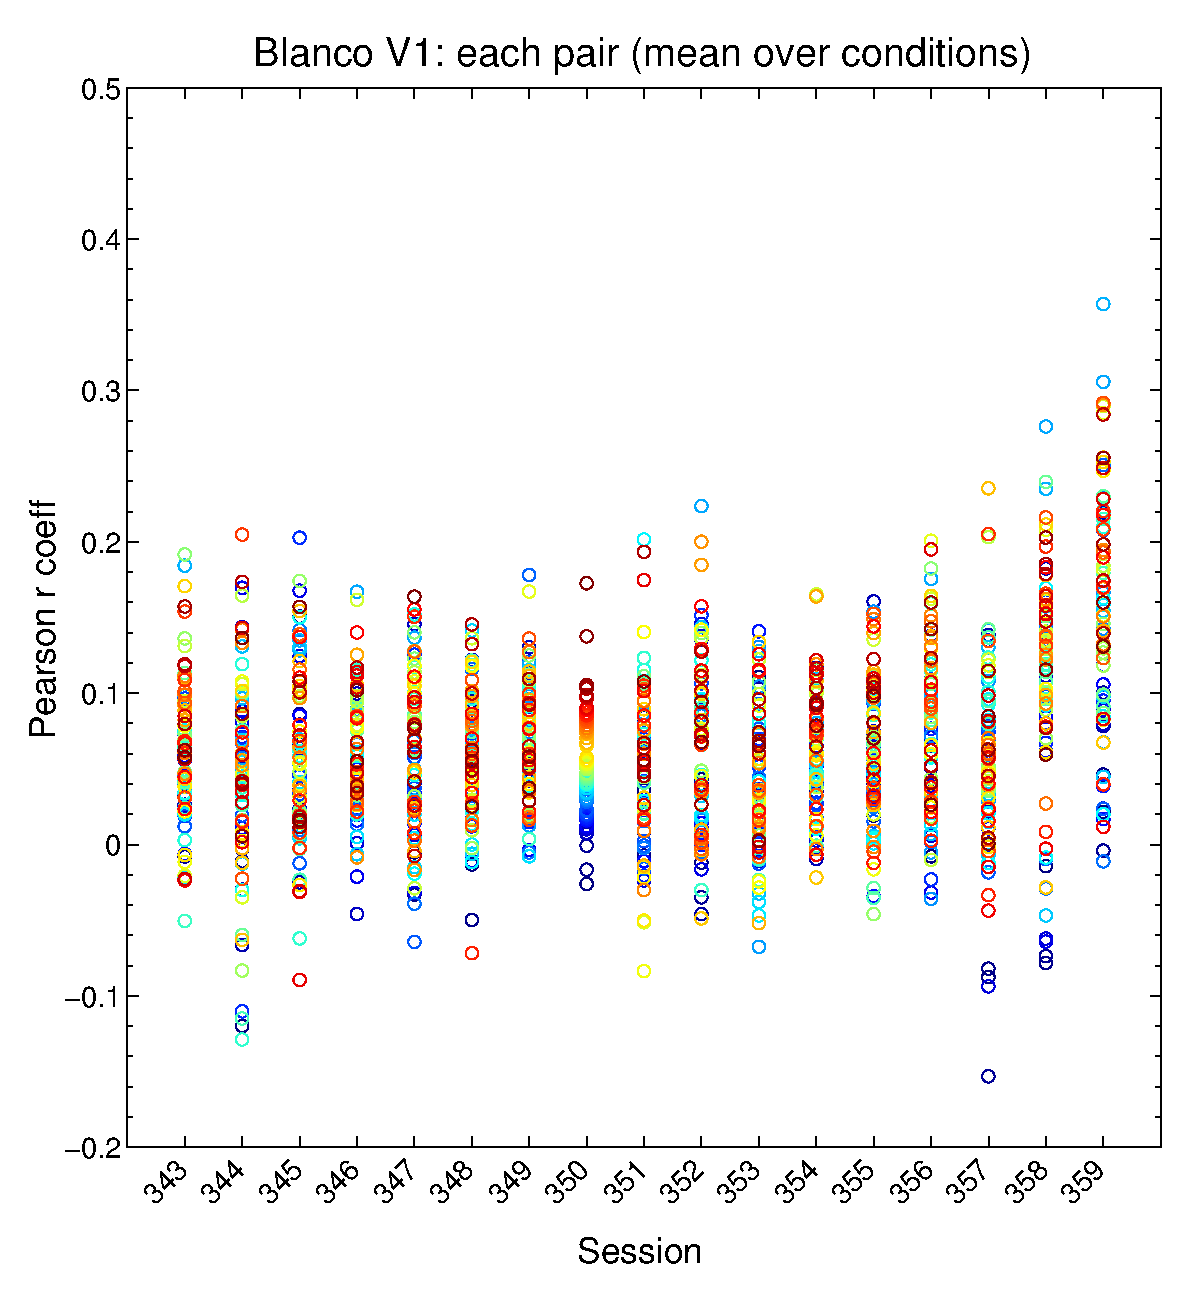
\includegraphics[width=\linewidth]{%
figs/decoding/rcoef_sess_pairsmeanc_v1_blanco.eps}
    \end{subfigure}
    ~~
    \begin{subfigure}[b]{0.5\linewidth}
        \centering
        \caption{}
        \label{fig:noise_r_j1_pmc}
        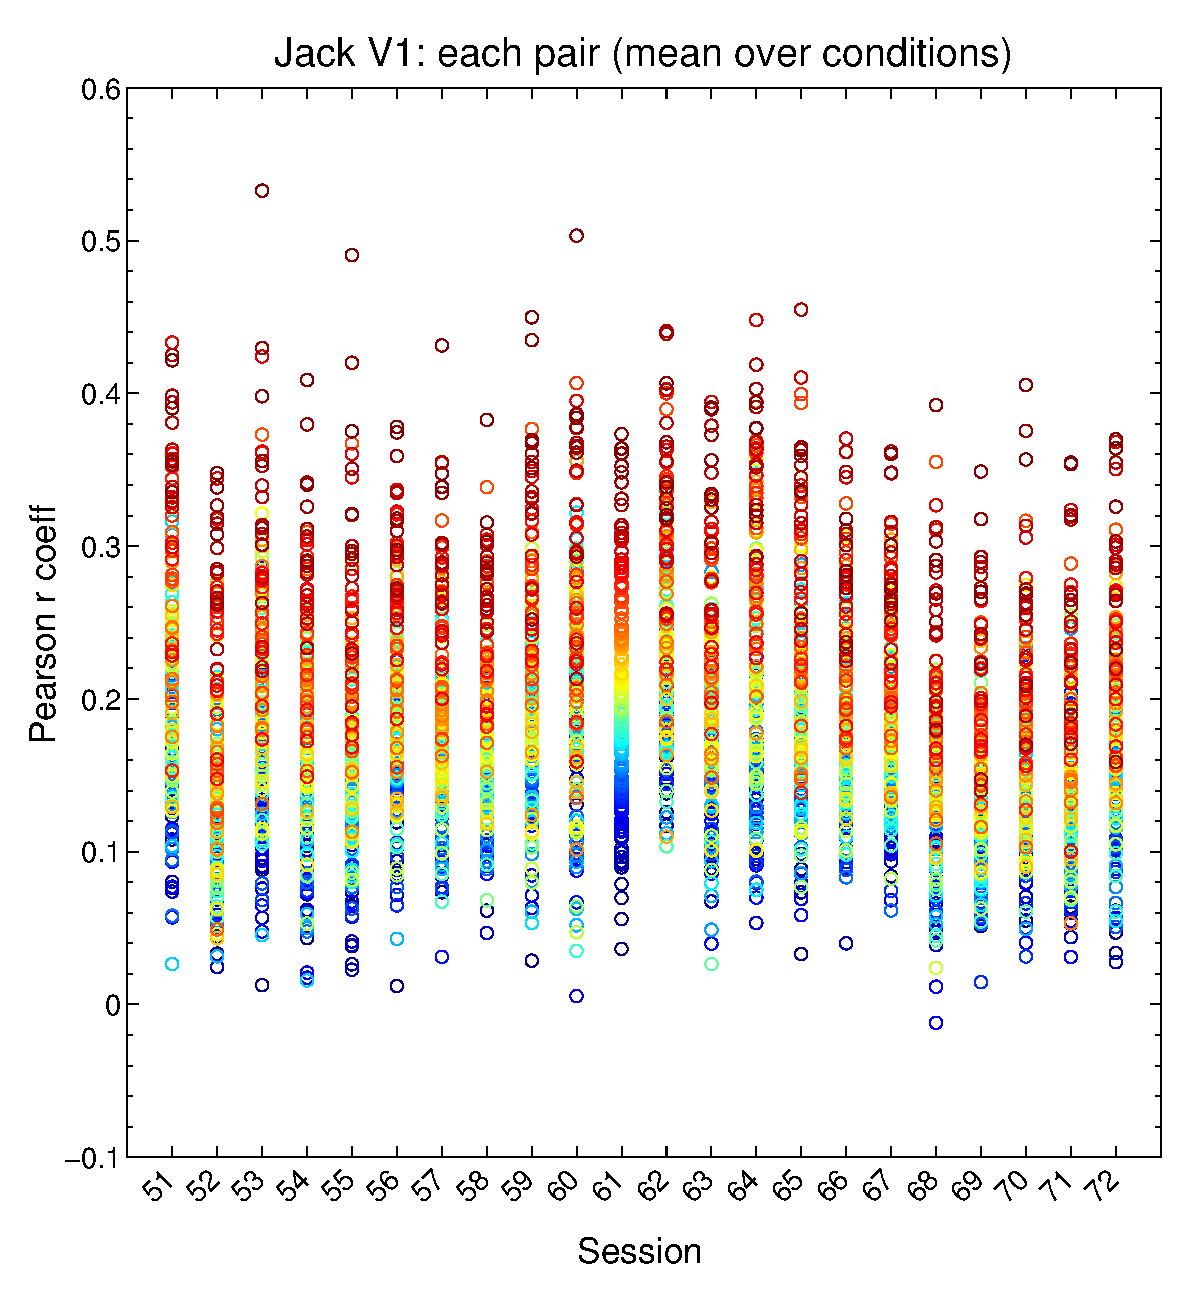
\includegraphics[width=\linewidth]{%
figs/decoding/rcoef_sess_pairsmeanc_v1_jack.eps}
    \end{subfigure}
    \\
    \begin{subfigure}[b]{0.5\linewidth}
        \centering
        \caption{}
        \label{fig:noise_r_b4_pmc}
        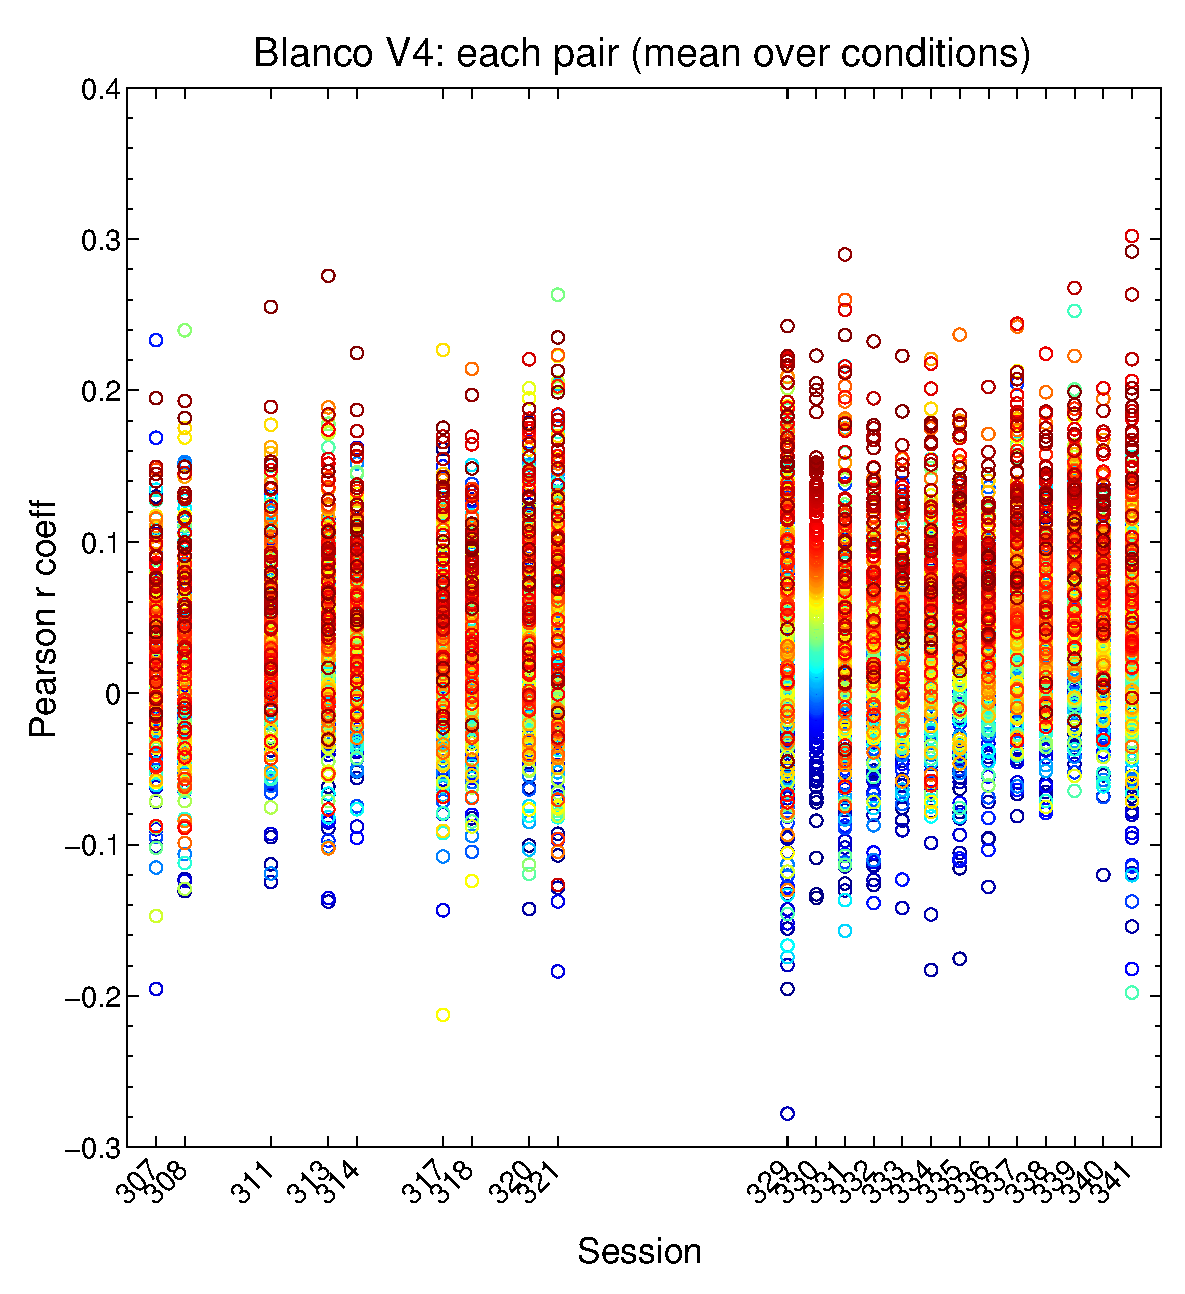
\includegraphics[width=\linewidth]{%
figs/decoding/rcoef_sess_pairsmeanc_v4_blanco.eps}
    \end{subfigure}
    ~~
    \begin{subfigure}[b]{0.5\linewidth}
        \centering
        \caption{}
        \label{fig:noise_r_j4_pmc}
        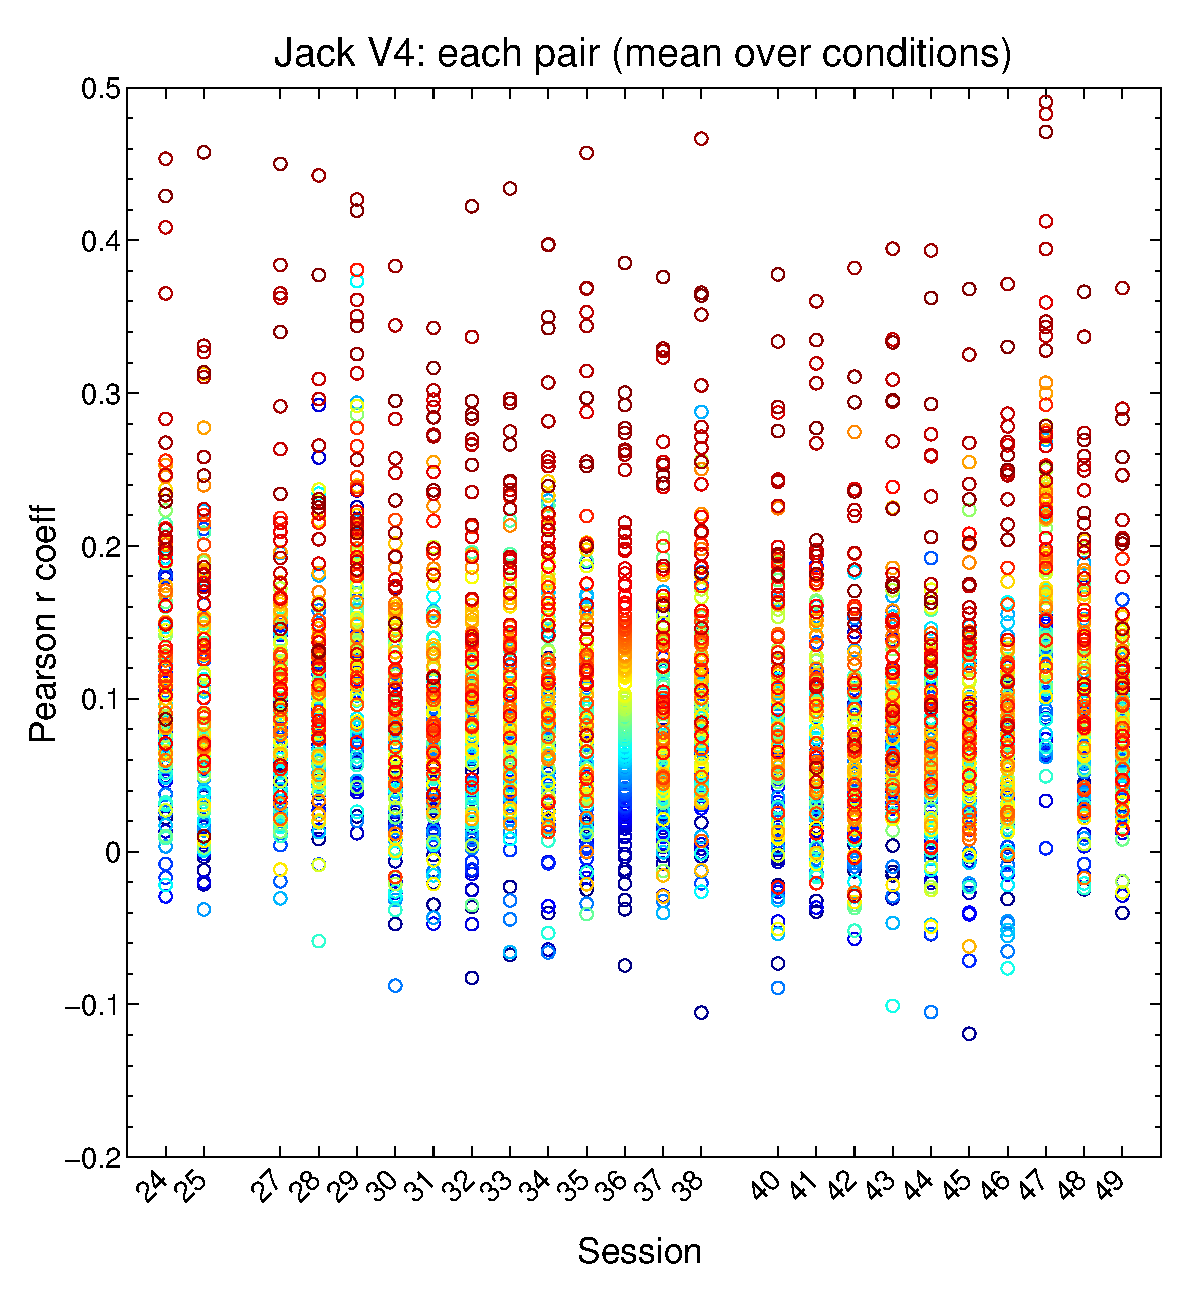
\includegraphics[width=\linewidth]{%
figs/decoding/rcoef_sess_pairsmeanc_v4_jack.eps}
    \end{subfigure}
    \caption{Noise correlations for each pair, meaned across the 14 conditions.
\protect\subref{fig:noise_r_b1_pmc}: \ac{M1} \ac{V1}.
\protect\subref{fig:noise_r_j1_pmc}: \ac{M2} \ac{V1}.
\protect\subref{fig:noise_r_b4_pmc}: \ac{M1} \ac{V4}.
\protect\subref{fig:noise_r_j4_pmc}: \ac{M2} \ac{V4}.
Colour is assigned by sorting the pairs into ascending order for one of the sessions near the middle of the training period.
The degree of session-to-session correlation of the noise correlation can hence be inferred by visual inspection.
}
    \label{fig:noise_r_pmc}
\end{figure}


% %==============================================================================
% \section{$d'$ Analysis}
% %------------------------------------------------------------------------------
%
% In an attempt to clean up the data and only use the channels and sessions which provide the most relevant results
%
% Discriminating based on the information content in the channels would allow us to ``cherry-pick'' the best data and artificially inflate the results, so an independent metric of data quality was sought.
% Since we are interested in the channels where the data is of reasonable quality and the neurons represented by the channel are responsive to the stimulus, $d'$ was used.
%
% $d'$ is ...
%
% %------------------------------------------------------------------------------
% \subsection{Methods}
%
% % How is it computed?
%
% % $$
% % \mu_{stim} = mean(a_{stim});
% % \mu_{spon} = mean(a_{spon});
% % 
% % % Combine the standard deviations of the two sets of trials
% % % Have to do a weighted average of the variances
% % stdev_joint = sqrt(...
% %     ( (n_stim-1)*var(act_stim) + (n_spon-1)*var(act_spon) ) ...
% %     / (n_stim + n_spon - 2) ...
% %     );
%
% $$
% d\,' = \frac{\mu_{stim} - \mu_{spon}}{\sigma_{joint}}
% ,$$
% where the joint standard deviation over both populations is given by 
% $$
% \sigma_{joint} = \sqrt
%     \frac{ (n_{stim}-1) \, \sigma_{stim} + (n_{spon}-1) \, \sigma_{spon} }
%     { n_{stim} + n_{spon} - 2}
% $$
% so that it is weighted by the number of datapoints, $n_{stim}$ and $n_{spon}$, for both the stimulus presentation and spontaneous activity 
%
% References
% Compared the mean firing rate for spontaneous activity and the sample stimulus of 30\% contrast
% Compared the mean firing rate for spontaneous activity and the highest contrast test stimulus
%
% %------------------------------------------------------------------------------
% \subsection{Results}
%
% d' increases with learning
%
% Just using channels with a session-wise mean d' > X gives us cleaner results


%==============================================================================
\section{Decoder-based methods}
\label{sec:dec-meth-lin}
%------------------------------------------------------------------------------

The input data to the decoding algorithm was chosen to be the total spike count during stimulus presentation from each trial.
This total is taken only for channels known to offer a consistent firing rate across sessions after the spontaneous activity matching process.
If there are 20 such channels in the dataset, taking the total number of spikes during stimulus presentation for each of the channels results in a 20-dimensional vector of population activity on each trial.

It should be noted that using all the spikes during the stimulus presentation period is likely to be sub-optimal, as not necessarily all of this period of time is carrying useful information about the stimuli.
The amount of spikes before the onset response, for instance, is clearly not stimulus dependent as it precedes the neural response to the stimulus, so it will only be a source of noise and  not useful for the decoding.
Furthermore, it is possible that the firing rate during the onset response might be more informative than the average firing rate across the whole presentation period.
However, finding the optimal window from which to take the spikes is an exercise in of itself.

The decoder used was a Fisher linear discriminant classifier.
Given a training dataset of labelled data points in 20D, the classifier will find the optimal 19D hyperplane such that it separates the two classes of points optimally, under the assumption that the two clusters to be separated are multivariate normal distributions.
The vector normal to the hyperplane is 
\begin{equation}
\vec{w} = \Sigma^{-1}\left(\vec{\mu_1}-\vec{\mu_0}\right)
\end{equation}
where $\Sigma$ is the covariance matrix between the two populations, as determined from the available labelled data, and $\vec{\mu_0}$ and $\vec{\mu_1}$ are the computed means of the two distributions.

Once a classifying hyperplane has been found, test data points can be classified by observing the side of the hyperplane on which they fall.
For a new data point, $\vec{x}$,  if
\begin{equation}
\vec{w}\cdot\vec{x}>c
\end{equation}
then we classify $\vec{x}$ as group 1 (higher than \SI{30}{\percent} contrast), otherwise we classify it as 0 (lower).

This was performed using the function \texttt{classify} with type `linear' in MATLAB.
For training and testing of the decoder, leave-one-out classification was used across each session individually.
This means that for a session of 500 trials, the decoder is trained on 499 trials with the spike counts for all the trials and the correct response (higher or lower than \SI{30}{\percent} contrast) and we then check whether the decoder identifies the remaining trial correctly.
This is repeated for all the 500 trials, and then the performance is defined as the proportion of trials which are identified correctly.
Training the decoder in this way means the decoding hyperplane used for classification is optimal for each individual session, but also different for each session.

The impact of noise correlations on the decoder is considered by comparing the regular decoder performance with the performance of a decoder applied to data which has been shuffled across trials under the same stimulus conditions.
After shuffling, specific neural response vectors no longer correspond to any particular trial, since the spike counts for each channel are taken from different trials.

%------------------------------------------------------------------------------
\subsection{Probabilistic Model}
\label{sec:dec-meth-prob}

As well as comparing the behavioural and decoding responses with the target responses to find a value for predictor performance, we can compare the behavioural and decoding responses with one another and find a value for their agreement, the proportion of trials on which the two responses are the same.

We would like to evaluate whether the behavioural responses are dependent on the firing rates of the recorded population of neurons.
This can be done by considering the behavioural and decoding response agreement, but in order to do this we need to construct a model of how much agreement we would expect to find if the two were completely independent, which will form our null hypothesis (NH) to compare against.

Throughout this work, it is assumed that the behavioural and decoding responses are given by a Bernoulli distribution.
In this model, there is a true probability, $p$, of the animal giving the correct answer to the task for each trial, which is sampled from on each of the trials.
When this is sampled over $n$ trials, we expect to find $np$ trials have been responded correctly and $n(1-p)$ incorrectly.

Hence the underlying true probability of a correct response can be approximated by taking the number of correct responses and dividing them by the total number of trials.
Using one of several statistical methods, we can find an estimate for a percentage confidence interval (PCI).
It is from this that error bars, indicated by the shaded regions surrounding line plots in Figs.~\ref{fig:dec_all_v1} and ~\ref{fig:dec_all_v4}, are computed.
These are presented as the standard error, equivalent to a \SI{31.8}{\percent}  confidence interval within which \SI{68.2}{\percent} of data points are expected to lie.
(This has been done using the function \texttt{binofit} in MATLAB, which utilises the Clopper-Pearson method.
Although this is not the best method, it should be sufficient for our purposes.)

The behavioural performance is given by the estimated probability of the behavioural response being the same as the correct response, simply found by dividing the number of times the behavioural response matched the target response by the number of presentations.
The target response is of course whether or not the test stimulus is actually higher or lower than the sample.
Similarly, the decoding performance is the proportion of times the decoding response is the same as the target response; and the behavioural and decoding agreement is the proportion of times the behavioural and decoding responses are the same.

Using the estimated probabilities of the behavioural and decoding responses being correct, we can find an expected agreement between the behavioural and decoding responses if they are completely independent of one another, which constitutes the null hypothesis model (NH).
By comparing the observed agreement with the agreement we expect for independent variables, we can see whether or not behavioural responses are correlated with the decoded neural responses.

The theory behind the estimation of the agreement for independent binomial processes is described as follows.
Let us take two independent binomial variables, $X_1$ and $X_2$, which can either be in state $s_1$ with probabilities $p_1$ and $p_2$ respectively, or in state $s_2$ with probability $(1-p_1)$ and $(1-p_2)$.
If $X_1$ and $X_2$ are completely independent, we expect to find them in the same state with probability $p_1 \, p_2 + (1-p_1) (1-p_2)$.
Obviously, if $p_1$ and $p_2$ are both 0.5, there is a 0.5 chance of them being in the same state.
If $p_1$ and $p_2$ are both either higher or lower than 0.5, there is a higher chance of $X_1$ and $X_2$ being in the same state, and conversely if one is above and one below 0.5, there is a lower chance of them being in the same state.
This means that if the probabilities of the behavioural and decoding responses being correct rises during the perceptual learning process, we expect the proportion of trials on which they agree to rise as well, even if the two distributions are completely independent.

The initial model for the expected agreement between behaviour and decoding used a simple model as described above, where $p_1$ and $p_2$ are taken to be the overall probability of a correct response across all the test stimuli for behaviour and decoding respectively.
We will refer to this model as the single binomial model, as each predictor is modelled with a single binomial.
However, since there are 14 possible stimuli with varying difficulty, a more detailed model can be conceived in which the probability of a correct response for each predictor depends on the stimulus presented.
In this ``multi-binomial'' model, the set of conditions (different stimuli) is given by $C$, and each predictor, $i\in\{b,d\}$, can either be in the ``lower'' or ``higher'' state ($s_l$ or $s_h$).
For each $c\in C$, there is some probability $p_{il|c} := P(x_i=s_l|c)$ of predictor a being in the lower state.
Consequently, the probability of the two predictors being in the same state is given by
$$p_a = \sum_{c\in C} P(c) (p_{bl|c} \, p_{dl|c} + (1-p_{bl|c}) (1-p_{dl|c}),$$
where $P(c)$ is the probability of condition $c$ being presented to the animal on any given trial.

We will assume that $c$ is a random variable, which is sampled from for each trial independent from prior trials.
This is a simplification of the actual condition selection process, ``delayed repetition''.
In this, the conditions for a set of trials are chosen in advance with $n$ appearances of each condition in a random order, after which any trial on which the animal responded incorrectly is repeated.
This means the single random variable approximation $P(c)$ is not uniform across the conditions, as harder conditions are presented more frequently.

For a given group of trials (such as, for instance, a single session), $P(c)$ can be estimated by dividing the number of times each appears by the total number of trials in the group.
Similarly, $p_{il|c}$ can be estimated by dividing the number of trials on which the predictor was in the lower state for a given condition by the number of trials where that condition was presented.

It is not immediately clear whether the single- or multi-binomial models will yield similar or different results.
Obviously, the multi-binomial model has more accurate detail and so should give a better result, but whether or not the single binomial should give a reasonable approximation is not obvious, though one would assume it would.
Applying the two models to the data and comparing them, we found the single binomial significantly underestimates the agreement which would really be found if the two predictors were completely independent.
Henceforth, only the more accurate multi-binomial model is considered.

The expected agreement under the assumption of two independent binomial processes gives us the null hypothesis model to compare against.
If the results of the analysis deviate significantly from this model, we can conclude the behavioural and neural decoded responses are correlated.
A $p<0.05$ significance boundary was found by sampling the NH model 100,000 times and noting the agreement for the fifth-percentile of samples.
During this sampling, the number of trials for each test condition was fixed with the same values as used in the experiment.
Since we are only interested in sessions where the behavioural and decoded responses agree more than they would if independent, a single-tailed test was used.
(NB: in the figures below, the single-tailed lower bound is also included for symmetry, so only \SI{90}{\percent} of the samples lie within the shaded region).

The multi-binomial model should not be confused with a multinomial distribution, which would map one random variable to $n$ possible responses.
The model used here is instead a two-step process where there are a set of binomial distributions, which binomial is used is determined by one random variable (the output of which is the same for both behaviour and decoder), and the output of the selected binomial is given by a second random variable.
In essence, the simple, single binomial model is similar to shuffling the responses across all trials regardless of condition, and the multi-binomial model we use is similar to shuffling the responses with the same condition presented.

%------------------------------------------------------------------------------
\subsection{Results}

Fig.~\ref{fig:dec_singles} shows how well the decoder does based only on data from individual channels.
The performance was measured as described in \S\ref{sec:dec-meth-lin} for each session, and then averaged over all sessions.
[perhaps a histogram would show how these are distributed better?]

Fig.~\ref{fig:dec_nbest} indicates how the performance of the decoder improves as more channels are added.
We can see that the decoder performance saturates after around 10 channels are included in the training data, but at a perforance which is still far from the ideal.
After this, including additional channels yields only a slight increase in performance, suggesting nearly all the information contained in the remaining channels is redundant, as it has already been given in the first 10 channels.
[would be better to look at how the decoding perfarmance is distributed across all possible sets of $n$ channels, rather than just the best set of $n$ channels] [this should be compared with shuffled data to see what the impact is and whether performance does not saturate when correlations are removed as per some previous papers [cite]]

NB: the order in which channels were added in Fig.~\ref{fig:dec_nbest} is not the same ordering as they are shown in Fig.~\ref{fig:dec_singles}.

\begin{figure}[htbp]
    \begin{subfigure}[b]{0.5\linewidth}
        \centering
        \caption{}
        \label{fig:dec_singles}
        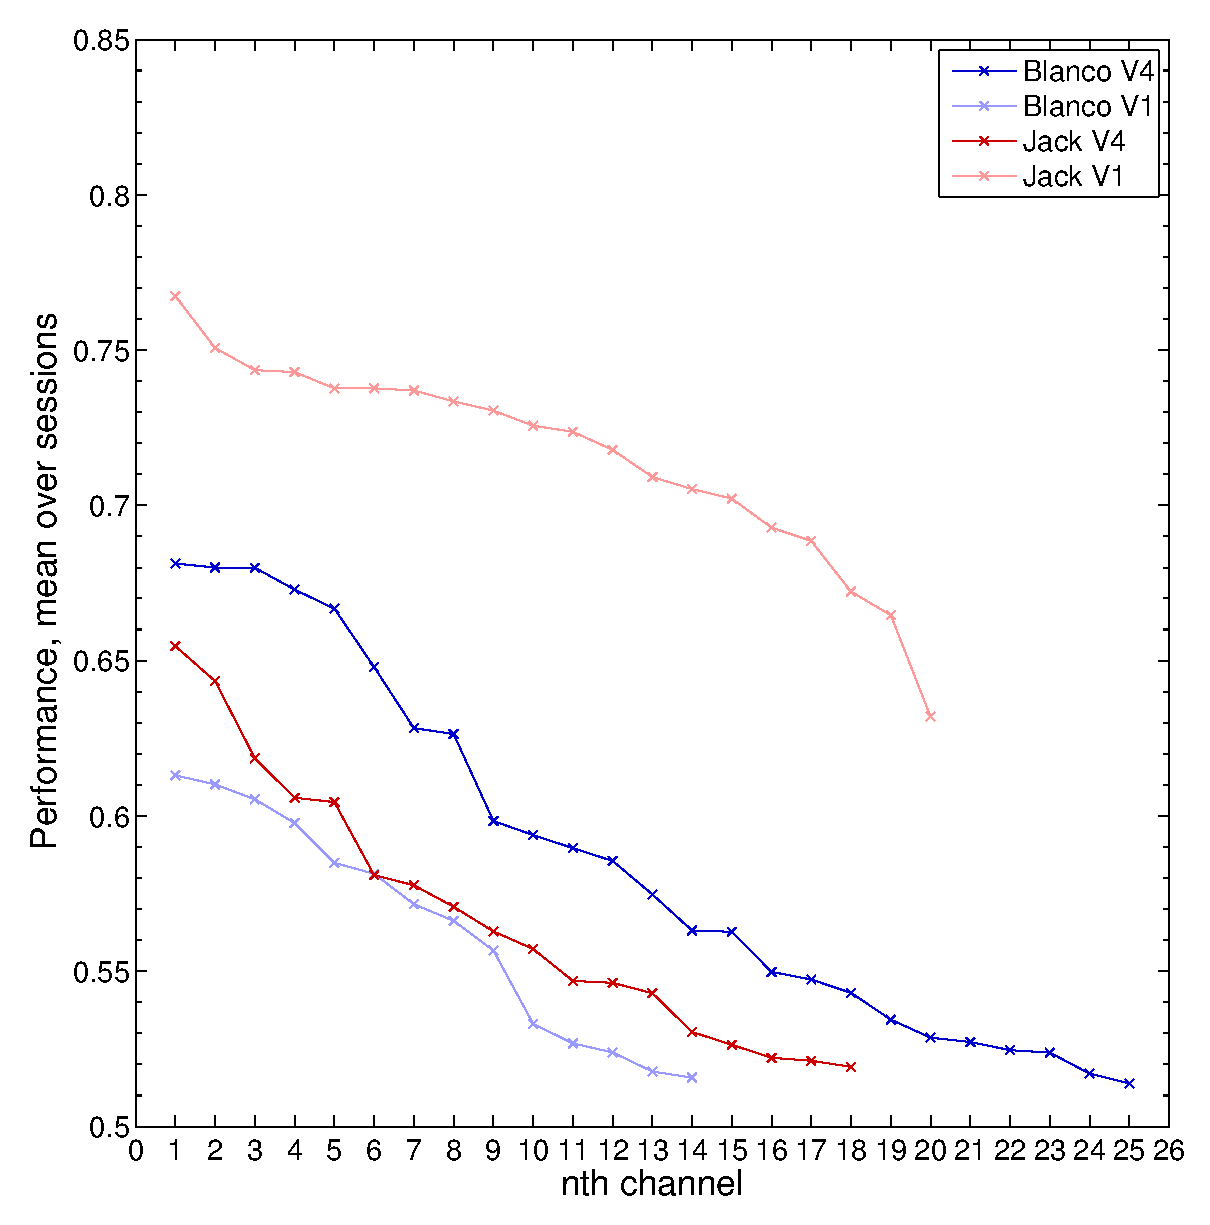
\includegraphics[width=\linewidth]{%
figs/decoding/2FC_singles.eps}
    \end{subfigure}
    ~~
    \begin{subfigure}[b]{0.5\linewidth}
        \centering
        \caption{}
        \label{fig:dec_nbest}
        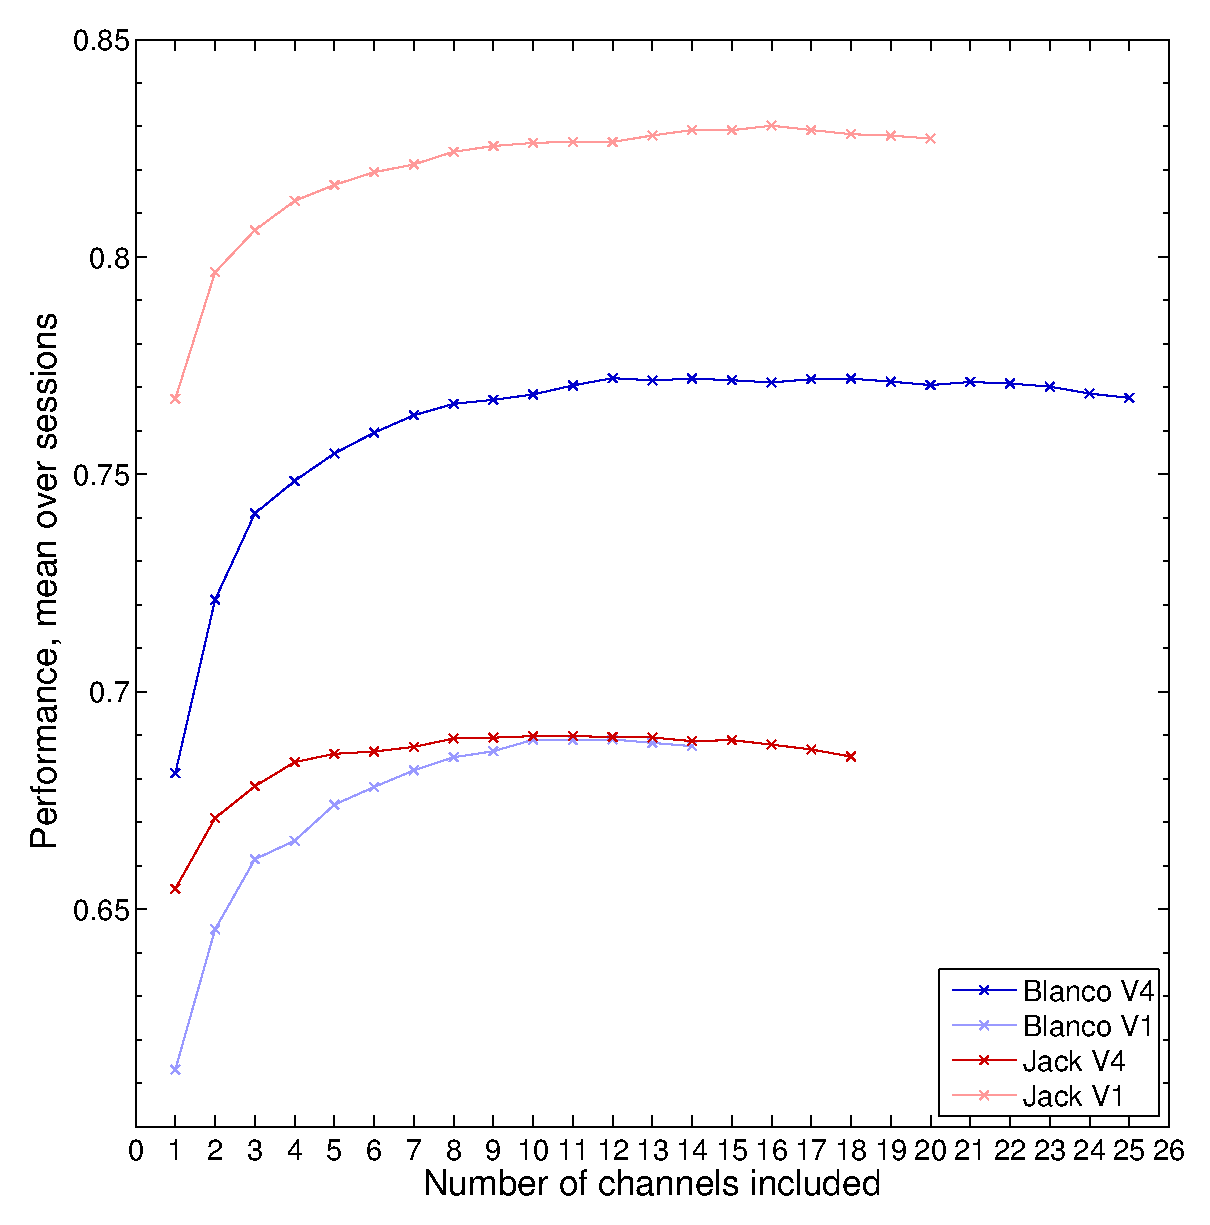
\includegraphics[width=\linewidth]{%
figs/decoding/2FC_nbest_all.eps}
    \end{subfigure}
    \caption{
\protect\subref{fig:dec_singles}: Distribution of decoder performance based on spike rate for individual channels, sorted by performance.
\protect\subref{fig:dec_nbest}: Decoding performance versus number of channels included in spiking data.
Channels were added one at a time, chosen so they maximise the decoder performance for that number of channels whilst keeping all the channels which had come before.
}
    \label{fig:dec_n}
\end{figure}

For each of the datasets, the performance decreases as the last 3 channels are added (Fig.~\ref{fig:dec_nbest}).
I speculate that this is because these channels only contain redundant information, and the increase in dimensionality decreases the quality of the classifier selected from the finite training data available.


\begin{figure}[htbp]
    \begin{subfigure}[b]{0.5\linewidth}
        \centering
        \caption{}
        \label{fig:dec_b4_allp}
	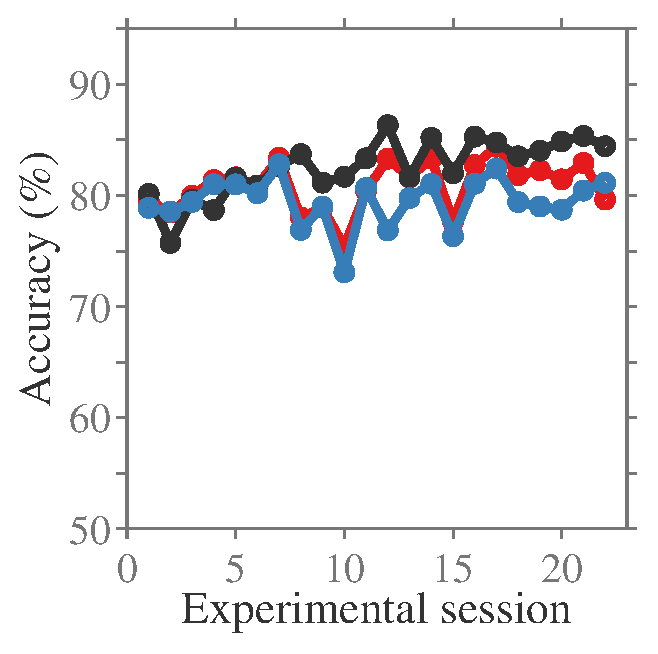
\includegraphics[width=\linewidth]{figs/decoding/perf_v4_blanco.eps}
    \end{subfigure}
    ~~
    \begin{subfigure}[b]{0.5\linewidth}
        \centering
        \caption{}
        \label{fig:dec_j4_allp}
	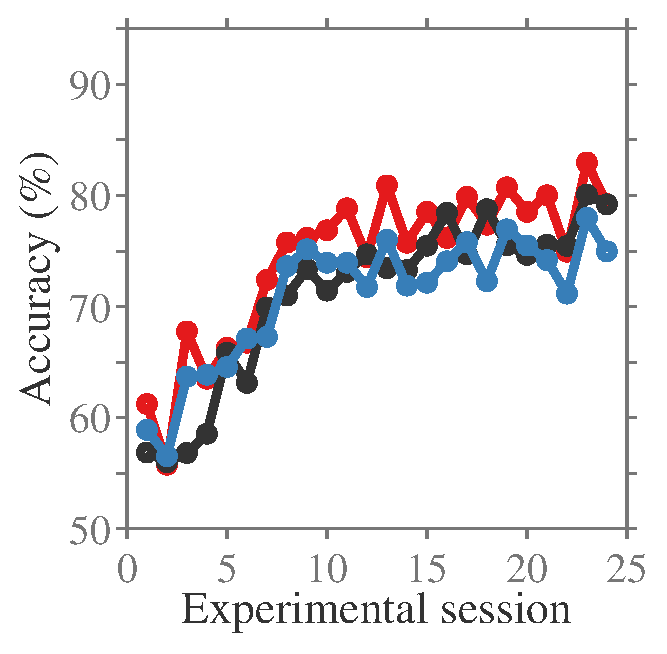
\includegraphics[width=\linewidth]{figs/decoding/perf_v4_jack.eps}
    \end{subfigure}
    \caption{%
    Decoding analysis for \ac{V4}.
    Performance of behavioural and decoding predictors by session, averaged across all conditions.
    Left panels: \ac{M1}. Right: \ac{M2}.
	Along the x-axis, `Session' is the animal's unique session ID, which increments by one for every day of training.
    On the y-axis, `proportion correct' is the proportion of trials for which the response is the same as the target.
    This is presented for behavioural performance (black), decoder performance (blue), and decoder performance when trials are shuffled, destroying noise correlations (red; see text).
}
    \label{fig:dec_all_v4}
\end{figure}

\begin{figure}[htbp]
    \begin{subfigure}[b]{0.5\linewidth}
        \centering
        \caption{}
        \label{fig:dec_b1_allp}
	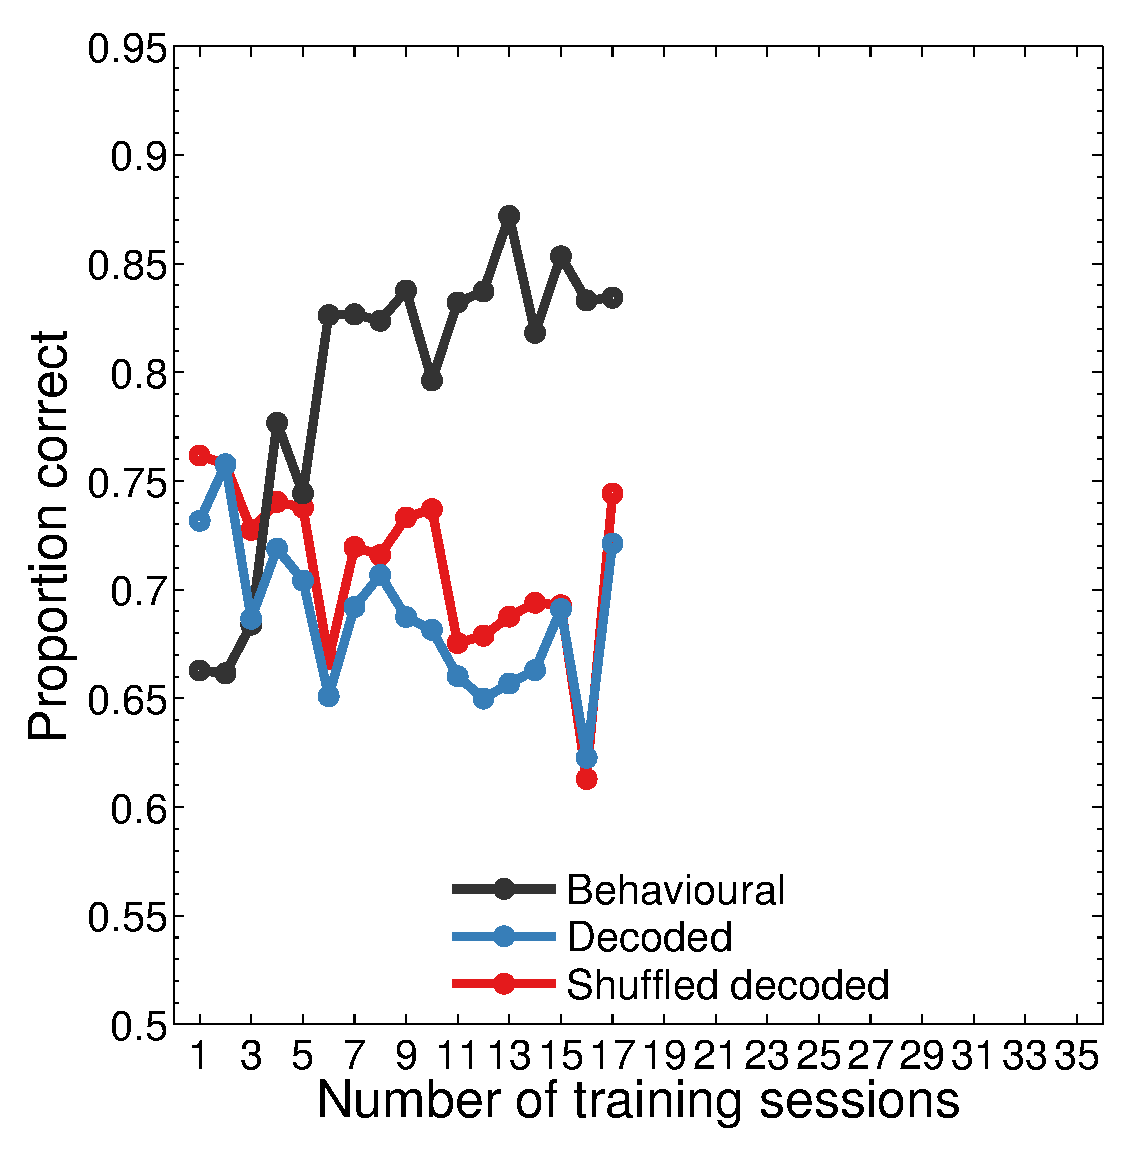
\includegraphics[width=\linewidth]{figs/decoding/perf_v1_blanco.eps}
    \end{subfigure}
    ~~
    \begin{subfigure}[b]{0.5\linewidth}
        \centering
        \caption{}
        \label{fig:dec_j1_allp}
	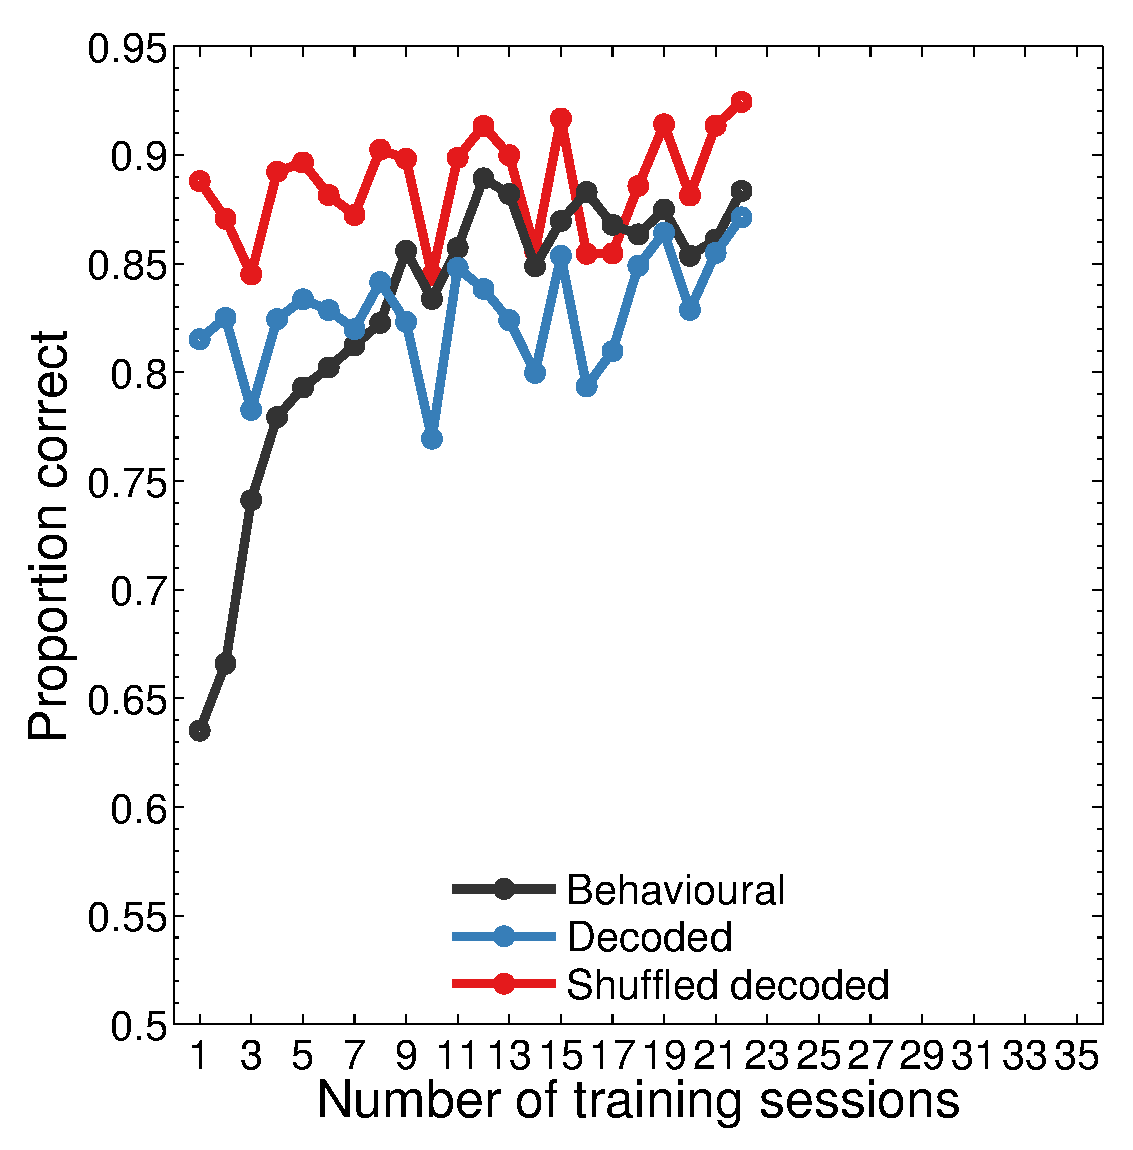
\includegraphics[width=\linewidth]{figs/decoding/perf_v1_jack.eps}
    \end{subfigure}
    \caption{%
    Decoding analysis for \ac{V1}.
    Performance of behavioural and decoding predictors by session, averaged across all conditions.
    Left panels: \ac{M1}. Right: \ac{M2}.
	Along the x-axis, `Session' is the animal's unique session ID, which increments by one for every day of training.
    On the y-axis, `proportion correct' is the proportion of trials for which the response is the same as the target.
    This is presented for behavioural performance (black), decoder performance (blue), and decoder performance when trials are shuffled, destroying noise correlations (red; see text).
}
    \label{fig:dec_all_v1}
\end{figure}



For \ac{M2} \ac{V4}, the trend in increase for behavioural performance is well matched by the change in performance of the decoder (Fig.~\ref{fig:dec_j4_allp}, blue and red lines).
In contrast to this, for \ac{M1} \ac{V4} we see the decoding performance is steady despite training, although it should be noted that the increase in behavioural performance was not so large for this animal.

For \ac{M2} \ac{V1}, there is a small gradual increase in decoder performance throughout training, though the increase does not match the timescales and rate of the increase in behavioural performance which is a much sharper transition.
Results for \ac{M2} \ac{V1} could be interpreted as indicating that no further improvements can be obtained from changes in \ac{V1}, and the behavioural performance is limited by the performance of the decoder.
For \ac{M1} \ac{V1}, there is a decrease in decoder in performance despite the increase in behavioural performance (Fig.~\ref{fig:dec_b1_allp}, blue and red lines respectively).


Shuffling the trials to destroy any noise correlations provides an improvement in performance for the data from \ac{M2}, indicating that noise correlations are detrimental to the successful decoding of stimuli.
However, there is no significant difference in decoder performance before and after shuffling for \ac{M1} datasets, which suggests noise correlations have no impact on decoding the contrast of stimuli using firing rate data from a population of neurons.
For \ac{M2} \ac{V1}, the benefit from shuffling seems to be reduced with training; the shuffled decoding performance is reasonably steady throughout training whilst the decoder with noise correlations included increases in performance, closing the gap.

% \marginnote{It might well be better to plot, for each area, the performances for both animals on the same plot and the expected vs observed behavioural agreement for both animals on a seperate plot.}


\begin{figure}[htbp]
    \begin{subfigure}[b]{0.5\linewidth}
        \centering
        \caption{}
        \label{fig:decag_b4_allp}
	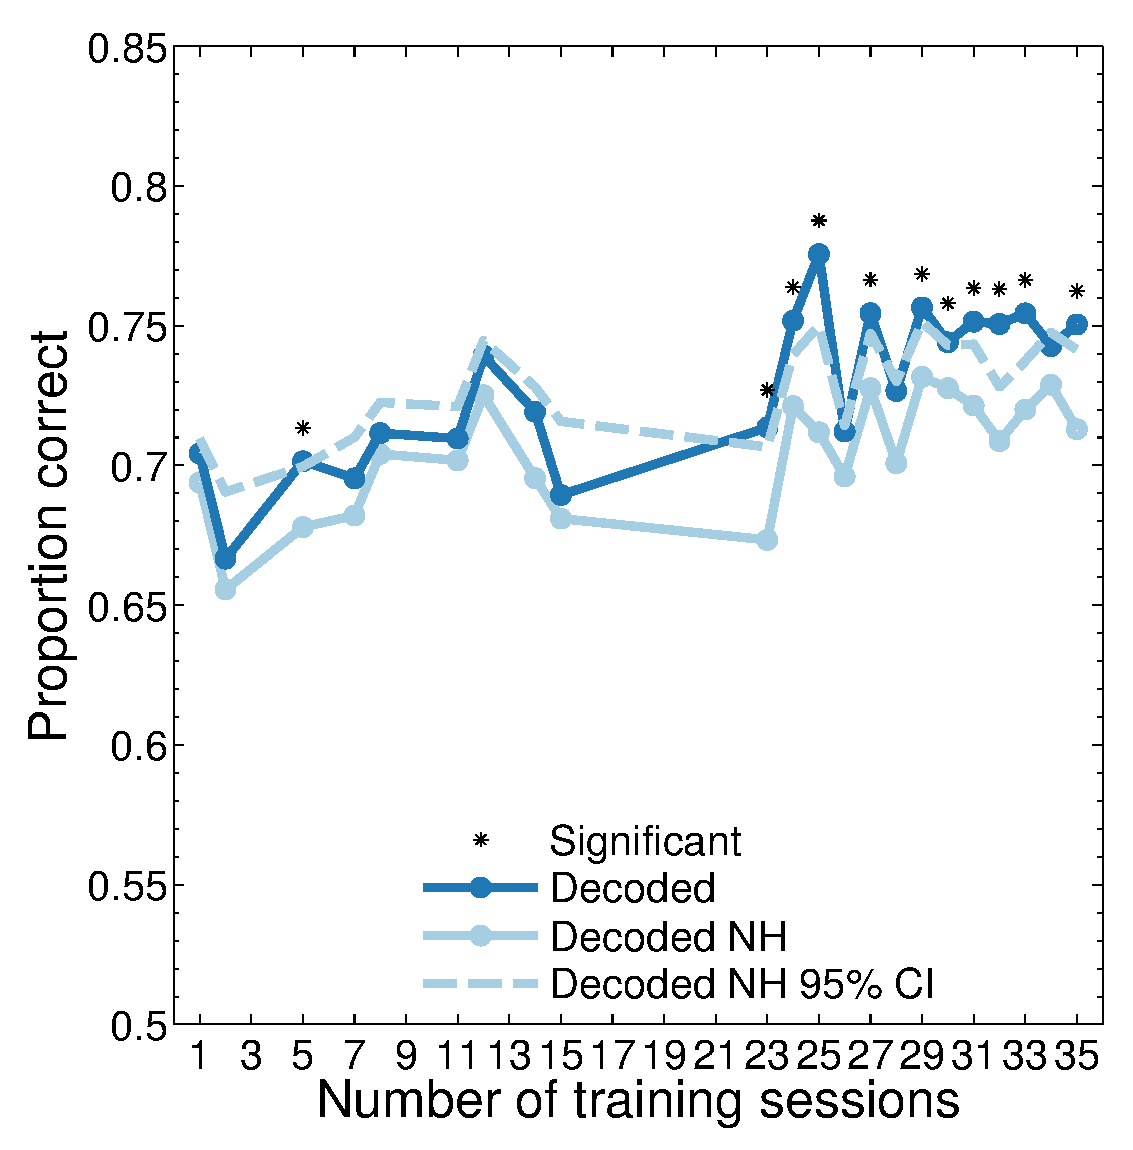
\includegraphics[width=\linewidth]{figs/decoding/agree_v4_blanco.eps}
    \end{subfigure}
    ~~
    \begin{subfigure}[b]{0.5\linewidth}
        \centering
        \caption{}
        \label{fig:decag_j4_allp}
	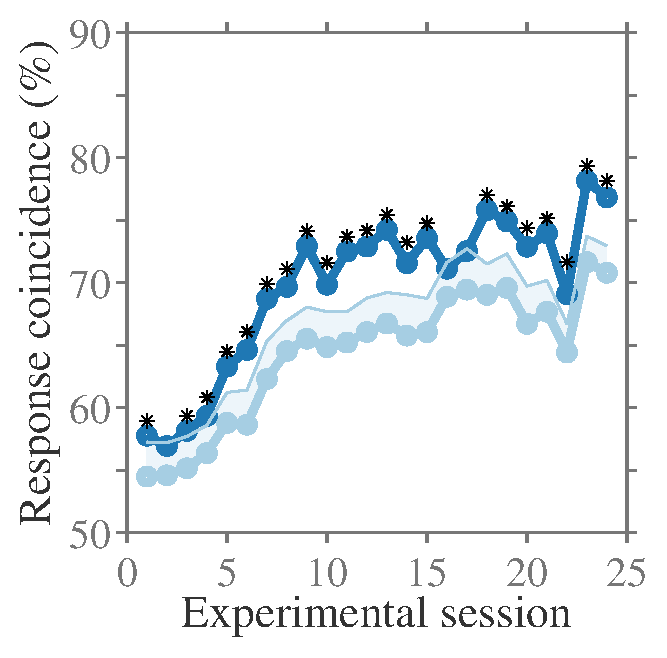
\includegraphics[width=\linewidth]{figs/decoding/agree_v4_jack.eps}
    \end{subfigure}
    \caption{%
    Decoding analysis for \ac{V4}.
    Trial-to-trial agreement between behavioural and decoding predictors.
    Left panels: \ac{M1}. Right: \ac{M2}.
	Along the x-axis, `Session' is the animal's unique session ID, which increments by one for every day of training.
    On the y-axis is the proportion of trials for which the response is the same as the behavioural response.
    The agreement between behaviour and decoding (unshuffled only) is presented alongside the null hypothesis of completely independent binomial distributions.
    The dashed line indicates the 95\% confidence interval of the null hypothesis.
}
    \label{fig:decag_all_v4}
\end{figure}

\begin{figure}[htbp]
    \begin{subfigure}[b]{0.5\linewidth}
        \centering
        \caption{}
        \label{fig:decag_b1_allp}
	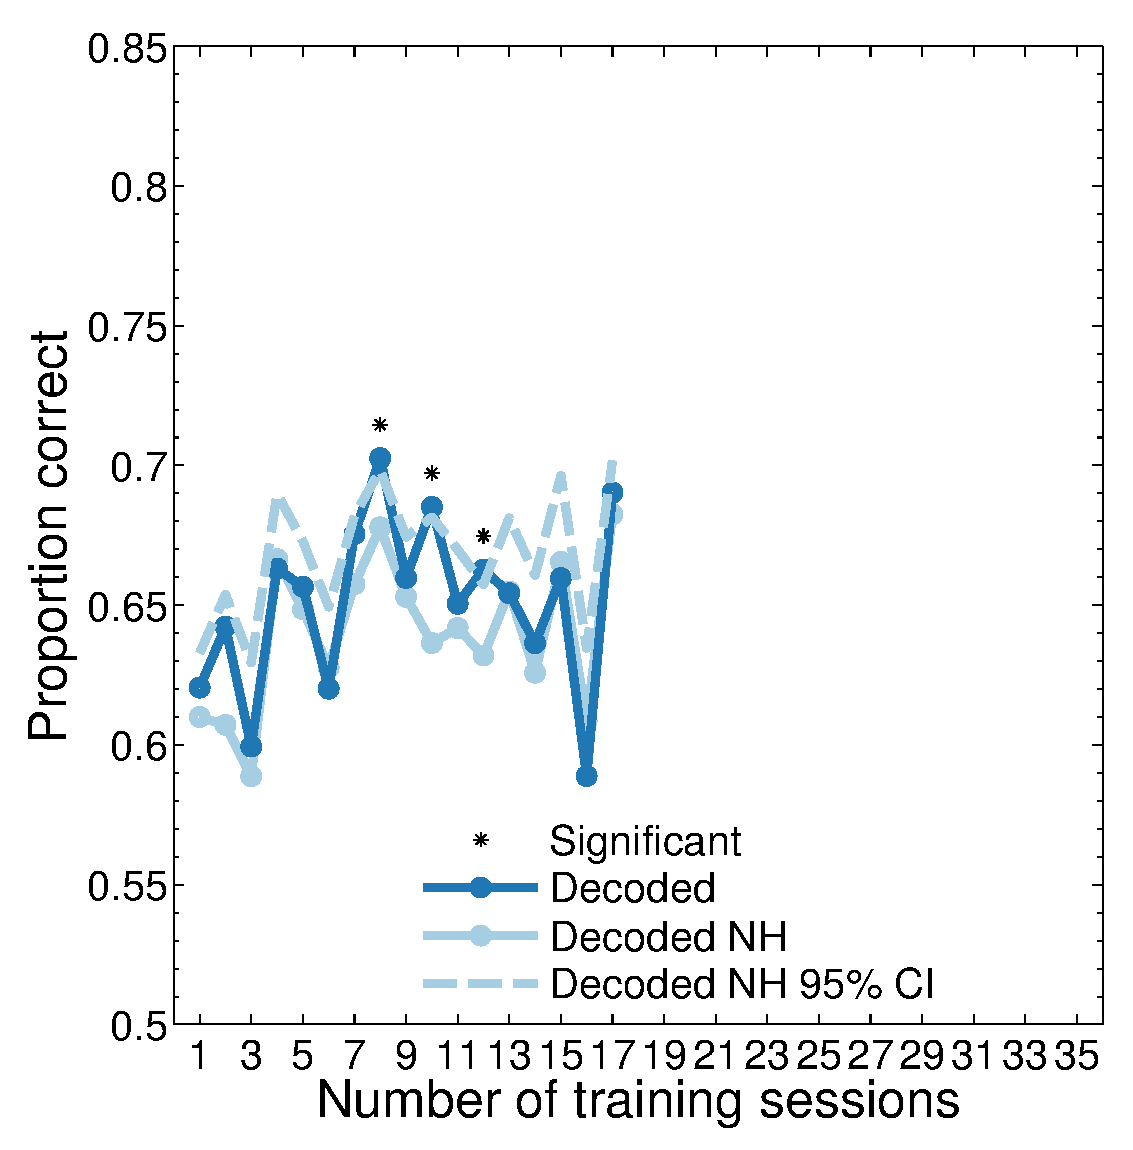
\includegraphics[width=\linewidth]{figs/decoding/agree_v1_blanco.eps}
    \end{subfigure}
    ~~
    \begin{subfigure}[b]{0.5\linewidth}
        \centering
        \caption{}
        \label{fig:decag_j1_allp}
	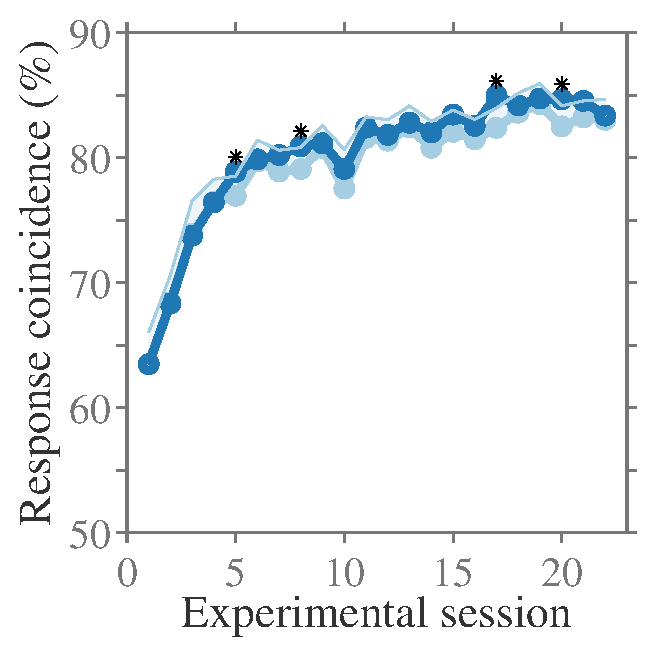
\includegraphics[width=\linewidth]{figs/decoding/agree_v1_jack.eps}
    \end{subfigure}
    \caption{%
    Decoding analysis for \ac{V1}.
    Trial-to-trial agreement between behavioural and decoding predictors.
    Left panels: \ac{M1}. Right: \ac{M2}.
	Along the x-axis, `Session' is the animal's unique session ID, which increments by one for every day of training.
    On the y-axis is the proportion of trials for which the response is the same as the behavioural response.
    The agreement between behaviour and decoding (unshuffled only) is presented alongside the null hypothesis of completely independent binomial distributions.
    The dashed line indicates the 95\% confidence interval of the null hypothesis.
}
    \label{fig:decag_all_v1}
\end{figure}


With regards to the behavioural and decoding response agreement, we find there is no consistent significant deviation from the null hypothesis for \ac{V1} data.
There are a couple of sessions where unshuffled agreement is above the boundary for significance for each of the animals, but this is not a consistent effect.
The agreement between shuffled decoding and behaviour does not deviate from the corresponding null hypothesis.
This shows that the shuffled is higher than the unshuffled decoding agreement only because the shuffled decoder is more accurate at matching the target response.

For \ac{V4}, we see that the agreement does not deviate significantly from the null hypothesis for earlier sessions, but after a cut off point all later sessions do (\ac{M1}: all sessions before 321 are not, after 329 are significant; \ac{M2}: Before 28 are not, after 28 are significant).
The effect is stronger for \ac{M2}, but present for both animals.
This indicates that the behavioural responses and the decoded responses based on the neural data were not notably correlated, but have become so with training.

Because the shuffled decoded responses are more accurate (with respect to the target response), they are predicted under the null hypothesis to be in better agreement with the behavioural responses.
However we observe these are in worse agreement than the unshuffled decoding, and do not deviate from the corresponding NH line.

A more detailed breakdown of these results with subsets of the 14 conditions is given in Figs.~\ref{fig:dec_detail_b1} and \ref{fig:dec_detail_j4}.
Comparing Figs.~\ref{fig:dec_b4_6easy_a} and \ref{fig:dec_j4_6easy_a} with Figs.~\ref{fig:dec_b4_6hard_a} and \ref{fig:dec_j4_6hard_a}, we can see that the decoding responses for the easier conditions fit the null hypothesis model, whilst the more challenging conditions do not and have a statistically significant agreement with the animal behaviour.


%==============================================================================
\FloatBarrier
\section{Information Theory-based methods}
%------------------------------------------------------------------------------

%------------------------------------------------------------------------------
\subsection{Session-based analysis}

The information was computed for each day of training (hereafter referred to as a session), for each of the channels from which recordings were available.
To gauge the typical behaviour of a neuron, the mean was taken over all the channels.
The mutual information between the spiking activity during test presentation and the identity of the test stimulus was computed
using a spike-timing based code.
This computation was done using the \verb|information| function from the freely available Information Break-down Toolbox \citep{Magri2009} for MATLAB.%
\footnote{Available at \url{http://www.ibtb.org}}

A moving window of $\SI{20}{ms}$ was taken and subdivided into 5 sequential bins, each of $\SI{4}{ms}$.
The number of spikes within each of the 5 bins was totalled up to provide a code letter for the bin.
The combination of the 5 sequential counts forms a codeword.

This is performed across all the trials in a session with the $\SI{20}{ms}$ window placed with the same offset relative to the test stimulus onset.
By assembling the trials according to their test contrast, the mutual information between the contrast and the spiking activity in this window can be computed.

Following the methods employed by the research group, only trials in which the monkey responded correctly were used for this analysis.

%------------------------------------------------------------------------------
% 5bins of 4ms
% figs/info/I_sessionwise_blanco_v1_chmean23_s343-359_oc1_5bins_of_4ms_dr_naive_pcolorhot_20120815T150057.png
% figs/info/I_sessionwise_blanco_v4_chmean31_s307,308,311,313,314,317,318,320,321,329-341_oc1_5bins_of_4ms_dr_naive_pcolorhot_20120815T150100.png
% figs/info/I_sessionwise_jack_v1_chmean25_s51-72_oc1_5bins_of_4ms_dr_naive_pcolorhot_20120815T150049.png
% figs/info/I_sessionwise_jack_v4_chmean20_s24-49_oc1_5bins_of_4ms_dr_naive_pcolorhot_20120815T150053.png
% 1 bin of 20ms
% figs/info/I_sessionwise_blanco_v1_chmean23_s343-359_oc1_1bins_of_20ms_dr_naive_pcolorhot_20120815T190833.png
% figs/info/I_sessionwise_blanco_v4_chmean31_s307,308,311,313,314,317,318,320,321,329-341_oc1_1bins_of_20ms_dr_naive_pcolorhot_20120815T190836.png
% figs/info/I_sessionwise_jack_v1_chmean25_s51-72_oc1_1bins_of_20ms_dr_naive_pcolorhot_20120815T190825.png
% figs/info/I_sessionwise_jack_v4_chmean20_s24-49_oc1_1bins_of_20ms_dr_naive_pcolorhot_20120815T190829.png
% 
% figs/info/I_sessionwise_blanco_v1_chmean23_s343-359_oc1_5bins_of_4ms_dr_naive_pcolorhot_20120815T202102.png
% figs/info/I_sessionwise_blanco_v4_chmean31_s307,308,311,313,314,317,318,320,321,329-341_oc1_5bins_of_4ms_dr_naive_pcolorhot_20120815T202106.png
% figs/info/I_sessionwise_jack_v1_chmean25_s51-72_oc1_5bins_of_4ms_dr_naive_pcolorhot_20120815T202053.png
% figs/info/I_sessionwise_jack_v4_chmean20_s24-49_oc1_5bins_of_4ms_dr_naive_pcolorhot_20120815T202058.png


%%\begin{figure}
%%\centering
%%\subfloat[A big tikz picture.\label{fig:one}]{%
%%  \makebox[\textwidth][l]{% %%% as above
%%  \resizebox{.45\largefigure}{!}{%
%%    \input{fig/tikzfile}}}}%
%%\hfill%
%%\subfloat[Another big tikz picture.\label{fig:two}]{%
%%  \makebox[\textwidth][l]{% %%% as above
%%  \resizebox{.45\largefigure}{!}{%
%%    \input{fig/tikzfile}}}}%
%%\caption{Two tikz pictures}
%%\label{fig:label}
%%\end{figure}
%%
%%\begin{figure}%
%%\centering
%%\subfloat[][]{...figure code...}%
%%\qquad
%%\subfloat[][]{...figure code...}%
%%\caption{Here are the first two figures of a continued figure.}%
%%\label{fig:cont}%
%%\end{figure}

% \begin{figure}[htbp]%
%     \centering
%     \subfloat[][\ac{M1} \ac{V1}.\label{fig:sessb1}]{%
%         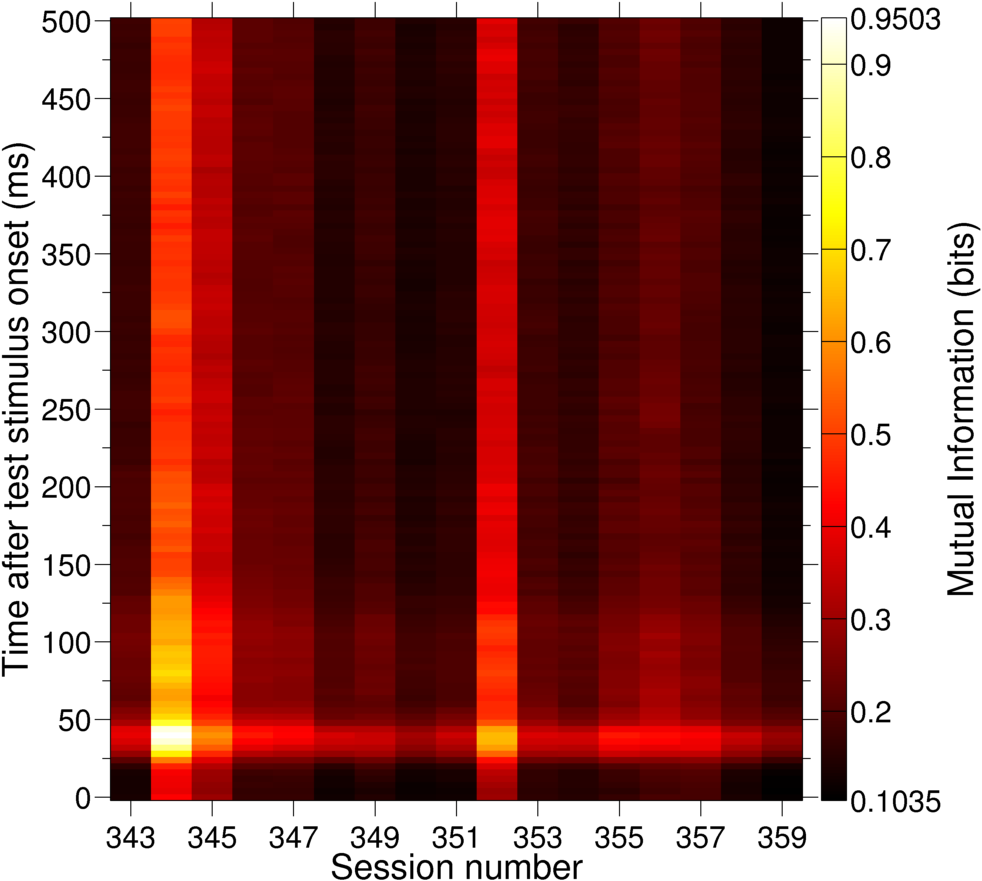
\includegraphics[scale=.25]{%
% figs/info/I_sessionwise_blanco_v1_chmean23_s343-359_oc1_5bins_of_4ms_dr_naive_pcolorhot_20120815T202102.png}
%     }%
%     ~~
%     \subfloat[][\ac{M1} \ac{V4}.\label{fig:sessb4}]{%
%         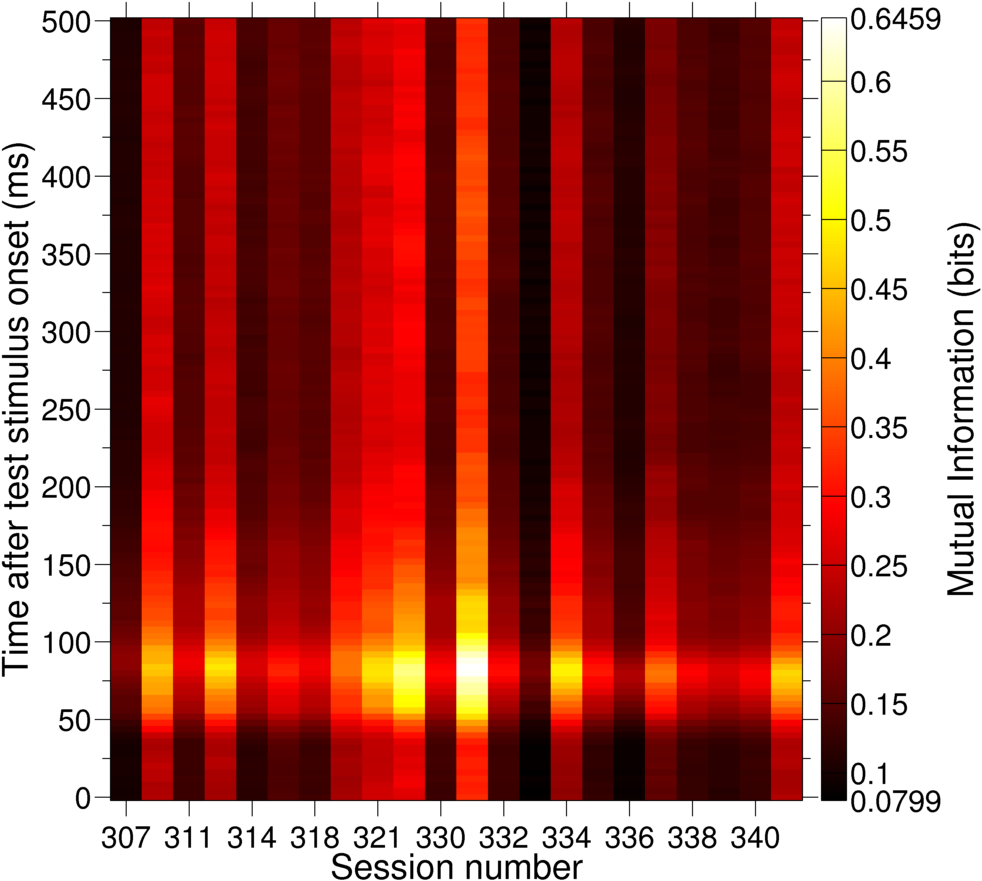
\includegraphics[scale=.25]{%
% figs/info/I_sessionwise_blanco_v4_chmean31_s307,308,311,313,314,317,318,320,321,329-341_oc1_5bins_of_4ms_dr_naive_pcolorhot_20120815T202106.png}
%     }%
%     \\
%     \subfloat[][\ac{M2} \ac{V1}.\label{fig:sessj1}]{%
%         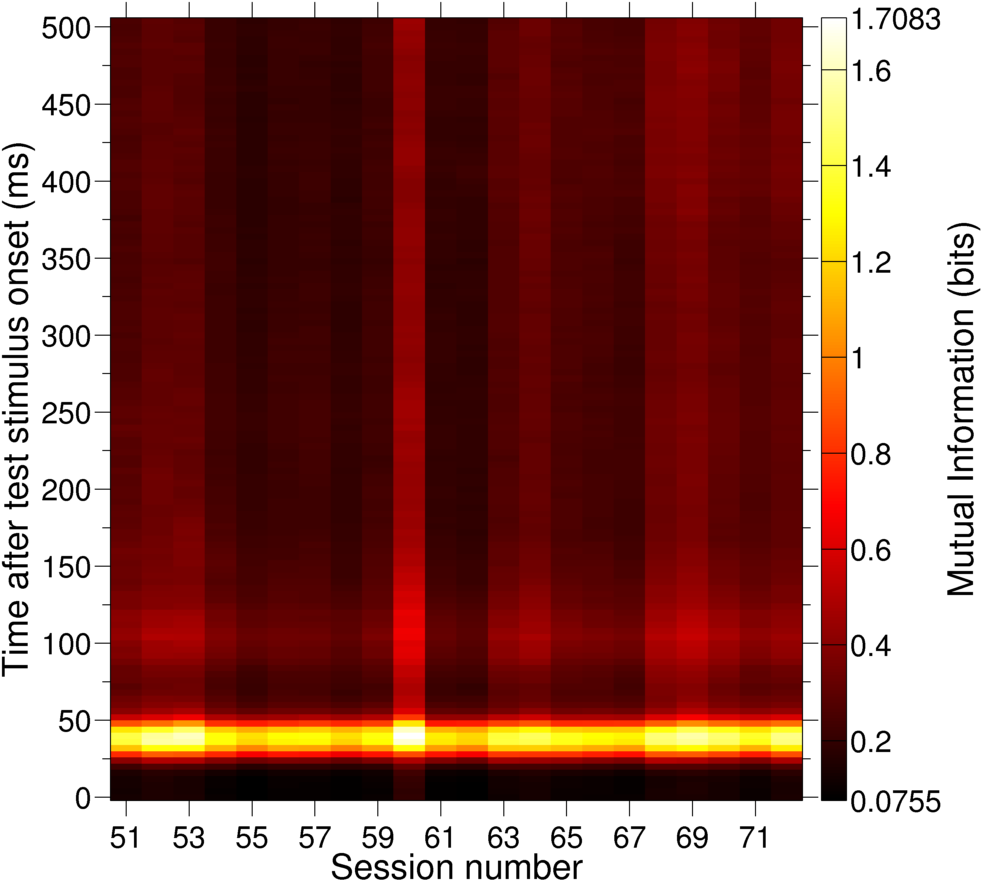
\includegraphics[scale=.25]{%
% figs/info/I_sessionwise_jack_v1_chmean25_s51-72_oc1_5bins_of_4ms_dr_naive_pcolorhot_20120815T202053.png}
%     }%
%     ~~
%     \subfloat[][\ac{M2} \ac{V4}.\label{fig:sessj4}]{%
%         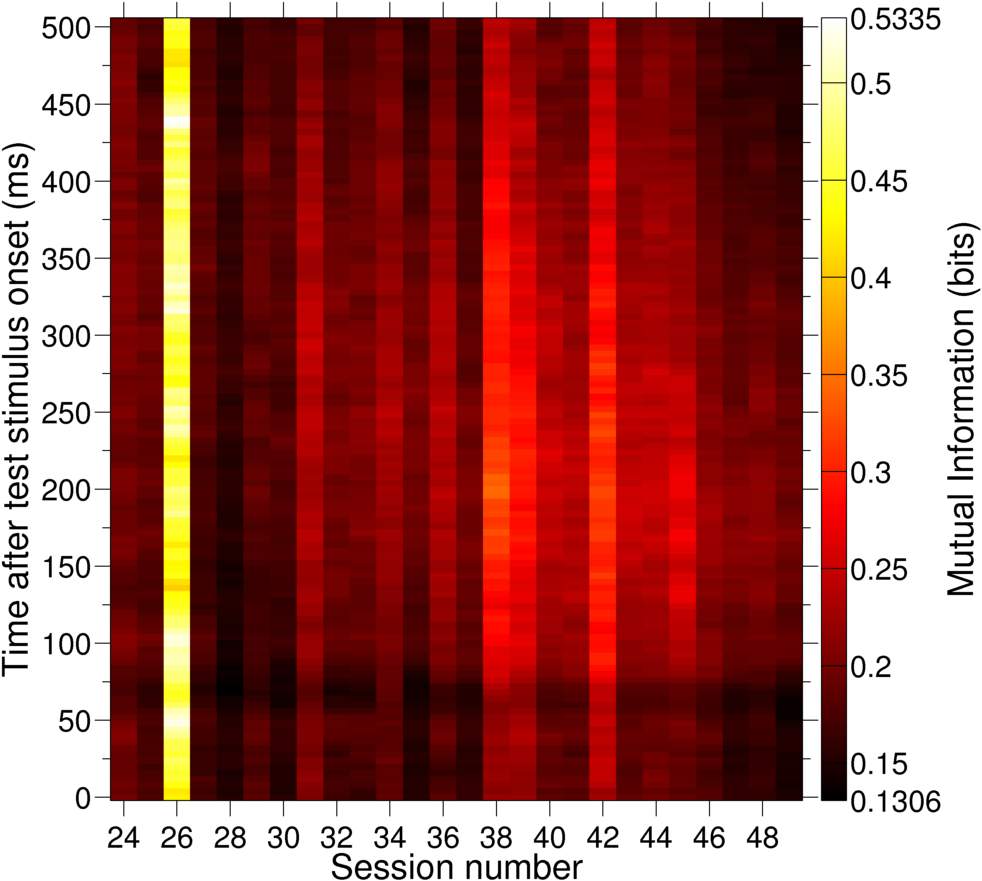
\includegraphics[scale=.25]{%
% figs/info/I_sessionwise_jack_v4_chmean20_s24-49_oc1_5bins_of_4ms_dr_naive_pcolorhot_20120815T202058.png}
%     }%
%     \caption{Mutual information between the test stimulus and the neural activity during test presentation.
% The mutual information with the test stimulus is taken for a spike timing based code for a \SI{20}{ms} window of spiking activity, sampled with the start of the window offset ($y$-axis) from \SI{0}{ms} up to \SI{500}{ms} after test stimulus onset (which is slightly more than \SI{20}{ms} before test stimulus offset).
% The sampling is in intervals of \SI{5}{ms}, so any 4 adjacent squares within each session are highly correlated.
% The recording session number for the data is given along the $x$-axis, and the number of days the animal has been trained for increases from left to right.
% Average mutual information across all the channels is denoted by the pseudo-colour of each of the rectangular patches, centred around the $(x,y)$ co-ordinate to which the measurement relates.
% In each case the average is taken across all available channel data: \ref{fig:sessb1}~23 channels, \ref{fig:sessb4}~30 channels, \ref{fig:sessj1}~25 channels, \ref{fig:sessj4}~20 channels.
% % The \ac{PT} bias correction method was used (see text).
% No bias correction method was used.
% }
%     \label{fig:sess}
% \end{figure}

% figs/info/I_sessionwise_blanco_v1_chmean23_s343-359_oc1_5bins_of_4ms_dr_pt_pcolorhot_20120811T130028.eps
% figs/info/I_sessionwise_blanco_v4_chmean31_s307,308,311,313,314,317,318,320,321,329-341_oc1_5bins_of_4ms_dr_pt_pcolorhot_20120811T130522.eps
% figs/info/I_sessionwise_jack_v1_chmean25_s51-72_oc1_5bins_of_4ms_dr_pt_pcolorhot_20120811T130003.eps
% figs/info/I_sessionwise_jack_v4_chmean20_s24-49_oc1_5bins_of_4ms_dr_pt_pcolorhot_20120811T133212.eps

The results of this initial analysis are shown in Fig.~\ref{fig:sess}.
% Although the relationship between different window offsets and the mutual information is similar for each of the sessions, the
No trend in information content with learning can be discerned because the measured mutual information content varies wildly from session-to-session.


% Demonstrate how this is dominated by the number of trials in the session, regardless of bias correction technique

% figs/info/ntrialsIbyNindiv_blanco_v1_dr_naive_20120812T164553.eps
% figs/info/ntrialsIbyNindiv_blanco_v4_dr_naive_20120812T164553.eps
% figs/info/ntrialsIbyNindiv_jack_v1_dr_naive_20120812T164553.eps
% figs/info/ntrialsIbyNindiv_jack_v4_dr_naive_20120812T164553.eps
%
% figs/info/ntrialsIandNindiv_blanco_v1_dr_naive_20120812T175154.eps
% figs/info/ntrialsIandNindiv_blanco_v4_dr_naive_20120812T175154.eps
% figs/info/ntrialsIandNindiv_jack_v1_dr_naive_20120812T175154.eps
% figs/info/ntrialsIandNindiv_jack_v4_dr_naive_20120812T175154.eps
%
% figs/info/ntrialsIandNindiv_blanco_v1_dr_naive_1bins_of_20ms_20120815T200333.eps
% figs/info/ntrialsIandNindiv_blanco_v4_dr_naive_1bins_of_20ms_20120815T200333.eps
% figs/info/ntrialsIandNindiv_jack_v1_dr_naive_1bins_of_20ms_20120815T200333.eps
% figs/info/ntrialsIandNindiv_jack_v4_dr_naive_1bins_of_20ms_20120815T200333.eps
% 
% figs/info/ntrialsIandNindiv_blanco_v1_dr_naive_5bins_of_4ms_20120815T201856.eps
% figs/info/ntrialsIandNindiv_blanco_v4_dr_naive_5bins_of_4ms_20120815T201856.eps
% figs/info/ntrialsIandNindiv_jack_v1_dr_naive_5bins_of_4ms_20120815T201856.eps
% figs/info/ntrialsIandNindiv_jack_v4_dr_naive_5bins_of_4ms_20120815T201856.eps
% 
\begin{figure}[htbp]
    \begin{subfigure}[b]{0.5\linewidth}
        \centering
        \caption{\ac{M1} \ac{V1}}
        \label{fig:IandNb1}
        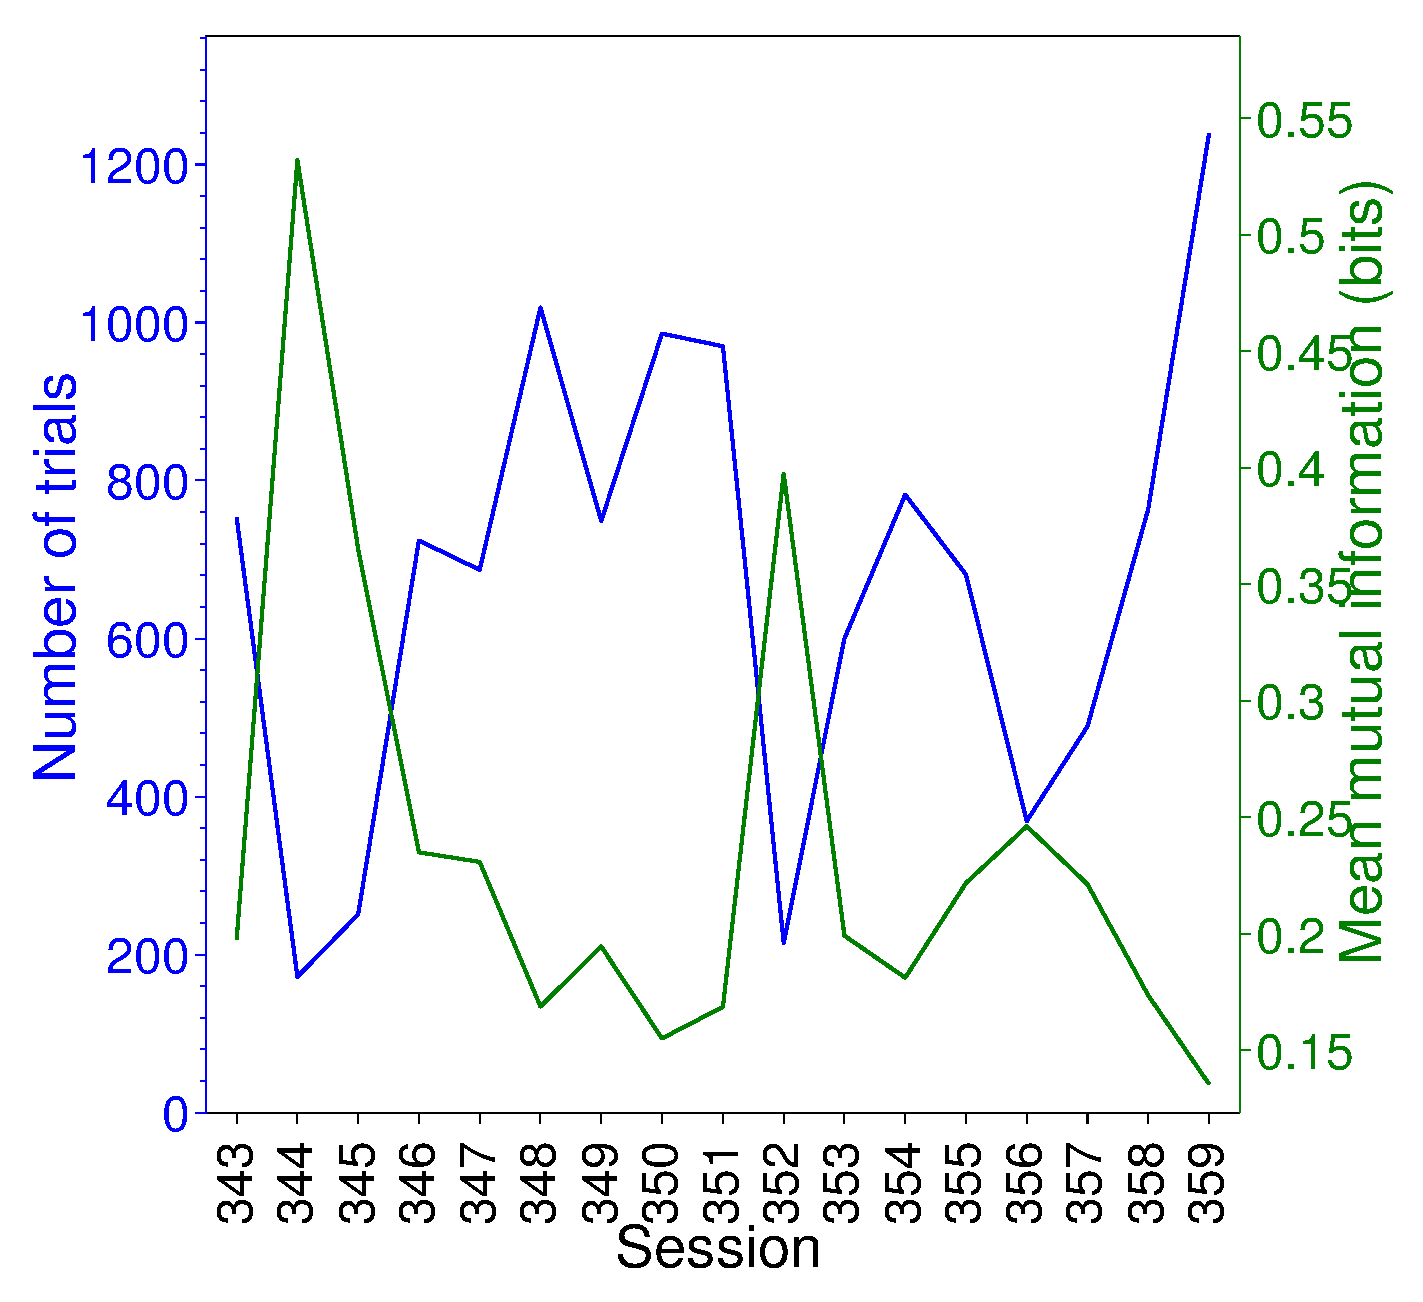
\includegraphics[width=\linewidth]{%
figs/info/ntrialsIandNindiv_blanco_v1_dr_naive_5bins_of_4ms_20120815T201856.eps}
    \end{subfigure}
    \begin{subfigure}[b]{0.5\linewidth}
        \centering
        \caption{\ac{M1} \ac{V4}}
        \label{fig:IandNb4}
        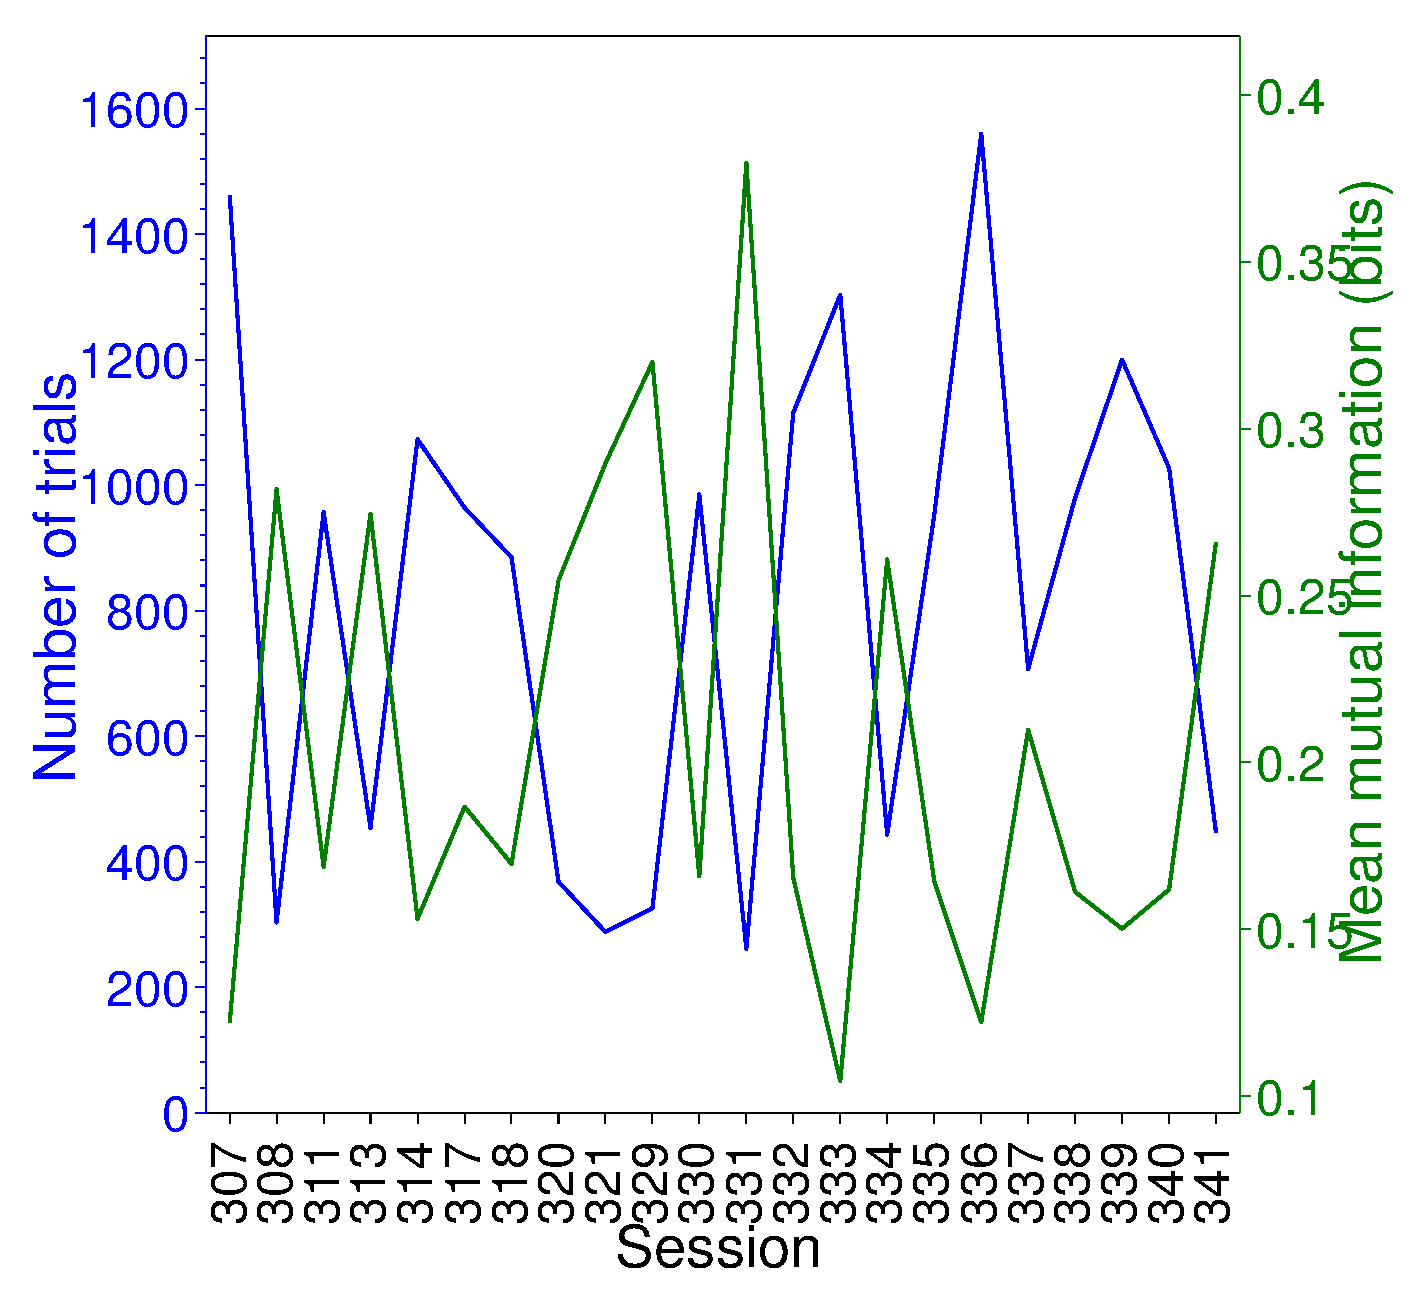
\includegraphics[width=\linewidth]{%
figs/info/ntrialsIandNindiv_blanco_v4_dr_naive_5bins_of_4ms_20120815T201856.eps}
    \end{subfigure}
    \\
    \begin{subfigure}[b]{0.5\linewidth}
        \centering
        \caption{\ac{M2} \ac{V1}}
        \label{fig:IandNj1}
        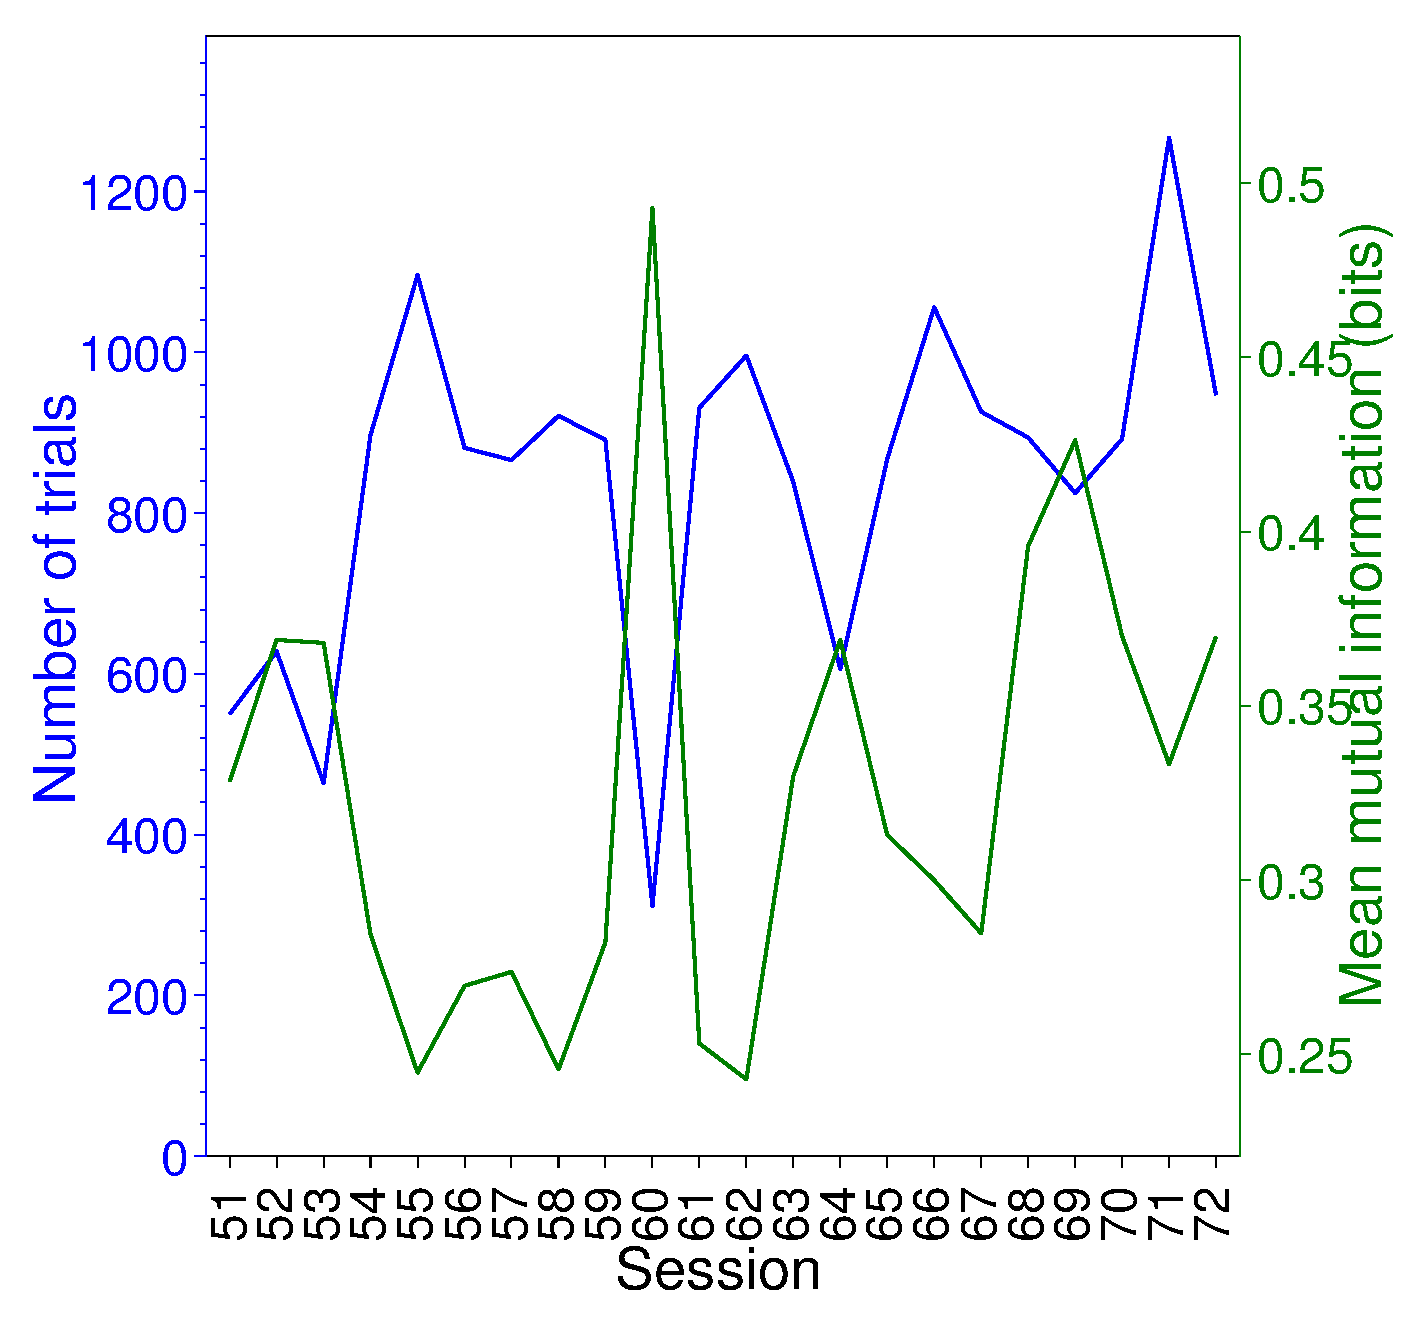
\includegraphics[width=\linewidth]{%
figs/info/ntrialsIandNindiv_jack_v1_dr_naive_5bins_of_4ms_20120815T201856.eps}
    \end{subfigure}
    \begin{subfigure}[b]{0.5\linewidth}
        \centering
        \caption{\ac{M2} \ac{V4}}
        \label{fig:IandNj4}
        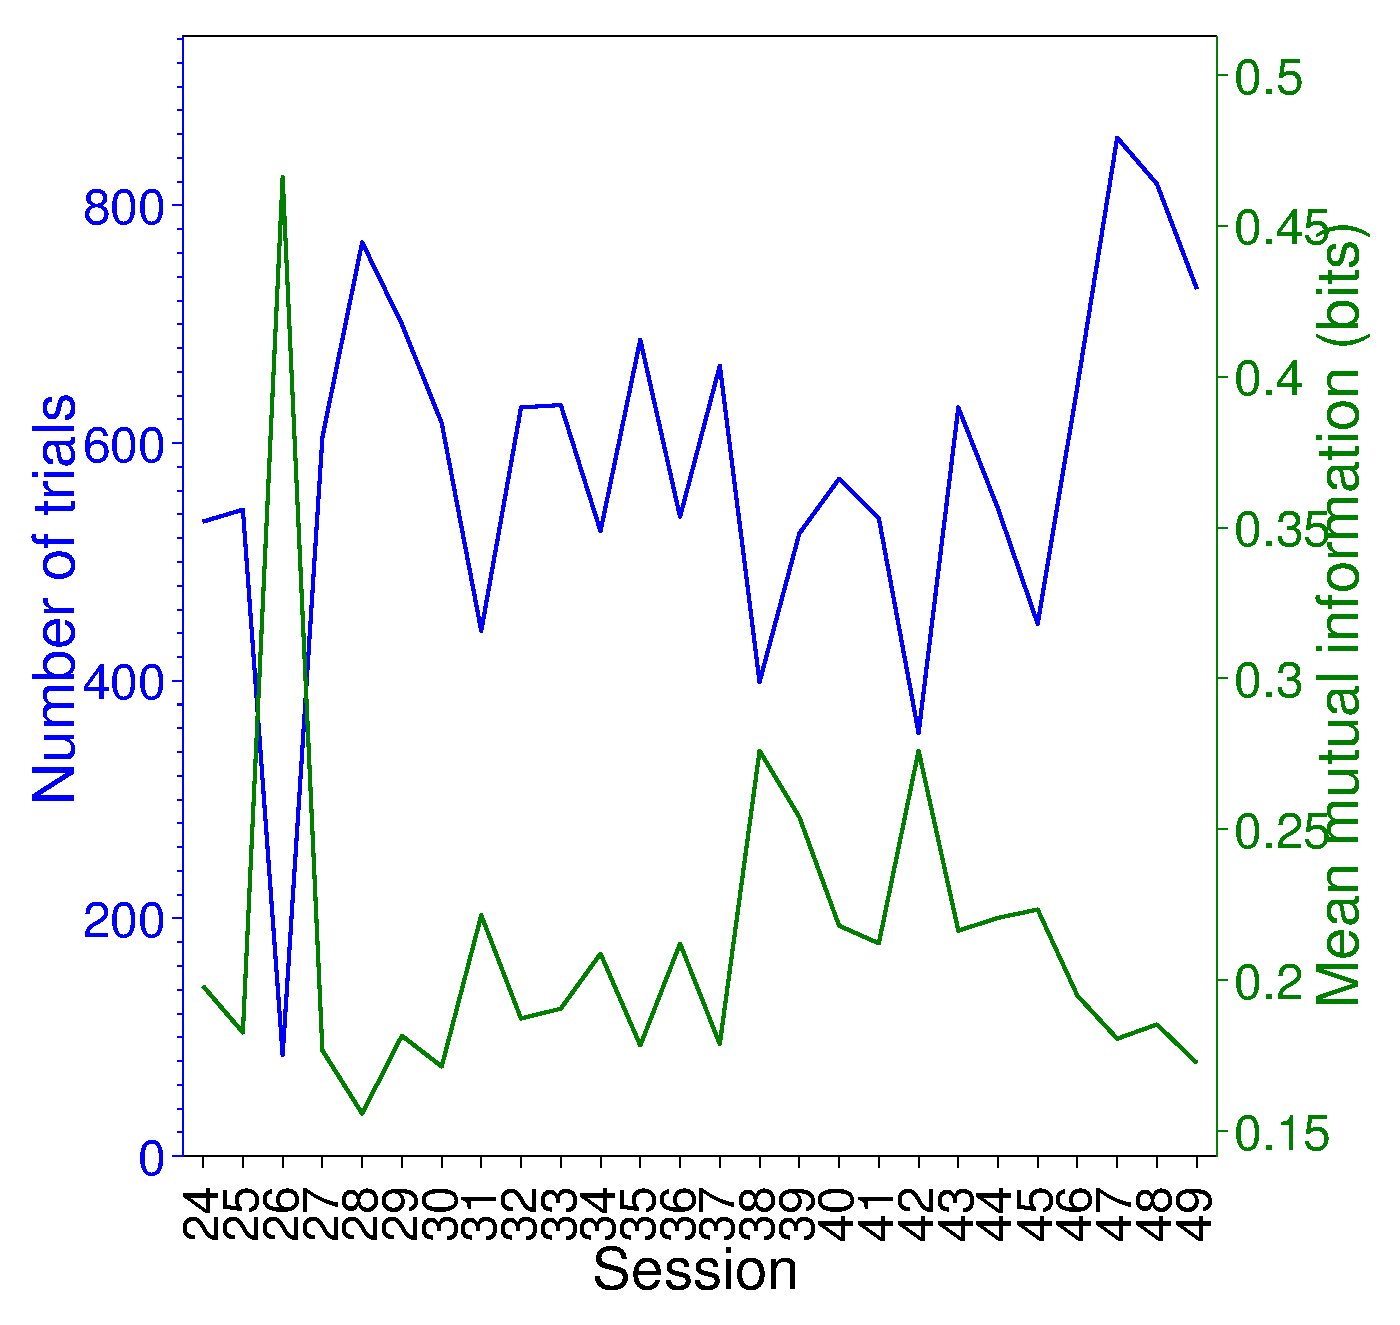
\includegraphics[width=\linewidth]{%
figs/info/ntrialsIandNindiv_jack_v4_dr_naive_5bins_of_4ms_20120815T201856.eps}
    \end{subfigure}
    \caption{Mutual information seems to be anti-correlated with the number of trials in the session. The number of correctly responded trials in each session is plotted on top of the mean information in individual sessions. The mutual information was not corrected for bias, and averaged across the whole period of test stimulus presentation.
%There is a missing data point for \ac{M2} \ac{V4} because in one session there were not enough trials per condition for the \ac{QE} algorithm to function.
}
    \label{fig:IandN}
\end{figure}

Fig.~\ref{fig:IandN} shows that the changes in the measured mutual information are dominated by the number of trials in the session, not by increases with perceptual learning (corresponding to increments in the session number).
The only exception to this rule seems to be for \ac{M2} \ac{V1}, shown in Fig.~\ref{fig:IandNj1}, where the information increases with learning despite an increase in the number of trials per session over this period.

% figs/info/ntrialsIvsinvNcombindiv_blanco_v1_20120812T164553.eps
% figs/info/ntrialsIvsinvNcombindiv_blanco_v4_20120812T164553.eps
% figs/info/ntrialsIvsinvNcombindiv_jack_v1_20120812T164553.eps
% figs/info/ntrialsIvsinvNcombindiv_jack_v4_20120812T164553.eps
% 
% figs/info/ntrialsIvsinvNcombindiv_blanco_v1_5bins_of_4ms_20120815T204808.eps
% figs/info/ntrialsIvsinvNcombindiv_blanco_v4_5bins_of_4ms_20120815T204808.eps
% figs/info/ntrialsIvsinvNcombindiv_jack_v1_5bins_of_4ms_20120815T204808.eps
% figs/info/ntrialsIvsinvNcombindiv_jack_v4_5bins_of_4ms_20120815T204808.eps
% 
\begin{figure}[htbp]
    \begin{subfigure}[b]{0.5\linewidth}
        \centering
        \caption{\ac{M1} \ac{V1}}
        \label{fig:IvNb1}
        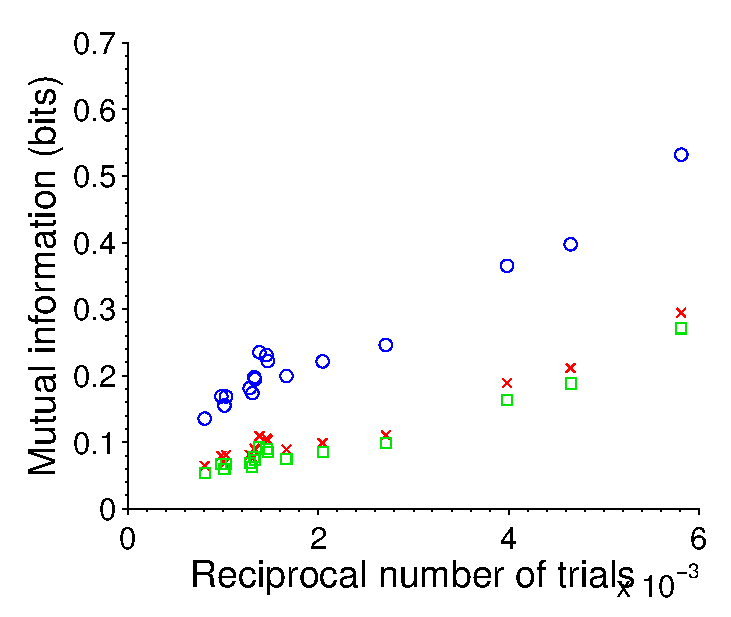
\includegraphics[width=\linewidth]{%
figs/info/ntrialsIvsinvNcombindiv_blanco_v1_5bins_of_4ms_20120815T204808.eps}
    \end{subfigure}
    \begin{subfigure}[b]{0.5\linewidth}
        \centering
        \caption{\ac{M1} \ac{V4}}
        \label{fig:IvNb4}
        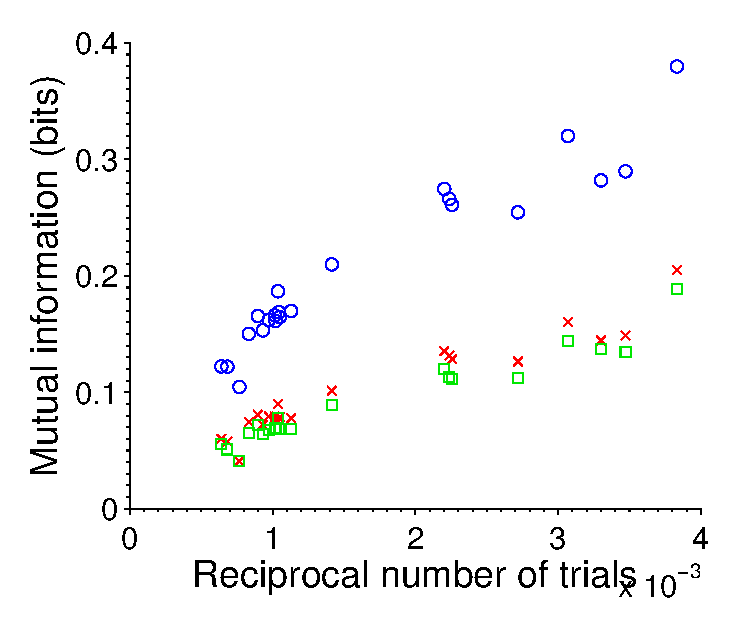
\includegraphics[width=\linewidth]{%
figs/info/ntrialsIvsinvNcombindiv_blanco_v4_5bins_of_4ms_20120815T204808.eps}
    \end{subfigure}
    \\
    \begin{subfigure}[b]{0.5\linewidth}
        \centering
        \caption{\ac{M2} \ac{V1}}
        \label{fig:IvNj1}
        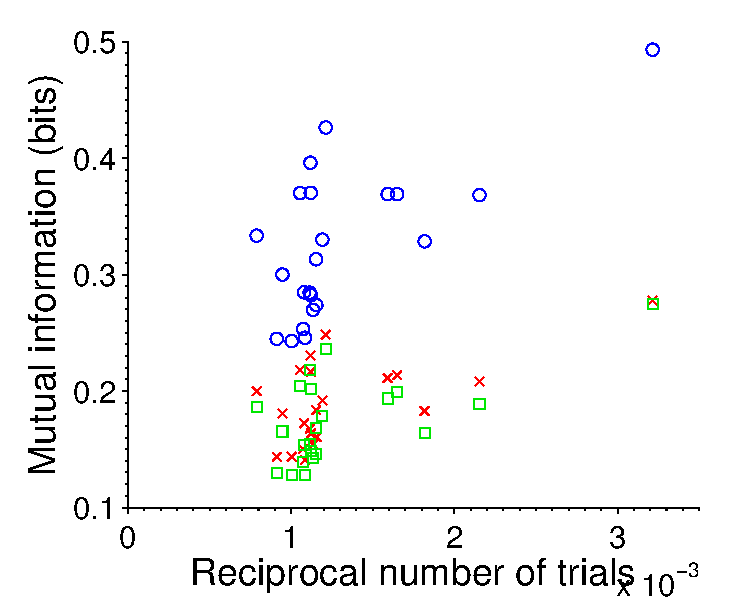
\includegraphics[width=\linewidth]{%
figs/info/ntrialsIvsinvNcombindiv_jack_v1_5bins_of_4ms_20120815T204808.eps}
    \end{subfigure}
    \begin{subfigure}[b]{0.5\linewidth}
        \centering
        \caption{\ac{M2} \ac{V4}}
        \label{fig:IvNj4}
        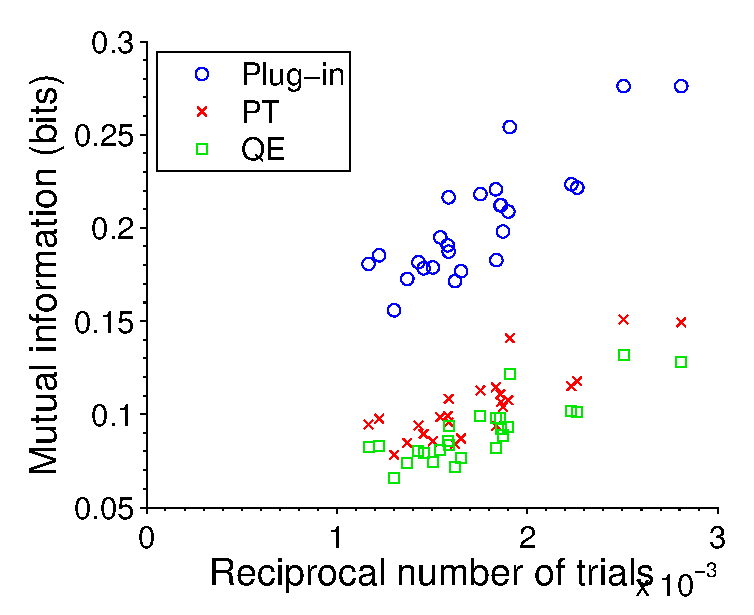
\includegraphics[width=\linewidth]{%
figs/info/ntrialsIvsinvNcombindiv_jack_v4_5bins_of_4ms_20120815T204808.eps}
    \end{subfigure}
    \caption{Mutual information is inversely correlated with the number of trials in the session. The mutual information for a single session is averaged over all channels, and averaged over all times during stimulus presentation, and plotted against the reciprocal of the number of trials in the session ($\nicefrac{1}{N}$). Plug-in:~without bias correction. \ac{PT}:~using the Panzeri-Treves method to correct for bias \citep{Panzeri1996}. \ac{QE}:~using quadratic extrapolation for bias correction \citep{Strong1998}.
%There is a missing data point for \ac{M2} \ac{V4} because in one session there were not enough trials per condition for the \ac{QE} algorithm to function.
}
    \label{fig:IvN}
\end{figure}

In particular, the measured value for the mutual information is strongly correlated with the reciprocal of the number of trials in the session (Fig.~\ref{fig:IvN}).
The correlation is still very strong even if we use one of the two bias correction techniques.
As discussed above, for \ac{M2} \ac{V1} the number of trials per session and the measured information  are both correlated with time, which reduces the correlation observed in Fig.~\ref{fig:IvNj1}.

The problem is that although \ac{PT} and \ac{QE} both do a reasonable attempt at removing the bias, they are not perfect and some bias will remain.
As the bias is dependent on the number of trials, it is unsurprising the remaining bias follows the same dependency.
In particular, in the asymptotic regime the leading term in the expansion of $I_{\text{measured}}$ is known to be proportional \citep{Treves1995} to $\nicefrac{1}{N}$; the same relationship observed here.

In particular, the difficult faced is changes due to perceptual learning which are of interest may only be slight, but the the number of trials per session varies five-fold: from 250 up to 1250.
Consequently it is unsurprising that the observed differences in information day-to-day are dominated by the number of trials.

%------------------------------------------------------------------------------
\subsection{Trial-based analysis}

To counter the correlation between measured information and number of trials, an obvious solution is to use the same number of trials for every computation.
We now consider how many trials should be taken at once to obtain a reasonably reliable estimate.

Some rules-of-thumb for the number of trials are offered by \citep{Panzeri2007}.
Let $\overline{R}$ denote the number of possible response codes.
Then, for the bias-uncorrected estimate of mutual information, we need to have at least $N_S \ge 2^{32} \, \overline{R}$ trials per stimulus,
whilst if the \ac{PT} or \ac{QE} bias correction methods are applied, we only need $N_S > 2 \, \overline{R}$.

% The spike detection software was set to only detect spikes at least \SI{3}{ms} apart, and moreover, 
The probability of having two spikes within \SI{4}{ms} from a non-bursting neuron is very low.
For example, a neuron with a high firing rate might fire at \SI{100}{Hz}, which means inter-spike intervals are typically around \SI{10}{ms} (and \SI{100}{Hz} is a high firing rate for the channels in our dataset).
Consequently any \SI{4}{ms} bin will realistically contain either 0 or 1 spikes, and the number of possible response codes in our spike timing code analysis with 5 bins each of \SI{4}{ms} is $\overline{R} = 2^5 = 32$.
In comparison for a spike count code, if we assume spikes cannot be closer together than \SI{3}{ms}, there are between 0 and 7 spikes in any \SI{20}{ms} interval.
Consequently there are $\overline{R} = 8$ possible response codes.

As we wish our analysis to work for both spike timing and spike count codes, using the above rules we need to use at least 64 trials per stimulus to get a reasonable estimate of the information with one of the bias correction methods in place.
Since there are 14 different stimuli, this means at least 896 trials in total are needed.
This presents a dilemma, since most of the sessions are shorter than this, even when both correctly and incorrectly responded trials are included.
Excluding sessions with fewer than 896 trials would severely limit the size of the dataset.
% and the patchwork of holes which would result would limit how much can be read into the results due to  which would result.

The solution found was to concatenate the sessions together and analyse groups of $N$ trials taken from multiple consecutive sessions.
The na\"{i}ve justification for this approach is a ``first-order approximation'' to perceptual learning would be that the monkey gets better at recognising the stimuli every-time they perceive it, and so the most important quantifier for the amount of perceptual learning which has taken place is the total number of trials the monkey has performed to date.

This rather basic assumption neglects several factors which influence the animal's performance, such as their mood during the particular training day; and factors which influence the animal's willingness to work (in turn influencing performance), which depends on their recent level of access to water (the reward used in the study).
For instance, the animal performs less well on Mondays, which follows on from readily available water during the weekend.
Furthermore, the consolidation which occurs during sleep is commonly believed to be important to perceptual learning, and (as this only occurs between training sessions) this effect is completely ignored by this approach.

However, the session-concatenation approach was attempted regardless, and a value of $N_S = 100$ trials per stimulus was chosen.
Though there are enough trials available to use more and reduce the bias further, it is undesirable data from so many sessions at once.

As mentioned in Chap.~\ref{ch:exp}, a delayed repeat is used for any trials to which the animal does not correctly respond.
Consequently, more difficult test stimuli (with contrasts close to the sample contrast) are presented significantly more frequently than easier stimuli.
For instance, when presented with the most difficult test stimuli, the animal will have a success rate only just above \SI{50}{\percent} on the first day of the experiment, rising to around \SI{70}{\percent} by the last day.
For the easiest stimuli, the success rate will be nearly \SI{100}{\percent} throughout.

Say we arrange all the trials into groups based on their stimulus, then take 100 subsequent trials from each of the groups to perform the analysis on.
Due to the different number of trials per stimulus, it will not be long before the trials selected for each stimulus are from very different points in time and from different sessions.\footnote{Even if we only analyse the correctly responded trials, there is still a difference in the number of trials per stimulus due to a limit on the number of repeats of any test condition.
The difference was negligible for \ac{M1}, but accumulated to a 100 trial difference over all the sessions between the most and least correctly responded conditions for \ac{M2}.}
To ensure all the trials are from when the animal has had the same amount of training, we can instead take a group of $S \cdot N_S = 14 \cdot 100 = 1400$ consecutive trials regardless of the stimulus presented and analysed.
The differences in number of trials per stimulus are not particularly important, so long as there are always  enough.

All trials where the monkey completed the trial and gave a response (either correct or incorrect) were included in the analysis.
Trials where the monkey did not complete the task by fixating and then providing a response as required were excluded.
Using both the correct and incorrectly responded trials means our distribution for $P(s)$ is the same as that presented to the monkey, and there are notably more trials available to perform the analysis on.

% Using 50 and 100 trials explored: not considerable difference between results. 100 shown for conciseness


%------------------------------------------------------------------------------
\subsection{General Information plots}

Starting with \ac{V1}, the first thing which is noticed in Figs.~\ref{fig:b1-trialwise} and \ref{fig:j1-trialwise} \ref{fig:b1-1x20tp4} and \ref{fig:b1-5x4tp4} is the large peak in information over the \SI{20}{ms} window starting at around \SI{40}{ms} after stimulus onset.
This is due to the onset transient response, where there is a larger amount of neural activity, and this is also less variable than usual \citep{Muller2001}.
A second, smaller peak from the ``rebound'' of the transient also occurs around \SI{100}{ms} after stimulus onset.
Looking at the scale bars, we can see there is about 10 times as much information on average from the neurons in \ac{M2} than \ac{M1}.
This is probably due to differences in data quality between the two animals.

Comparing the information found using the spike timing code \ref{fig:b1-5x4tp4} with the spike count code \ref{fig:b1-1x20tp4}, it seems that there is significantly more information when the binned spike times are considered: there is three times as much information for the spike timing code for \ac{M1} and twice as much for \ac{M2}.
However, if we look at information in the spontaneous activity, this reveals we cannot trust this result, as the bias for the information from the spontaneous activity is much higher for the spike timing code than spike count.

For \ac{M1}, aside from the transient, the information measured with the spike timing code from the spontaneous activity is about the same as the information from the test presentation, suggesting something has gone very wrong!

For the spike timing codes, there is a clear decrease in information with learning in \ac{M1}, and a clear increase in information for \ac{M2}.
This is, however, present in both the test presentation activity and the spontaneous activity, suggesting it is not a genuine effect.
This is believed to be due to a decrease in signal quality in the implants in \ac{M1}, and possibly an increase in \ac{M2}.
The increase is also seen in the spike count code for \ac{M2}, but not to any real extent and it is doubtful that the result is significant.

The bias in the information for the spontaneous activity changes with time for the spike timing code, but does not for the spike count code.
Since any changes in the dataset are the same for both of these, this suggests there are too few trials for the spike timing code to give a reliable reading of the information.
This would make sense because with an average of $N_S = 100$ trials per stimulus and a spike timing code with $\overline{R} = 32$, there are
on average $\nicefrac{N_S}{\overline{R}} = 3.125$ trials per response per stimulus,
whilst for a spike count code with $\overline{R} = 8$ there are on average $\nicefrac{N_S}{\overline{R}} = 12.5$ trials per response per stimulus.
Similarly if there we assume a minimum of $N_S = 64$ trials per stimulus, there are
at least $\nicefrac{N_S}{\overline{R}} > 2$ trials per response per stimulus for the spike timing code, and
at least $\nicefrac{N_S}{\overline{R}} > 8$ trials per response per stimulus for the spike count code.

The information in the spontaneous activity was subsequently computed with an average of $N_S = 200$ and with $N_S = 400$ trials per stimulus.
This means there is now $\nicefrac{N_S}{\overline{R}} > 8$ for the spike timing code, however precisely the same relationship was observed.
From this, we can conclude the problem is due to the inconsistencies between sessions.
If the firing rate changes between two sessions, the probability distribution of the responses generated will change for each condition.
This will not matter so much for the spike count code because there are only 8 possible responses, and even if there are only 250 trials in the session there should be at least 16 trials per condition, meeting the minimal requirements for the \ac{PT} method to function.

The small bump in the information in the spontaneous activity around \SI{50}{ms} in Figs.~\ref{fig:b1-5x4tp4} and \ref{fig:j1-5x4tp4} will be due to an increase in activity from a transient response.
This data is normalised so \SI{0}{ms} is when the animal begins fixating on the fixation target, and there will be a transient response after the animal saccades to the target.
Although the increase in activity does not relate to the conditions used on the subsequent test presentation, the extra spikes will increase the variability of the response, and thus $H(\SET{R})$, which will not be cancelled out by an increase in $H(\SET{R}|\SET{S})$ for the same reasons the bias appears in the first place.

In short, the data for \ac{M1} \ac{V1} does not seem to be of good enough quality whilst \ac{M2} \ac{V1} does, and the information in the spike timing code cannot be trusted for either monkey.

%  figs/info/I_trialwise_blanco_v1_chmean23_s343-354,355.1,355.2,356-359_tp4_1bins_of_20ms_dr_pt_oc0_test_tc5-5-20,22-3-28,32,35-5-50,60,90_nt1400_ts350_rmvet1_rmvms0_pcolorhot_20120815T234452.png
% figs/info/I_trialwise_blanco_v1_chmean23_s343-354,355.1,355.2,356-359_tp1_1bins_of_20ms_dr_pt_oc0_test_tc5-5-20,22-3-28,32,35-5-50,60,90_nt1400_ts350_rmvet1_rmvms0_pcolorhot_20120815T234326.png
% figs/info/I_trialwise_blanco_v1_chmean23_s343-354,355.1,355.2,356-359_tp4_1bins_of_20ms_dr_pt_oc0_test_tc5-5-20,22-3-28,32,35-5-50,60,90_nt1400_ts350_rmvet1_rmvms1_pcolorhot_20120815T234741.png
% figs/info/I_trialwise_blanco_v1_chmean23_s343-354,355.1,355.2,356-359_tp1_1bins_of_20ms_dr_pt_oc0_test_tc5-5-20,22-3-28,32,35-5-50,60,90_nt1400_ts350_rmvet1_rmvms1_pcolorbp_20120816T175451.png
% figs/info/I_trialwise_blanco_v1_chmean23_s343-354,355.1,355.2,356-359_tp4_5bins_of_4ms_dr_pt_oc0_test_tc5-5-20,22-3-28,32,35-5-50,60,90_nt1400_ts350_rmvet1_rmvms1_pcolorhot_20120815T234513.png
% figs/info/I_trialwise_blanco_v1_chmean23_s343-354,355.1,355.2,356-359_tp1_5bins_of_4ms_dr_pt_oc0_test_tc5-5-20,22-3-28,32,35-5-50,60,90_nt1400_ts350_rmvet1_rmvms1_pcolorbp_20120816T175423.png


\begin{figure}[htbp]
%     \begin{subfigure}[b]{0.5\linewidth}
%         \centering
%         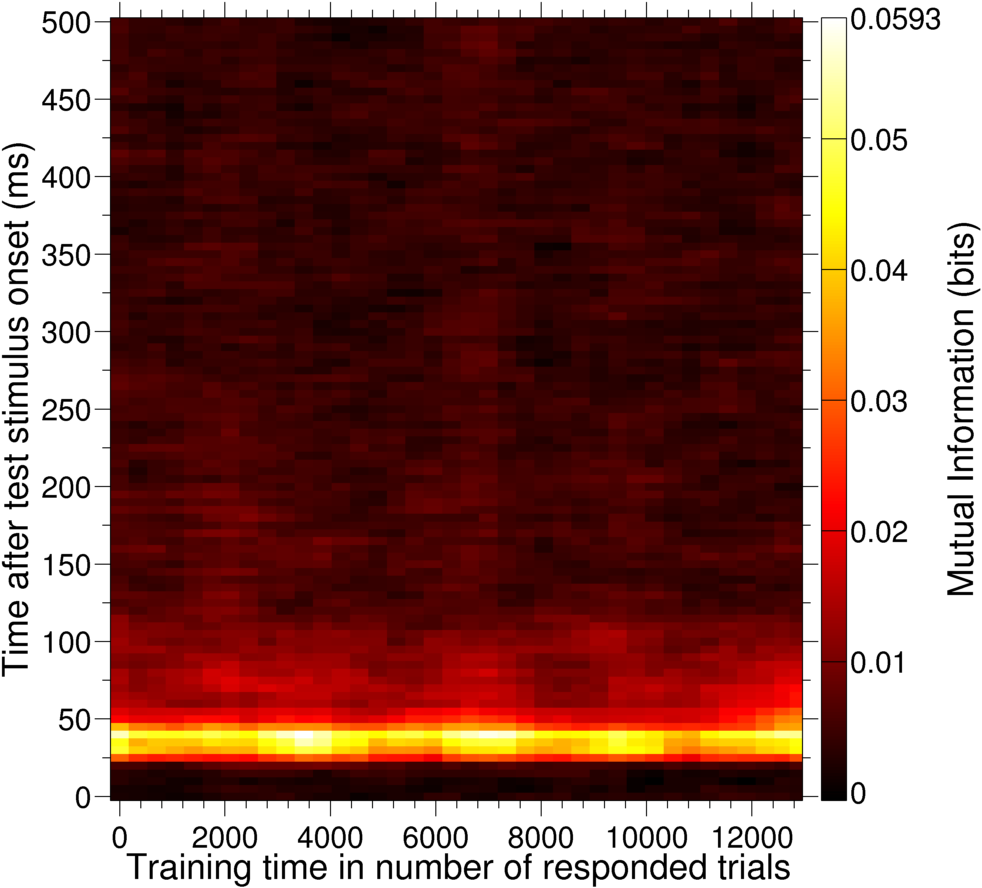
\includegraphics[scale=.25]{%
% figs/info/I_trialwise_blanco_v1_chmean23_s343-354,355.1,355.2,356-359_tp4_1bins_of_20ms_dr_pt_oc0_test_tc5-5-20,22-3-28,32,35-5-50,60,90_nt1400_ts350_rmvet1_rmvms0_pcolorhot_20120815T234452.png}
%         \caption{}
%         \label{fig:b1-1x20tp4ma}
%     \end{subfigure}
%     ~~
%     \begin{subfigure}[b]{0.5\linewidth}
%         \centering
%         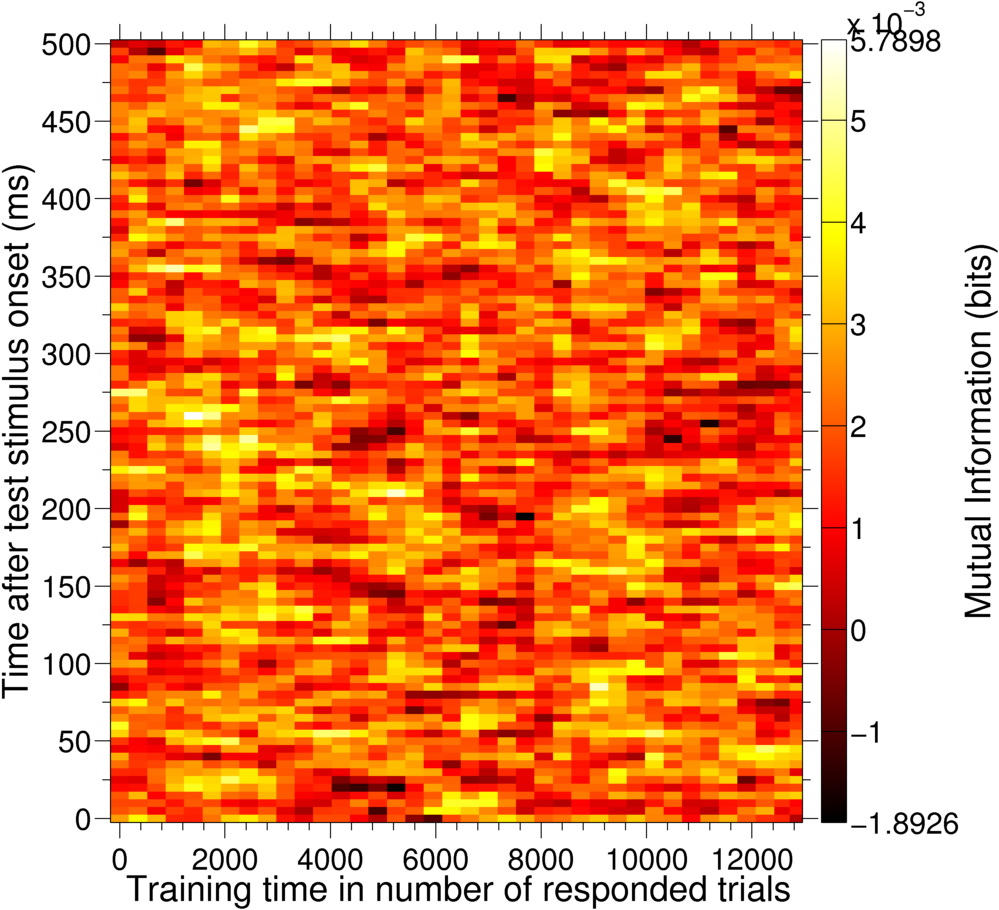
\includegraphics[scale=.25]{%
% figs/info/I_trialwise_blanco_v1_chmean23_s343-354,355.1,355.2,356-359_tp1_1bins_of_20ms_dr_pt_oc0_test_tc5-5-20,22-3-28,32,35-5-50,60,90_nt1400_ts350_rmvet1_rmvms0_pcolorhot_20120815T234326.png}
%         \caption{}
%         \label{fig:b1-1x20tp1ma}
%     \end{subfigure}
%     \\
    \begin{subfigure}[b]{0.5\linewidth}
        \centering
        \caption{}
        \label{fig:b1-1x20tp4}
        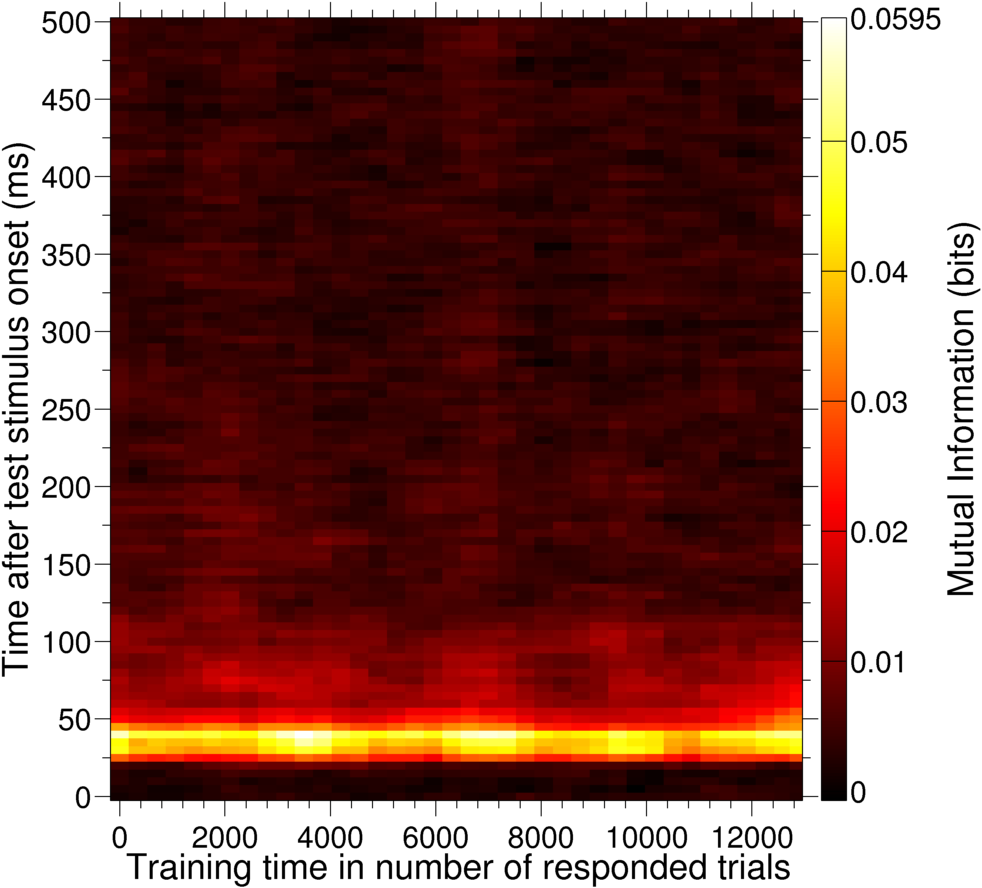
\includegraphics[scale=.25]{%
figs/info/I_trialwise_blanco_v1_chmean23_s343-354,355.1,355.2,356-359_tp4_1bins_of_20ms_dr_pt_oc0_test_tc5-5-20,22-3-28,32,35-5-50,60,90_nt1400_ts350_rmvet1_rmvms1_pcolorhot_20120815T234741.png}
    \end{subfigure}
    ~~
    \begin{subfigure}[b]{0.5\linewidth}
        \centering
        \caption{}
        \label{fig:b1-1x20tp1}
        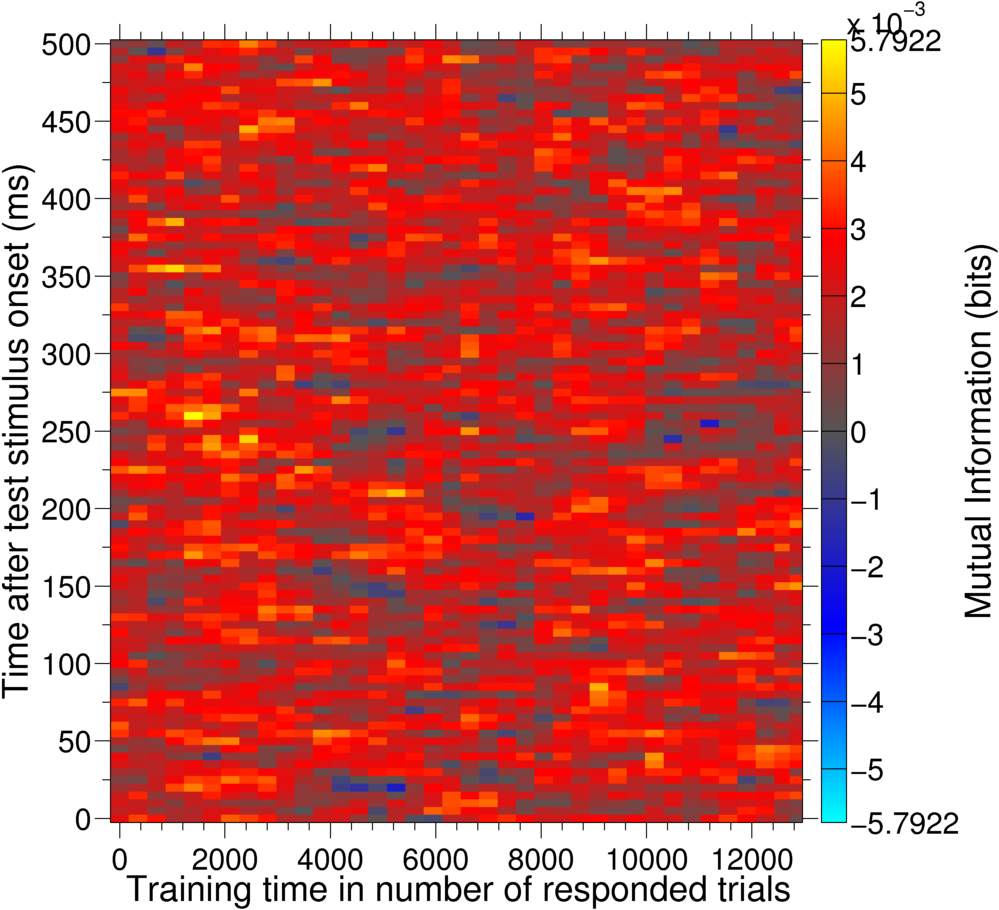
\includegraphics[scale=.25]{%
figs/info/I_trialwise_blanco_v1_chmean23_s343-354,355.1,355.2,356-359_tp1_1bins_of_20ms_dr_pt_oc0_test_tc5-5-20,22-3-28,32,35-5-50,60,90_nt1400_ts350_rmvet1_rmvms1_pcolorbp_20120816T175451.png}
    \end{subfigure}
    \\
    \begin{subfigure}[b]{0.5\linewidth}
        \centering
        \caption{}
        \label{fig:b1-5x4tp4}
        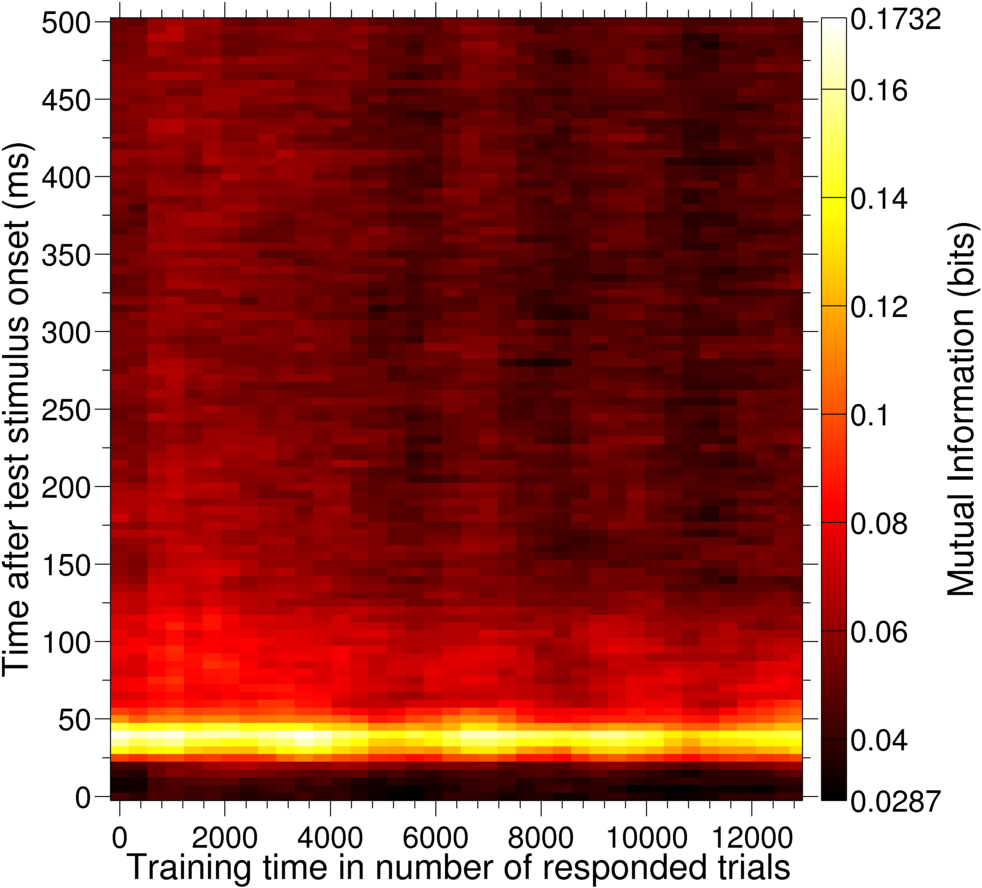
\includegraphics[scale=.25]{%
figs/info/I_trialwise_blanco_v1_chmean23_s343-354,355.1,355.2,356-359_tp4_5bins_of_4ms_dr_pt_oc0_test_tc5-5-20,22-3-28,32,35-5-50,60,90_nt1400_ts350_rmvet1_rmvms1_pcolorhot_20120815T234513.png}
    \end{subfigure}
    ~~
    \begin{subfigure}[b]{0.5\linewidth}
        \centering
        \caption{}
        \label{fig:b1-5x4tp1}
        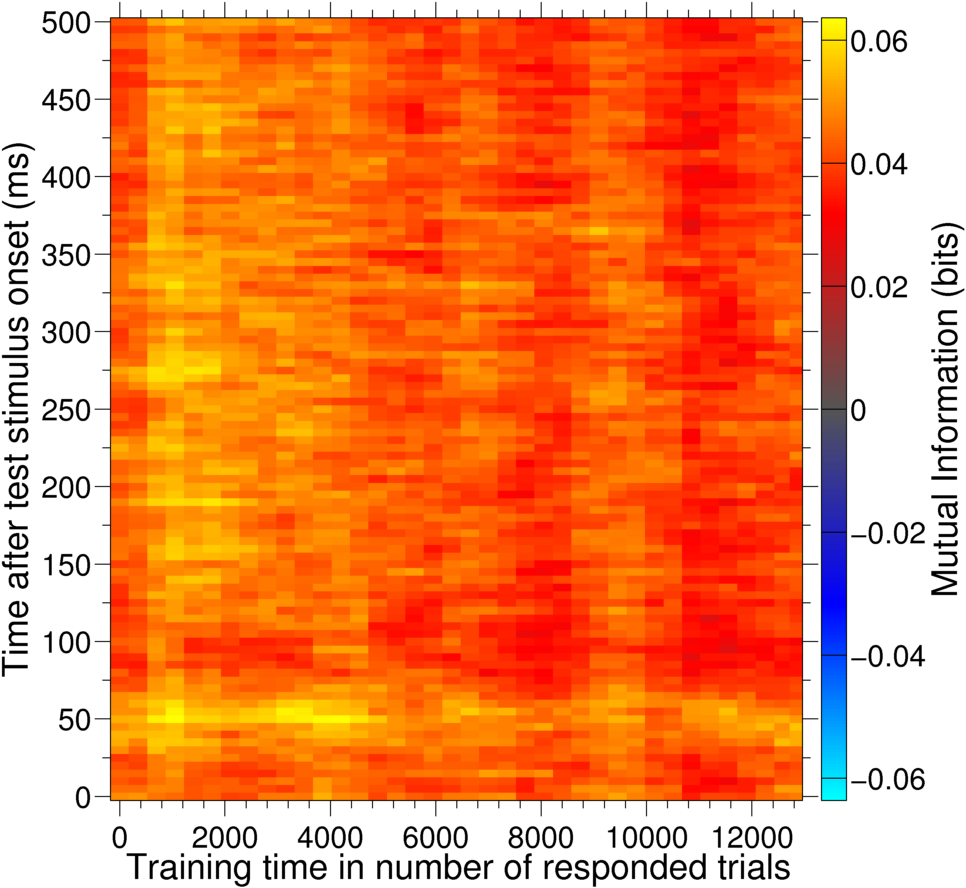
\includegraphics[scale=.25]{%
figs/info/I_trialwise_blanco_v1_chmean23_s343-354,355.1,355.2,356-359_tp1_5bins_of_4ms_dr_pt_oc0_test_tc5-5-20,22-3-28,32,35-5-50,60,90_nt1400_ts350_rmvet1_rmvms1_pcolorbp_20120816T175423.png}
    \end{subfigure}
    \caption{\ac{M1} \ac{V1}: Mutual information between the test stimulus and \SI{20}{ms} of spiking activity, averaged across 23 channels.
The \ac{PT} bias correction method was used in all estimates of the information, and the modification to the spiking data to remove the artifact as described in Sec.~\ref{sec:ma} was performed.
The neural code used in \ref{fig:b1-1x20tp4}, \ref{fig:b1-1x20tp1} is a spike count code, whilst in \ref{fig:b1-5x4tp4} and \ref{fig:b1-5x4tp1} it is a spike timing code where the \SI{20}{ms} window was subdivided into 5 bins each of \SI{4}{ms}.
In \ref{fig:b1-1x20tp4} and \ref{fig:b1-5x4tp4} the spike-train is taken from the test presentation part of the trial;
for \ref{fig:b1-1x20tp1} and \ref{fig:b1-5x4tp1} the spike-train is taken from spontaneous pre-stimulus activity.
The data is sampled in intervals of \SI{350}{trials} in the $x$-direction and \SI{5}{ms} in the $y$-direction, so there is significant correlation between any pair of pixels in the image with less than 4 pixels between them in either cartesian direction.
% In \ref{fig:b1-1x20tp4ma}, \ref{fig:b1-1x20tp4}, and \ref{fig:b1-5x4tp4}, the spike-train is taken from the test presentation part of the trial;
% for \ref{fig:b1-1x20tp1ma}, \ref{fig:b1-1x20tp1}, and \ref{fig:b1-5x4tp1}, the spike-train is taken from spontaneous pre-stimulus activity.
% In \ref{fig:b1-1x20tp4ma} and \ref{fig:b1-1x20tp1ma} no attempt was made to remove the monitor artifact from the raw data, whilst in the rest of the panels the data was modified to counter this as described in \ref{sec:ma}.
% \ref{fig:b1-1x20tp4ma}
% \ref{fig:b1-1x20tp1ma}
% \ref{fig:b1-1x20tp4}
% \ref{fig:b1-1x20tp1}
% \ref{fig:b1-5x4tp4}
% \ref{fig:b1-5x4tp1}
}
    \label{fig:b1-trialwise}
\end{figure}


% figs/info/I_trialwise_jack_v1_chmean25_s51-72_tp4_1bins_of_20ms_dr_pt_oc0_test_tc5-5-20,22-3-28,32,35-5-50,60,90_nt1400_ts350_rmvet1_rmvms0_pcolorhot_20120815T234410.png
% figs/info/I_trialwise_jack_v1_chmean25_s51-72_tp1_1bins_of_20ms_dr_pt_oc0_test_tc5-5-20,22-3-28,32,35-5-50,60,90_nt1400_ts350_rmvet1_rmvms0_pcolorhot_20120815T234245.png
% figs/info/I_trialwise_jack_v1_chmean25_s51-72_tp4_1bins_of_20ms_dr_pt_oc0_test_tc5-5-20,22-3-28,32,35-5-50,60,90_nt1400_ts350_rmvet1_rmvms1_pcolorhot_20120815T234701.png
% figs/info/I_trialwise_jack_v1_chmean25_s51-72_tp1_1bins_of_20ms_dr_pt_oc0_test_tc5-5-20,22-3-28,32,35-5-50,60,90_nt1400_ts350_rmvet1_rmvms1_pcolorbp_20120816T175411.png
% figs/info/I_trialwise_jack_v1_chmean25_s51-72_tp4_5bins_of_4ms_dr_pt_oc0_test_tc5-5-20,22-3-28,32,35-5-50,60,90_nt1400_ts350_rmvet1_rmvms1_pcolorhot_20120815T234434.png
% figs/info/I_trialwise_jack_v1_chmean25_s51-72_tp1_5bins_of_4ms_dr_pt_oc0_test_tc5-5-20,22-3-28,32,35-5-50,60,90_nt1400_ts350_rmvet1_rmvms1_pcolorbp_20120816T175343.png

\begin{figure}[htbp]
%     \begin{subfigure}[b]{0.5\linewidth}
%         \centering
%         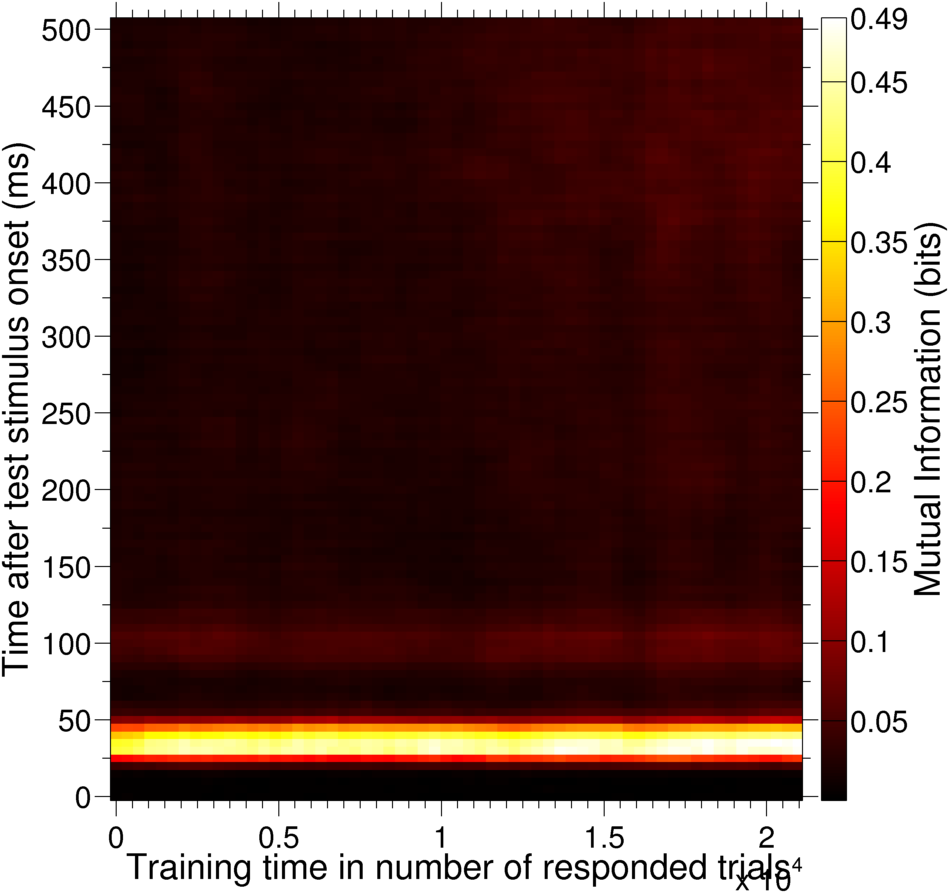
\includegraphics[scale=.25]{%
% figs/info/I_trialwise_jack_v1_chmean25_s51-72_tp4_1bins_of_20ms_dr_pt_oc0_test_tc5-5-20,22-3-28,32,35-5-50,60,90_nt1400_ts350_rmvet1_rmvms0_pcolorhot_20120815T234410.png}
%         \caption{}
%         \label{fig:j1-1x20tp4ma}
%     \end{subfigure}
%     ~~
%     \begin{subfigure}[b]{0.5\linewidth}
%         \centering
%         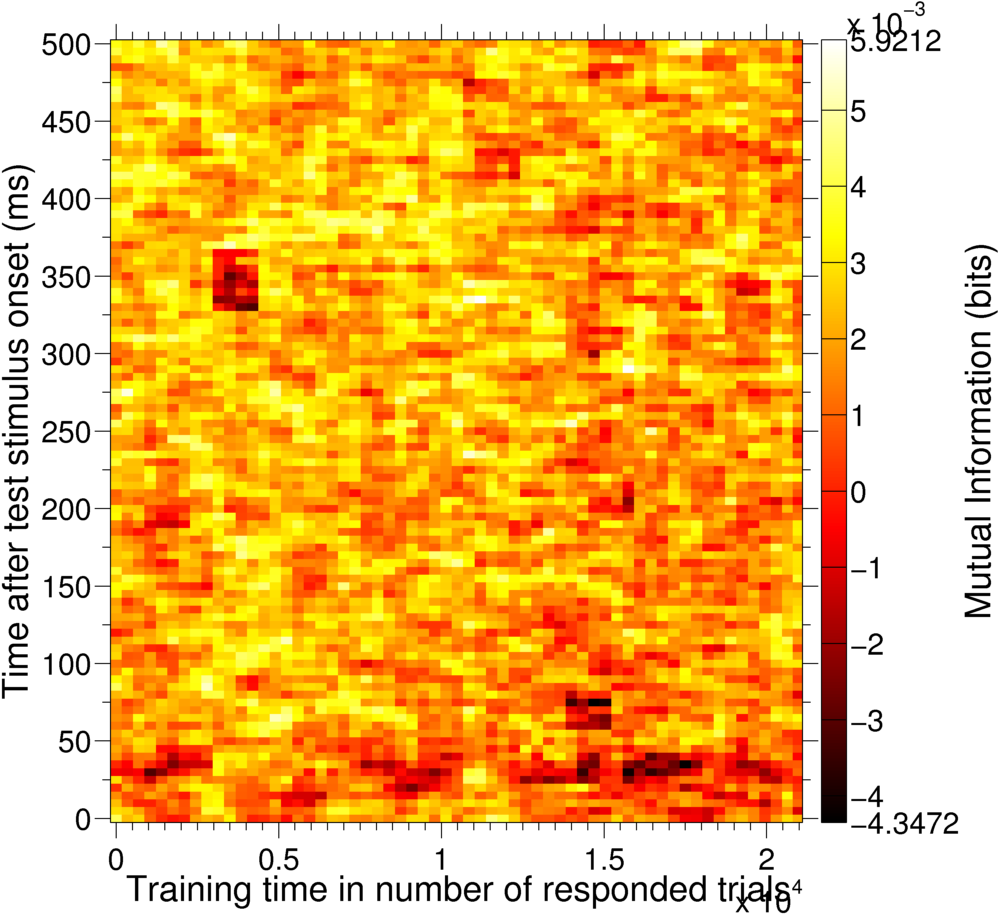
\includegraphics[scale=.25]{%
% figs/info/I_trialwise_jack_v1_chmean25_s51-72_tp1_1bins_of_20ms_dr_pt_oc0_test_tc5-5-20,22-3-28,32,35-5-50,60,90_nt1400_ts350_rmvet1_rmvms0_pcolorhot_20120815T234245.png}
%         \caption{}
%         \label{fig:j1-1x20tp1ma}
%     \end{subfigure}
%     \\
    \begin{subfigure}[b]{0.5\linewidth}
        \centering
        \caption{}
        \label{fig:j1-1x20tp4}
        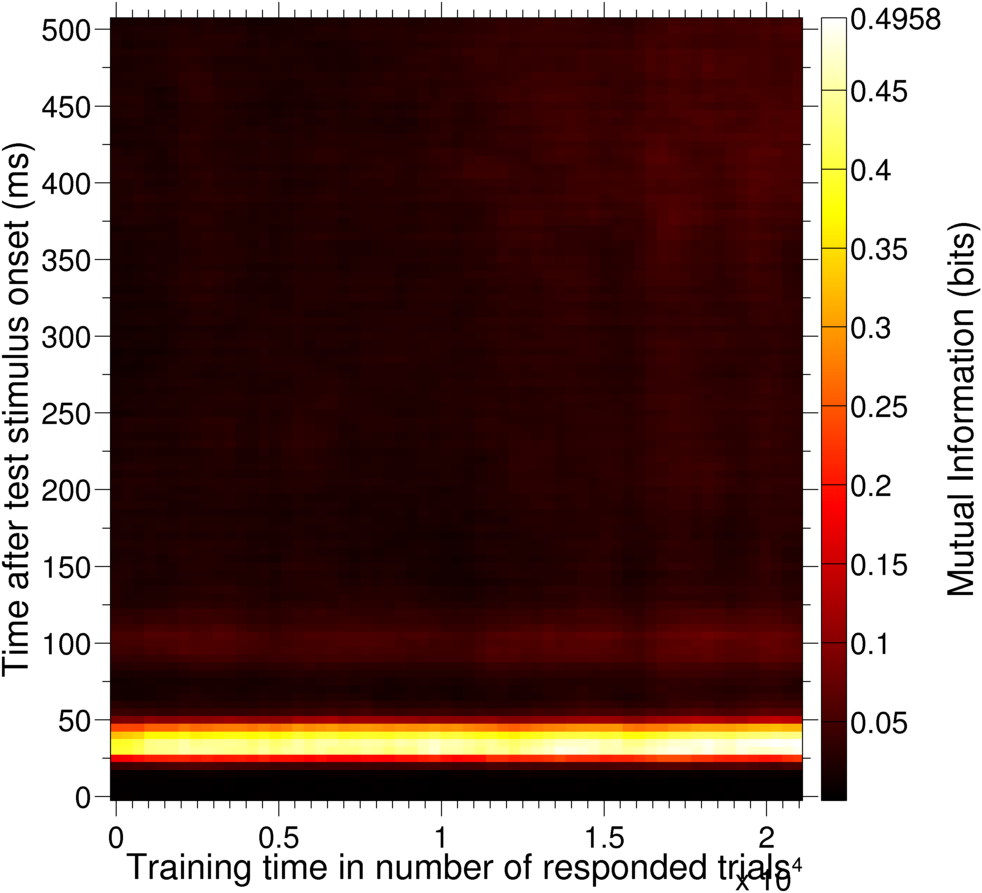
\includegraphics[scale=.25]{%
figs/info/I_trialwise_jack_v1_chmean25_s51-72_tp4_1bins_of_20ms_dr_pt_oc0_test_tc5-5-20,22-3-28,32,35-5-50,60,90_nt1400_ts350_rmvet1_rmvms1_pcolorhot_20120815T234701.png}
    \end{subfigure}
    ~~
    \begin{subfigure}[b]{0.5\linewidth}
        \centering
        \caption{}
        \label{fig:j1-1x20tp1}
        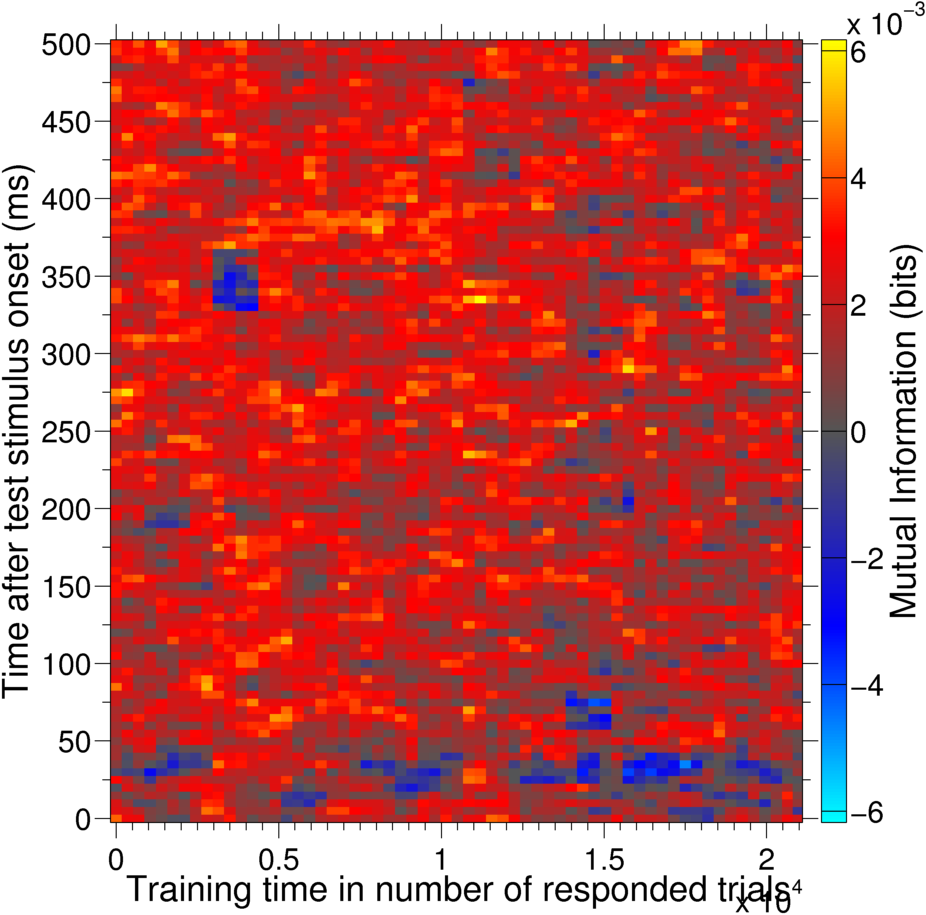
\includegraphics[scale=.25]{%
figs/info/I_trialwise_jack_v1_chmean25_s51-72_tp1_1bins_of_20ms_dr_pt_oc0_test_tc5-5-20,22-3-28,32,35-5-50,60,90_nt1400_ts350_rmvet1_rmvms1_pcolorbp_20120816T175411.png}
    \end{subfigure}
    \\
    \begin{subfigure}[b]{0.5\linewidth}
        \centering
        \caption{}
        \label{fig:j1-5x4tp4}
        \includegraphics[scale=.25]{%
figs/info/I_trialwise_jack_v1_chmean25_s51-72_tp4_5bins_of_4ms_dr_pt_oc0_test_tc5-5-20,22-3-28,32,35-5-50,60,90_nt1400_ts350_rmvet1_rmvms1_pcolorhot_20120815T234434.png}
    \end{subfigure}
    ~~
    \begin{subfigure}[b]{0.5\linewidth}
        \centering
        \caption{}
        \label{fig:j1-5x4tp1}
        \includegraphics[scale=.25]{%
figs/info/I_trialwise_jack_v1_chmean25_s51-72_tp1_5bins_of_4ms_dr_pt_oc0_test_tc5-5-20,22-3-28,32,35-5-50,60,90_nt1400_ts350_rmvet1_rmvms1_pcolorbp_20120816T175343.png}
    \end{subfigure}
    \caption{\ac{M2} \ac{V1}: Mutual information between the test stimulus and \SI{20}{ms} of spiking activity, averaged across 25 channels.
The \ac{PT} bias correction method was used in all estimates of the information.
Panels \ref{fig:j1-1x20tp4}--\ref{fig:j1-5x4tp1} are the same as for Fig.~\ref{fig:b1-trialwise}.
% The neural code used in \ref{fig:j1-1x20tp4ma}--\ref{fig:j1-1x20tp1} is a spike count code, whilst in \ref{fig:j1-5x4tp4}, \ref{fig:j1-5x4tp1} it is a spike timing code where the \SI{20}{ms} window was subdivided into 5 bins each of \SI{4}{ms}.
% In \ref{fig:j1-1x20tp4ma}, \ref{fig:j1-1x20tp4}, and \ref{fig:j1-5x4tp4}, the spike-train is taken from the test presentation part of the trial;
% for \ref{fig:j1-1x20tp1ma}, \ref{fig:j1-1x20tp1}, and \ref{fig:j1-5x4tp1}, the spike-train is taken from spontaneous pre-stimulus activity.
% In \ref{fig:j1-1x20tp4ma} and \ref{fig:j1-1x20tp1ma} no attempt was made to remove the monitor artifact from the raw data, whilst in the rest of the panels the data was modified to counter this as described in \ref{sec:ma}.
% \ref{fig:j1-1x20tp4ma}
% \ref{fig:j1-1x20tp1ma}
% \ref{fig:j1-1x20tp4}
% \ref{fig:j1-1x20tp1}
% \ref{fig:j1-5x4tp4}
% \ref{fig:j1-5x4tp1}
}
    \label{fig:j1-trialwise}
\end{figure}

% figs/info/I_trialwise_blanco_v4_chmean31_s307,308,311,313,314,317,318,320,321,329-341_tp4_1bins_of_20ms_dr_pt_oc0_test_tc10-5-25,27-29,31-33,35,40-10-60_nt1400_ts350_rmvet1_rmvms0_pcolorhot_20120815T234508.png
% figs/info/I_trialwise_blanco_v4_chmean31_s307,308,311,313,314,317,318,320,321,329-341_tp1_1bins_of_20ms_dr_pt_oc0_test_tc10-5-25,27-29,31-33,35,40-10-60_nt1400_ts350_rmvet1_rmvms0_pcolorhot_20120815T234341.png
% figs/info/I_trialwise_blanco_v4_chmean31_s307,308,311,313,314,317,318,320,321,329-341_tp4_1bins_of_20ms_dr_pt_oc0_test_tc10-5-25,27-29,31-33,35,40-10-60_nt1400_ts350_rmvet1_rmvms1_pcolorhot_20120815T234756.png
% figs/info/I_trialwise_blanco_v4_chmean31_s307,308,311,313,314,317,318,320,321,329-341_tp1_1bins_of_20ms_dr_pt_oc0_test_tc10-5-25,27-29,31-33,35,40-10-60_nt1400_ts350_rmvet1_rmvms1_pcolorbp_20120816T175507.png
% figs/info/I_trialwise_blanco_v4_chmean31_s307,308,311,313,314,317,318,320,321,329-341_tp4_5bins_of_4ms_dr_pt_oc0_test_tc10-5-25,27-29,31-33,35,40-10-60_nt1400_ts350_rmvet1_rmvms1_pcolorhot_20120815T234528.png
% figs/info/I_trialwise_blanco_v4_chmean31_s307,308,311,313,314,317,318,320,321,329-341_tp1_5bins_of_4ms_dr_pt_oc0_test_tc10-5-25,27-29,31-33,35,40-10-60_nt1400_ts350_rmvet1_rmvms1_pcolorbp_20120816T175438.png


% % \begin{figure}[htbp]
% % %     \begin{subfigure}[b]{0.5\linewidth}
% % %         \centering
% % %         \includegraphics[scale=.25]{%
% % % figs/info/I_trialwise_blanco_v4_chmean31_s307,308,311,313,314,317,318,320,321,329-341_tp4_1bins_of_20ms_dr_pt_oc0_test_tc10-5-25,27-29,31-33,35,40-10-60_nt1400_ts350_rmvet1_rmvms0_pcolorhot_20120815T234508.png}
% % %         \caption{}
% % %         \label{fig:b4-1x20tp4ma}
% % %     \end{subfigure}
% % %     ~~
% % %     \begin{subfigure}[b]{0.5\linewidth}
% % %         \centering
% % %         \includegraphics[scale=.25]{%
% % % figs/info/I_trialwise_blanco_v4_chmean31_s307,308,311,313,314,317,318,320,321,329-341_tp1_1bins_of_20ms_dr_pt_oc0_test_tc10-5-25,27-29,31-33,35,40-10-60_nt1400_ts350_rmvet1_rmvms0_pcolorhot_20120815T234341.png}
% % %         \caption{}
% % %         \label{fig:b4-1x20tp1ma}
% % %     \end{subfigure}
% % %     \\
% %     \begin{subfigure}[b]{0.5\linewidth}
% %         \centering
% %         \caption{}
% %         \label{fig:b4-1x20tp4}
% %         \includegraphics[scale=.25]{%
% % figs/info/I_trialwise_blanco_v4_chmean31_s307,308,311,313,314,317,318,320,321,329-341_tp4_1bins_of_20ms_dr_pt_oc0_test_tc10-5-25,27-29,31-33,35,40-10-60_nt1400_ts350_rmvet1_rmvms1_pcolorhot_20120815T234756.png}
% %     \end{subfigure}
% %     ~~
% %     \begin{subfigure}[b]{0.5\linewidth}
% %         \centering
% %         \caption{}
% %         \label{fig:b4-1x20tp1}
% %         \includegraphics[scale=.25]{%
% % figs/info/I_trialwise_blanco_v4_chmean31_s307,308,311,313,314,317,318,320,321,329-341_tp1_1bins_of_20ms_dr_pt_oc0_test_tc10-5-25,27-29,31-33,35,40-10-60_nt1400_ts350_rmvet1_rmvms1_pcolorbp_20120816T175507.png}
% %     \end{subfigure}
% %     \\
% %     \begin{subfigure}[b]{0.5\linewidth}
% %         \centering
% %         \caption{}
% %         \label{fig:b4-5x4tp4}
% %         \includegraphics[scale=.25]{%
% % figs/info/I_trialwise_blanco_v4_chmean31_s307,308,311,313,314,317,318,320,321,329-341_tp4_5bins_of_4ms_dr_pt_oc0_test_tc10-5-25,27-29,31-33,35,40-10-60_nt1400_ts350_rmvet1_rmvms1_pcolorhot_20120815T234528.png}
% %     \end{subfigure}
% %     ~~
% %     \begin{subfigure}[b]{0.5\linewidth}
% %         \centering
% %         \caption{}
% %         \label{fig:b4-5x4tp1}
% %         \includegraphics[scale=.25]{%
% % figs/info/I_trialwise_blanco_v4_chmean31_s307,308,311,313,314,317,318,320,321,329-341_tp1_5bins_of_4ms_dr_pt_oc0_test_tc10-5-25,27-29,31-33,35,40-10-60_nt1400_ts350_rmvet1_rmvms1_pcolorbp_20120816T175438.png}
% %     \end{subfigure}
% %     \caption{\ac{M1} \ac{V4}: Mutual information between the test stimulus and \SI{20}{ms} of spiking activity, averaged across 30 channels.
% % The \ac{PT} bias correction method was used in all estimates of the information.
% % Panels \ref{fig:b4-1x20tp4}--\ref{fig:b4-5x4tp1} are the same as for Fig.~\ref{fig:b1-trialwise}.
% % % The neural code used in \ref{fig:b4-1x20tp4ma}--\ref{fig:b4-1x20tp1} is a spike count code, whilst in \ref{fig:b4-5x4tp4}, \ref{fig:b4-5x4tp1} it is a spike timing code where the \SI{20}{ms} window was subdivided into 5 bins each of \SI{4}{ms}.
% % % In \ref{fig:b4-1x20tp4ma}, \ref{fig:b4-1x20tp4}, and \ref{fig:b4-5x4tp4}, the spike-train is taken from the test presentation part of the trial;
% % % for \ref{fig:b4-1x20tp1ma}, \ref{fig:b4-1x20tp1}, and \ref{fig:b4-5x4tp1}, the spike-train is taken from spontaneous pre-stimulus activity.
% % % In \ref{fig:b4-1x20tp4ma} and \ref{fig:b4-1x20tp1ma} no attempt was made to remove the monitor artifact from the raw data, whilst in the rest of the panels the data was modified to counter this as described in \ref{sec:ma}.
% % % \ref{fig:b4-1x20tp4ma}
% % % \ref{fig:b4-1x20tp1ma}
% % % \ref{fig:b4-1x20tp4}
% % % \ref{fig:b4-1x20tp1}
% % % \ref{fig:b4-5x4tp4}
% % % \ref{fig:b4-5x4tp1}
% % }
% %     \label{fig:b4-trialwise}
% % \end{figure}



% figs/info/I_trialwise_jack_v4_chmean20_s24-49_tp4_1bins_of_20ms_dr_pt_oc0_test_tc10-5-25,27-29,31-33,35,40-10-60_nt1400_ts350_rmvet1_rmvms0_pcolorhot_20120815T234433.png
% figs/info/I_trialwise_jack_v4_chmean20_s24-49_tp1_1bins_of_20ms_dr_pt_oc0_test_tc10-5-25,27-29,31-33,35,40-10-60_nt1400_ts350_rmvet1_rmvms1_pcolorbp_20120816T175433.png
% figs/info/I_trialwise_jack_v4_chmean20_s24-49_tp4_1bins_of_20ms_dr_pt_oc0_test_tc10-5-25,27-29,31-33,35,40-10-60_nt1400_ts350_rmvet1_rmvms1_pcolorhot_20120815T234723.png
% figs/info/I_trialwise_jack_v4_chmean20_s24-49_tp1_1bins_of_20ms_dr_pt_oc0_test_tc10-5-25,27-29,31-33,35,40-10-60_nt1400_ts350_rmvet1_rmvms1_pcolorhot_20120815T234559.png
% figs/info/I_trialwise_jack_v4_chmean20_s24-49_tp4_5bins_of_4ms_dr_pt_oc0_test_tc10-5-25,27-29,31-33,35,40-10-60_nt1400_ts350_rmvet1_rmvms1_pcolorhot_20120815T234455.png
% figs/info/I_trialwise_jack_v4_chmean20_s24-49_tp1_5bins_of_4ms_dr_pt_oc0_test_tc10-5-25,27-29,31-33,35,40-10-60_nt1400_ts350_rmvet1_rmvms1_pcolorbp_20120816T175404.png

\begin{figure}[htbp]
%     \begin{subfigure}[b]{0.5\linewidth}
%         \centering
%         \includegraphics[scale=.25]{%
% figs/info/I_trialwise_jack_v4_chmean20_s24-49_tp4_1bins_of_20ms_dr_pt_oc0_test_tc10-5-25,27-29,31-33,35,40-10-60_nt1400_ts350_rmvet1_rmvms0_pcolorhot_20120815T234433.png}
%         \caption{}
%         \label{fig:j4-1x20tp4ma}
%     \end{subfigure}
%     ~~
%     \begin{subfigure}[b]{0.5\linewidth}
%         \centering
%         \includegraphics[scale=.25]{%
% figs/info/I_trialwise_jack_v4_chmean20_s24-49_tp1_1bins_of_20ms_dr_pt_oc0_test_tc10-5-25,27-29,31-33,35,40-10-60_nt1400_ts350_rmvet1_rmvms0_pcolorhot_20120815T234307.png}
%         \caption{}
%         \label{fig:j4-1x20tp1ma}
%     \end{subfigure}
%     \\
    \begin{subfigure}[b]{0.5\linewidth}
        \centering
        \caption{}
        \label{fig:j4-1x20tp4}
        \includegraphics[scale=.25]{%
figs/info/I_trialwise_jack_v4_chmean20_s24-49_tp4_1bins_of_20ms_dr_pt_oc0_test_tc10-5-25,27-29,31-33,35,40-10-60_nt1400_ts350_rmvet1_rmvms1_pcolorhot_20120815T234723.png}
    \end{subfigure}
    ~~
    \begin{subfigure}[b]{0.5\linewidth}
        \centering
        \caption{}
        \label{fig:j4-1x20tp1}
        \includegraphics[scale=.25]{%
figs/info/I_trialwise_jack_v4_chmean20_s24-49_tp1_1bins_of_20ms_dr_pt_oc0_test_tc10-5-25,27-29,31-33,35,40-10-60_nt1400_ts350_rmvet1_rmvms1_pcolorbp_20120816T175433.png}
    \end{subfigure}
    \\
    \begin{subfigure}[b]{0.5\linewidth}
        \centering
        \caption{}
        \label{fig:j4-5x4tp4}
        \includegraphics[scale=.25]{%
figs/info/I_trialwise_jack_v4_chmean20_s24-49_tp4_5bins_of_4ms_dr_pt_oc0_test_tc10-5-25,27-29,31-33,35,40-10-60_nt1400_ts350_rmvet1_rmvms1_pcolorhot_20120815T234455.png}
    \end{subfigure}
    ~~
    \begin{subfigure}[b]{0.5\linewidth}
        \centering
        \caption{}
        \label{fig:j4-5x4tp1}
        \includegraphics[scale=.25]{%
figs/info/I_trialwise_jack_v4_chmean20_s24-49_tp1_5bins_of_4ms_dr_pt_oc0_test_tc10-5-25,27-29,31-33,35,40-10-60_nt1400_ts350_rmvet1_rmvms1_pcolorbp_20120816T175404.png}
    \end{subfigure}
    \caption{\ac{M2} \ac{V4}: Mutual information between the test stimulus and \SI{20}{ms} of spiking activity, averaged across 20 channels.
The \ac{PT} bias correction method was used in all estimates of the information.
Panels \ref{fig:j4-1x20tp4}--\ref{fig:j4-5x4tp1} are the same as for Fig.~\ref{fig:b1-trialwise}.
% The neural code used in \ref{fig:j4-1x20tp4ma}--\ref{fig:j4-1x20tp1} is a spike count code, whilst in \ref{fig:j4-5x4tp4}, \ref{fig:j4-5x4tp1} it is a spike timing code where the \SI{20}{ms} window was subdivided into 5 bins each of \SI{4}{ms}.
% In \ref{fig:j4-1x20tp4ma}, \ref{fig:j4-1x20tp4}, and \ref{fig:j4-5x4tp4}, the spike-train is taken from the test presentation part of the trial;
% for \ref{fig:j4-1x20tp1ma}, \ref{fig:j4-1x20tp1}, and \ref{fig:j4-5x4tp1}, the spike-train is taken from spontaneous pre-stimulus activity.
% In \ref{fig:j4-1x20tp4ma} and \ref{fig:j4-1x20tp1ma} no attempt was made to remove the monitor artifact from the raw data, whilst in the rest of the panels the data was modified to counter this as described in \ref{sec:ma}.
% \ref{fig:j4-1x20tp4ma}
% \ref{fig:j4-1x20tp1ma}
% \ref{fig:j4-1x20tp4}
% \ref{fig:j4-1x20tp1}
% \ref{fig:j4-5x4tp4}
% \ref{fig:j4-5x4tp1}
}
    \label{fig:j4-trialwise}
\end{figure}

% 20, 30 and \SI{40}{ms} all tried.
% Mutual information increases as the duration increases as one would expect, but there is no other significant difference.
% Consequently only 20ms is shown in this section.

% More information with only correct trials used, but this could be due to differences in $P(S)$.

Turning our attention to the \ac{V4} results in Figs.~\ref{fig:b4-trialwise} and \ref{fig:j4-trialwise}, we can see the effect of the transient is present in \ac{M1}'s data (at the later start time of \SI{75}{ms}), but not in \ac{M2}'s.
This is surprising because, looking at the rasters, in both animals there are some channels which exhibit a transient response and some which do not.

Similar to \ac{V1}, it seems as if there is four times as much information in the timebinned code compared with the count code.
However, there is much more information measured for the spontaneous activity data again.
This is not reduced by increasing the number of trials either.

For the spike count code in \ac{M2}, the spontaneous information is nearly distributed around 0, suggesting the bias has been all but removed and the data is of very high quality.
For this animal, we can see a distinct increase in the information content with time, for both the spike count and timing codes.
Simultaneously, there is a movement of the peak information to earlier times closer to the stimulus onset.

In \ac{M1}, there is a small increase in the information content with time which may or may not significant.
However, it is reassuring to see that this is not due to an improvement in the data with time, as the trend in the spontaneous activity information bias (Fig.~\ref{fig:j4-5x4tp1}) is a decrease with time.


%------------------------------------------------------------------------------
\subsection{Information in fine vs. coarse distinctions}

The difference between information about fine differences in contrast can be studied by only considering trials where the contrast presented is one of the middle 6 contrasts:
\SIlist{22;25;28;32;35;40}{\percent} for \ac{V1} and
\SIlist{27;28;29;31;32;33}{\percent} for \ac{V4}.
To keep the dimensionality of the stimulus the same, this has been compared to the information across some more separated contrasts:
\SIlist{5;15;22;40;50;90}{\percent} for \ac{V1} and
\SIlist{10;15;20;40;50;60}{\percent} for \ac{V4}.
For \ac{V4}, the group of coarsely differentiated contrasts is the outer most six contrasts, but for \ac{V1} the coarsely differentiated contrasts are alternate


\subsubsection{Results}

Comparing Figs.~\ref{fig:b1-1x20cc} and \ref{fig:j1-1x20cc} where the outer 6 contrasts are included with Figs.~\ref{fig:b1-1x20tp4} and \ref{fig:b1-1x20tp4} where all contrasts are included, it seems as if the amount of information has increased, which should not be possible.
However, the difference will be due to the difference in trials contained in each of the analyses.
In each case, an average of 100 trials per stimulus is used, but since the easier test conditions are presented less frequently, they are under-represented in Figs.~\ref{fig:b1-1x20tp4} and \ref{fig:b1-1x20tp4} (about 75 trials per stimulus).
Obviously these are more discriminable, so the under-representation comparably reduces the information.

Looking at \ac{V1} (Fig.~\ref{fig:v1-fvc}), we observe there is much more information for \ac{M2} than \ac{M1}, as we found before.
The quality of the data seems to have severely hampered the analysis for \ac{M1}, destroying the the fine differences in the data needed to evaluate the information contained about fine contrast differences (Fig.~\ref{fig:b1-1x20fc}).

Unsurprisingly, there is more information when considering the coarsely distinct contrasts than the finer differences, as the neural activity is bound to be more discriminable for these.
For \ac{M2}, there is a small upward trend again for both coarse and fine contrast differences, which may or may not be genuine.

% figs/info/I_trialwise_blanco_v1_chmean23_s343-354,355.1,355.2,356-359_tp4_1bins_of_20ms_dr_pt_oc0_test_tc5,15,22,40,50,90_nt600_ts150_rmvet1_rmvms1_pcolorhot_20120816T011936.png
% figs/info/I_trialwise_blanco_v1_chmean23_s343-354,355.1,355.2,356-359_tp4_1bins_of_20ms_dr_pt_oc0_test_tc22-3-28,32,35,40_nt600_ts150_rmvet1_rmvms1_pcolorhot_20120816T011920.png
% figs/info/I_trialwise_jack_v1_chmean25_s51-72_tp4_1bins_of_20ms_dr_pt_oc0_test_tc5,15,22,40,50,90_nt600_ts150_rmvet1_rmvms1_pcolorhot_20120816T011822.png
% figs/info/I_trialwise_jack_v1_chmean25_s51-72_tp4_1bins_of_20ms_dr_pt_oc0_test_tc22-3-28,32,35,40_nt600_ts150_rmvet1_rmvms1_pcolorhot_20120816T011800.png

\begin{figure}[htbp]
    \begin{subfigure}[b]{0.5\linewidth}
        \centering
        \caption{}
        \label{fig:b1-1x20cc}
        \includegraphics[scale=.25]{%
figs/info/I_trialwise_blanco_v1_chmean23_s343-354,355.1,355.2,356-359_tp4_1bins_of_20ms_dr_pt_oc0_test_tc5,15,22,40,50,90_nt600_ts150_rmvet1_rmvms1_pcolorhot_20120816T011936.png}
    \end{subfigure}
    ~~
    \begin{subfigure}[b]{0.5\linewidth}
        \centering
        \caption{}
        \label{fig:j1-1x20cc}
        \includegraphics[scale=.25]{%
figs/info/I_trialwise_jack_v1_chmean25_s51-72_tp4_1bins_of_20ms_dr_pt_oc0_test_tc5,15,22,40,50,90_nt600_ts150_rmvet1_rmvms1_pcolorhot_20120816T011822.png}
    \end{subfigure}
    \\
    \begin{subfigure}[b]{0.5\linewidth}
        \centering
        \caption{}
        \label{fig:b1-1x20fc}
        \includegraphics[scale=.25]{%
figs/info/I_trialwise_blanco_v1_chmean23_s343-354,355.1,355.2,356-359_tp4_1bins_of_20ms_dr_pt_oc0_test_tc22-3-28,32,35,40_nt600_ts150_rmvet1_rmvms1_pcolorhot_20120816T011920.png}
    \end{subfigure}
    ~~
    \begin{subfigure}[b]{0.5\linewidth}
        \centering
        \caption{}
        \label{fig:j1-1x20fc}
        \includegraphics[scale=.25]{%
figs/info/I_trialwise_jack_v1_chmean25_s51-72_tp4_1bins_of_20ms_dr_pt_oc0_test_tc22-3-28,32,35,40_nt600_ts150_rmvet1_rmvms1_pcolorhot_20120816T011800.png}
    \end{subfigure}
    \caption{\ac{V1}: Fine vs. coarse contrast differences.
% Mutual information between the test stimulus and \SI{20}{ms} of spiking activity.
% The \ac{PT} bias correction method was used in all estimates of the information.
In the top panels, the six contrasts included are \{5, 15, 22, 40, 50, 90\}\%; bottom panels \{22, 25, 28, 32, 35, 40\}\%.
An average of 100 trials per stimulus is used in each of these.
Left panels are for \ac{M1}, right are \ac{M2}.
In each case, mutual information between the six test stimuli and \SI{20}{ms} of spiking activity was measured using a spike count code, and bias corrected using the \ac{PT} method.
% Panels \ref{fig:b1-1x20cc} and \ref{fig:b1-1x20fc} are for \ac{M1}, \ref{fig:b1-1x20cc} and \ref{fig:b1-1x20fc} for \ac{M2}.
}
    \label{fig:v1-fvc}
\end{figure}


% figs/info/I_trialwise_blanco_v4_chmean31_s307,308,311,313,314,317,318,320,321,329-341_tp4_1bins_of_20ms_dr_pt_oc0_test_tc10-5-20,40-10-60_nt600_ts150_rmvet1_rmvms1_pcolorhot_20120816T012120.png
% figs/info/I_trialwise_blanco_v4_chmean31_s307,308,311,313,314,317,318,320,321,329-341_tp4_1bins_of_20ms_dr_pt_oc0_test_tc27-29,31-33_nt600_ts150_rmvet1_rmvms1_pcolorhot_20120816T011952.png
% figs/info/I_trialwise_jack_v4_chmean20_s24-49_tp4_1bins_of_20ms_dr_pt_oc0_test_tc10-5-20,40-10-60_nt600_ts150_rmvet1_rmvms1_pcolorhot_20120816T011902.png
% figs/info/I_trialwise_jack_v4_chmean20_s24-49_tp4_1bins_of_20ms_dr_pt_oc0_test_tc27-29,31-33_nt600_ts150_rmvet1_rmvms1_pcolorhot_20120816T011843.png

\begin{figure}[htbp]
    \begin{subfigure}[b]{0.5\linewidth}
        \centering
        \caption{}
        \label{fig:b4-1x20cc}
        \includegraphics[scale=.25]{%
figs/info/I_trialwise_blanco_v4_chmean31_s307,308,311,313,314,317,318,320,321,329-341_tp4_1bins_of_20ms_dr_pt_oc0_test_tc10-5-20,40-10-60_nt600_ts150_rmvet1_rmvms1_pcolorhot_20120816T012120.png}
    \end{subfigure}
    ~~
    \begin{subfigure}[b]{0.5\linewidth}
        \centering
        \caption{}
        \label{fig:j4-1x20cc}
        \includegraphics[scale=.25]{%
figs/info/I_trialwise_jack_v4_chmean20_s24-49_tp4_1bins_of_20ms_dr_pt_oc0_test_tc10-5-20,40-10-60_nt600_ts150_rmvet1_rmvms1_pcolorhot_20120816T011902.png}
    \end{subfigure}
    \\
    \begin{subfigure}[b]{0.5\linewidth}
        \centering
        \caption{}
        \label{fig:b4-1x20fc}
        \includegraphics[scale=.25]{%
figs/info/I_trialwise_blanco_v4_chmean31_s307,308,311,313,314,317,318,320,321,329-341_tp4_1bins_of_20ms_dr_pt_oc0_test_tc27-29,31-33_nt600_ts150_rmvet1_rmvms1_pcolorhot_20120816T011952.png}
    \end{subfigure}
    ~~
    \begin{subfigure}[b]{0.5\linewidth}
        \centering
        \caption{}
        \label{fig:j4-1x20fc}
        \includegraphics[scale=.25]{%
figs/info/I_trialwise_jack_v4_chmean20_s24-49_tp4_1bins_of_20ms_dr_pt_oc0_test_tc27-29,31-33_nt600_ts150_rmvet1_rmvms1_pcolorhot_20120816T011843.png}
    \end{subfigure}
    \caption{\ac{V4}: Fine vs coarse contrast differences.
% Mutual information between the test stimulus and \SI{20}{ms} of spiking activity.
% The \ac{PT} bias correction method was used in all estimates of the information.
In the top panels, the six contrasts included are \{10, 15, 20, 40, 50, 60\}\%; bottom panels \{27, 28, 29, 31, 32, 33\}\%. An average of 100 trials per stimulus is used in each of these.
Left panels are for \ac{M1}, right are \ac{M2}.
In each case, mutual information between the six test stimuli and \SI{20}{ms} of spiking activity was measured using a spike count code, and bias corrected using the \ac{PT} method.
% Panels \ref{fig:b1-1x20cc} and \ref{fig:b1-1x20fc} are for \ac{M1}, \ref{fig:b1-1x20cc} and \ref{fig:b1-1x20fc} for \ac{M2}.
}
    \label{fig:v4-fvc}
\end{figure}

For \ac{V4}, we find there is no information about fine contrast differences in either animal (Figs.~\ref{fig:b4-1x20fc} and \ref{fig:j4-1x20fc}).
The information about the coarse differences is higher than when all conditions are considered, for reasons discussed above, and these show the same trends as when we analysed all the conditions, in Figs.~\ref{fig:b4-1x20tp4} and \ref{fig:j4-1x20tp4}.


\subsubsection{Discussion}

We did not find that learning was focused on the more difficult contrasts with the fine differences between them.
If there is an increase in the information in \ac{V1}, it is not very large and occurs for all groups of contrasts to the same degree.
Curiously, for \ac{V4}, it seems that the neurons improve their discriminability for the coarsely differentiated contrasts, but not the fine differences, which is the opposite to what was anticipated.
It could be that fine stimuli differences cannot be accurately resolved using the signals from only individual neurons, and concurrent signals from a population of neurons are needed for this to be finer discrimination to be possible.


%------------------------------------------------------------------------------
\subsection{Information in spike timing code vs. spike count code}

Because the possible responses in the spike timing and count codes have different dimensionality, they have different biases \citep{Panzeri2007} and it is not possible to compare them directly.
Consequently, to investigate how much more information there is in a spike timing based code we must consider a set of responses which have the same dimensionality, but lack the timing information.

To do this, the spike-timing response codes are taken, then shuffled across the 5 bins for every individual trial.%
\footnote{The shuffling of bins was performed using the open source Shuffle.m
available from \url{http://www.mathworks.com/matlabcentral/fileexchange/27076-shuffle}.}
Since the 5 bins are now in a random order, any information contained in their order is lost.
To make ensure the estimate of the information in the spike-timing code with the timing information destroyed was reasonable, the information was measured for five different shuffles%
% \footnote{The five shuffles were performed with a random seed linked to microsecond of execution time.}
 and then the mean was taken.

The information contained in the \SI{4}{ms} level spike timing can then be found by subtracting the mean shuffled information from the unshuffled information.


\subsubsection{Results}

For \ac{M2} \ac{V1}, there seems to be some information in the millisecond-level timing of the spikes during the transient response, but not afterward this has elapsed (Fig.~\ref{fig:v1-dif}, right-hand panels).
This band due to the transient is clearly well above the variance of the sampling for the rest of the window offsets.
However, the information in the transient is only present for the coarse contrasts and not for the fine contrasts.
For the fine contrast discrimination in \ac{M2} \ac{V1}, shown in Fig.~\ref{fig:j1-fdif}, (and possibly to a lesser degree on a couple of the other figures) there is an unusual effect where there seems to be more information in the shuffled bins than the unshuffled bins.\footnote{When this is analysed for the raw data with the artifact included, this is subtly more prominently on several of the plots.}

For \ac{M1} \ac{V1}, and also \ac{M1} \ac{V4}, there seems to be an increase in the information contained in the spike timing during the transient also.
However, these results are not as clear-cut as in \ac{M2} \ac{V1}.

% figs/info/I_diff_trialwise_dur=20ms_nshuf=1_blanco_v1_chmean23_s343-354,355.1,355.2,356-359_tp4_dr_pt_oc0_test_tc5-5-20,22-3-28,32,35-5-50,60,90_nt1400_ts350_rmvet1_rmvms1_pcolorbp_20120816T010538.png
% figs/info/I_diff_trialwise_dur=20ms_nshuf=1_blanco_v1_chmean23_s343-354,355.1,355.2,356-359_tp4_dr_pt_oc0_test_tc5,15,22,40,50,90_nt600_ts150_rmvet1_rmvms1_pcolorbp_20120816T004933.png
% figs/info/I_diff_trialwise_dur=20ms_nshuf=1_blanco_v1_chmean23_s343-354,355.1,355.2,356-359_tp4_dr_pt_oc0_test_tc22-3-28,32,35,40_nt600_ts150_rmvet1_rmvms1_pcolorbp_20120816T004908.png
% 
% figs/info/I_diff_trialwise_dur=20ms_nshuf=1_jack_v1_chmean25_s51-72_tp4_dr_pt_oc0_test_tc5-5-20,22-3-28,32,35-5-50,60,90_nt1400_ts350_rmvet1_rmvms1_pcolorbp_20120816T004517.png
% figs/info/I_diff_trialwise_dur=20ms_nshuf=1_jack_v1_chmean25_s51-72_tp4_dr_pt_oc0_test_tc5,15,22,40,50,90_nt600_ts150_rmvet1_rmvms1_pcolorbp_20120816T010526.png
% figs/info/I_diff_trialwise_dur=20ms_nshuf=1_jack_v1_chmean25_s51-72_tp4_dr_pt_oc0_test_tc22-3-28,32,35,40_nt600_ts150_rmvet1_rmvms1_pcolorbp_20120816T004555.png

\begin{figure}[htbp]
    \begin{subfigure}[b]{0.5\linewidth}
        \centering
        \caption{}
        \label{fig:b1-alldif}
        \includegraphics[scale=.25]{%
figs/info/I_diff_trialwise_dur=20ms_nshuf=1_blanco_v1_chmean23_s343-354,355.1,355.2,356-359_tp4_dr_pt_oc0_test_tc5-5-20,22-3-28,32,35-5-50,60,90_nt1400_ts350_rmvet1_rmvms1_pcolorbp_20120816T010538.png}
    \end{subfigure}
    ~~
    \begin{subfigure}[b]{0.5\linewidth}
        \centering
        \caption{}
        \label{fig:j1-alldif}
        \includegraphics[scale=.25]{%
figs/info/I_diff_trialwise_dur=20ms_nshuf=1_jack_v1_chmean25_s51-72_tp4_dr_pt_oc0_test_tc5-5-20,22-3-28,32,35-5-50,60,90_nt1400_ts350_rmvet1_rmvms1_pcolorbp_20120816T004517.png}
    \end{subfigure}
    \\
    \begin{subfigure}[b]{0.5\linewidth}
        \centering
        \caption{}
        \label{fig:b1-cdif}
        \includegraphics[scale=.25]{%
figs/info/I_diff_trialwise_dur=20ms_nshuf=1_blanco_v1_chmean23_s343-354,355.1,355.2,356-359_tp4_dr_pt_oc0_test_tc5,15,22,40,50,90_nt600_ts150_rmvet1_rmvms1_pcolorbp_20120816T004933.png}
    \end{subfigure}
    ~~
    \begin{subfigure}[b]{0.5\linewidth}
        \centering
        \caption{}
        \label{fig:j1-cdif}
        \includegraphics[scale=.25]{%
figs/info/I_diff_trialwise_dur=20ms_nshuf=1_jack_v1_chmean25_s51-72_tp4_dr_pt_oc0_test_tc5,15,22,40,50,90_nt600_ts150_rmvet1_rmvms1_pcolorbp_20120816T010526.png}
    \end{subfigure}
    \\
    \begin{subfigure}[b]{0.5\linewidth}
        \centering
        \caption{}
        \label{fig:b1-fdif}
        \includegraphics[scale=.25]{%
figs/info/I_diff_trialwise_dur=20ms_nshuf=1_blanco_v1_chmean23_s343-354,355.1,355.2,356-359_tp4_dr_pt_oc0_test_tc22-3-28,32,35,40_nt600_ts150_rmvet1_rmvms1_pcolorbp_20120816T004908.png}
    \end{subfigure}
    ~~
    \begin{subfigure}[b]{0.5\linewidth}
        \centering
        \caption{}
        \label{fig:j1-fdif}
        \includegraphics[scale=.25]{%
figs/info/I_diff_trialwise_dur=20ms_nshuf=1_jack_v1_chmean25_s51-72_tp4_dr_pt_oc0_test_tc22-3-28,32,35,40_nt600_ts150_rmvet1_rmvms1_pcolorbp_20120816T004555.png}
    \end{subfigure}
    \caption{\ac{V1}: Information in millisecond level spike timing.
% Mutual information between the test stimulus and \SI{20}{ms} of spiking activity.
% The \ac{PT} bias correction method was used in all estimates of the information.
The information with time-wise shuffled bins was subtracted from information in the spike time code with a \SI{20}{ms} window subdivided into 5 bins.
Information was bias corrected using the \ac{PT} method.
Left panels: \ac{M1}; Right: \ac{M2}.
Top panels: all contrasts, \{10, 15, 20, 25, 27, 28, 29, 31, 32, 33, 35, 40, 50, 60\}\%.
Centre panels: \{5, 15, 22, 40, 50, 90\}\%.
Bottom panels: \{22, 25, 28, 32, 35, 40\}\%.
An average of 100 trials per stimulus is used in the analysis for each.
% Panels \ref{fig:b1-1x20cc} and \ref{fig:b1-1x20fc} are for \ac{M1}, \ref{fig:b1-1x20cc} and \ref{fig:b1-1x20fc} for \ac{M2}.
}
    \label{fig:v1-dif}
\end{figure}


% figs/info/I_diff_trialwise_dur=20ms_nshuf=1_blanco_v4_chmean31_s307,308,311,313,314,317,318,320,321,329-341_tp4_dr_pt_oc0_test_tc10-5-20,40-10-60_nt600_ts150_rmvet1_rmvms1_pcolorbp_20120816T011506.png
% figs/info/I_diff_trialwise_dur=20ms_nshuf=1_blanco_v4_chmean31_s307,308,311,313,314,317,318,320,321,329-341_tp4_dr_pt_oc0_test_tc10-5-25,27-29,31-33,35,40-10-60_nt1400_ts350_rmvet1_rmvms1_pcolorbp_20120816T004958.png
% figs/info/I_diff_trialwise_dur=20ms_nshuf=1_blanco_v4_chmean31_s307,308,311,313,314,317,318,320,321,329-341_tp4_dr_pt_oc0_test_tc27-29,31-33_nt600_ts150_rmvet1_rmvms1_pcolorbp_20120816T005048.png
% 
% figs/info/I_diff_trialwise_dur=20ms_nshuf=1_jack_v4_chmean20_s24-49_tp4_dr_pt_oc0_test_tc10-5-20,40-10-60_nt600_ts150_rmvet1_rmvms1_pcolorbp_20120816T213446.png
% figs/info/I_diff_trialwise_dur=20ms_nshuf=1_jack_v4_chmean20_s24-49_tp4_dr_pt_oc0_test_tc10-5-25,27-29,31-33,35,40-10-60_nt1400_ts350_rmvet1_rmvms1_pcolorbp_20120816T004709.png
% figs/info/I_diff_trialwise_dur=20ms_nshuf=1_jack_v4_chmean20_s24-49_tp4_dr_pt_oc0_test_tc27-29,31-33_nt600_ts150_rmvet1_rmvms1_pcolorbp_20120816T004741.png

% % \begin{figure}[htbp]
% %     \begin{subfigure}[b]{0.5\linewidth}
% %         \centering
% %         \caption{}
% %         \label{fig:b4-alldif}
% %         \includegraphics[scale=.25]{%
% % figs/info/I_diff_trialwise_dur=20ms_nshuf=1_blanco_v4_chmean31_s307,308,311,313,314,317,318,320,321,329-341_tp4_dr_pt_oc0_test_tc10-5-25,27-29,31-33,35,40-10-60_nt1400_ts350_rmvet1_rmvms1_pcolorbp_20120816T004958.png}
% %     \end{subfigure}
% %     ~~
% %     \begin{subfigure}[b]{0.5\linewidth}
% %         \centering
% %         \caption{}
% %         \label{fig:j4-alldif}
% %         \includegraphics[scale=.25]{%
% % figs/info/I_diff_trialwise_dur=20ms_nshuf=1_jack_v4_chmean20_s24-49_tp4_dr_pt_oc0_test_tc10-5-25,27-29,31-33,35,40-10-60_nt1400_ts350_rmvet1_rmvms1_pcolorbp_20120816T004709.png}
% %     \end{subfigure}
% %     \\
% %     \begin{subfigure}[b]{0.5\linewidth}
% %         \centering
% %         \caption{}
% %         \label{fig:b4-cdif}
% %         \includegraphics[scale=.25]{%
% % figs/info/I_diff_trialwise_dur=20ms_nshuf=1_blanco_v4_chmean31_s307,308,311,313,314,317,318,320,321,329-341_tp4_dr_pt_oc0_test_tc10-5-20,40-10-60_nt600_ts150_rmvet1_rmvms1_pcolorbp_20120816T011506.png}
% %     \end{subfigure}
% %     ~~
% %     \begin{subfigure}[b]{0.5\linewidth}
% %         \centering
% %         \caption{}
% %         \label{fig:j4-cdif}
% %         \includegraphics[scale=.25]{%
% % figs/info/I_diff_trialwise_dur=20ms_nshuf=1_jack_v4_chmean20_s24-49_tp4_dr_pt_oc0_test_tc10-5-20,40-10-60_nt600_ts150_rmvet1_rmvms1_pcolorbp_20120816T213446.png}
% %     \end{subfigure}
% %     \\
% %     \begin{subfigure}[b]{0.5\linewidth}
% %         \centering
% %         \caption{}
% %         \label{fig:b4-fdif}
% %         \includegraphics[scale=.25]{%
% % figs/info/I_diff_trialwise_dur=20ms_nshuf=1_blanco_v4_chmean31_s307,308,311,313,314,317,318,320,321,329-341_tp4_dr_pt_oc0_test_tc27-29,31-33_nt600_ts150_rmvet1_rmvms1_pcolorbp_20120816T005048.png}
% %     \end{subfigure}
% %     ~~
% %     \begin{subfigure}[b]{0.5\linewidth}
% %         \centering
% %         \caption{}
% %         \label{fig:j4-fdif}
% %         \includegraphics[scale=.25]{%
% % figs/info/I_diff_trialwise_dur=20ms_nshuf=1_jack_v4_chmean20_s24-49_tp4_dr_pt_oc0_test_tc27-29,31-33_nt600_ts150_rmvet1_rmvms1_pcolorbp_20120816T004741.png}
% %     \end{subfigure}
% %     \caption{\ac{V4}: Information in millisecond level spike timing.
% % % Mutual information between the test stimulus and \SI{20}{ms} of spiking activity.
% % % The \ac{PT} bias correction method was used in all estimates of the information.
% % The information with time-wise shuffled bins was subtracted from information in the spike time code with a \SI{20}{ms} window subdivided into 5 bins.
% % Information was bias corrected using the \ac{PT} method.
% % Left panels: \ac{M1}; Right: \ac{M2}.
% % Top panels: all contrasts, \{5, 10, 15, 20, 22, 25, 28, 32, 35, 40, 45, 50, 60, 90\}\%.
% % Centre panels: \{10, 15, 20, 40, 50, 60\}\%.
% % Bottom panels: \{27, 28, 29, 31, 32, 33\}\%.
% % An average of 100 trials per stimulus is used in the analysis for each.
% % % Panels \ref{fig:b1-1x20cc} and \ref{fig:b1-1x20fc} are for \ac{M1}, \ref{fig:b1-1x20cc} and \ref{fig:b1-1x20fc} for \ac{M2}.
% % }
% %     \label{fig:v4-dif}
% % \end{figure}


For \ac{M2} \ac{V4}, there is no information in the spike timing measured on the millisecond timescale: not even during the transient response.

For any of these figures there certainly does not seem to be any change in the information contained in the spike timing alone, so it does not seem to be a trait which can be learned.

% This is true even if we only consider fine contrast differences as well, refuting our hypothesis that there will be more information in the spike timing for more finely differing stimuli contrasts.


\subsubsection{Discussion}

The observation about there being more information in the shuffled time-bins than when they are in their genuine order (Fig.~\ref{fig:j1-fdif}) should be an impossibility because shuffling the response bins around can only destroy information and cannot generate it as it is a random process, unrelated to the stimuli.
This could, however, be explained if spikes are similarly timed in the actual data for many stimuli, which causes their responses to be more similar than one would expect by chance.
In this case, there might be reliably more information measured in the shuffled bins due to the bias of the measurement being higher when the responses are less predictable.

The information in the precise spike timing for \ac{V1} would fit with previous results which have suggested there is information in the latency of the onset response
\citep{Reich2001,Tovee1993,Rolls2011}.
Moreover, \citep{Tovee1993,Rolls2011} indicates that for the primary visual cortex there is no information in the spike-timing beyond that of the spike code except for the limited amount of information given in the latency.
In addition, the work presented here suggests that although the latency of the response in \ac{V1} conveys information about the presented contrast, this is not a learned or learnable trait.


It was not found that there is more information contained in the spike timing for finer contrast differences.
This is contrary to the initial hypothesis, and contradicts several existing pieces of research \citep{Reich2001,Arabzadeh2006}, but it corroborates the items of research just mentioned indicating there is no information in spike-timing beyond the response latency \citep{Reich2001,Tovee1993,Rolls2011}.
As the bodies of work suggesting there would be differences for fine and coarse discrimination were based on recordings in the rat somatosensory system, whilst the latter is based in the visual cortex, this is not too surprising.
However, as we have already stated, any results from our analysis on spike timing codes are questionable due to the our control of the information in the spontaneous activity.


%------------------------------------------------------------------------------
\subsection{Spontaneous activity}

To check whether changes in the data quality between sessions and other differences between sessions could be influencing the results, the information theoretic analysis was also applied the spontaneous activity from the animal.
In particular, the spontaneous activity from prior to the sample presentation was used, so the animal had not yet seen the test contrast.
Although monkey's brain activity cannot possibly contain any genuine information about the test contrast, we expect to measure a non-zero value for the information content due to the sampling bias.

During the course of the analysis, results were inspected using \ac{PT} and using \ac{QE} for bias correction.
The plots were similar in distribution, and each gave a similar magnitude for the information.
However, \ac{PT} gave visibly lower variance than \ac{QE}, so only plots using \ac{PT} are presented in this results section.

Using the $I_{\text{sh}}$ approach where the bias is corrected by shuffling bins across trials \citep{Montemurro2007} was also attempted for the spike timing code, but this increased the variance far too much to be of any practical use.
The unexpectedly significant increase in variance is probably due to the nature of the correlations between the bins which are being shuffled.

We also compared some of the results both with the monitor artifact left in the data and with the dataset redacted to have it removed.
There was no appreciable difference for any of the plots, though the amount of information went down when the data was redacted due to the loss of some of the spikes.
